\documentclass[11pt,oneside,draft]{book}

% Packages {{{

% Formatting
\usepackage[margin=1in,left=1.5in]{geometry}
\usepackage[tt=false]{libertine}
\usepackage{setspace}
\doublespacing
\usepackage{draftwatermark}
\SetWatermarkLightness{0.90}

% Maths
\usepackage{amsmath}
\usepackage{amssymb}
\usepackage{amsthm}
\usepackage{bbm}
\usepackage{soul}
\usepackage{ebproof}
\usepackage{stmaryrd}

% Figures
\usepackage{tikz}
\usetikzlibrary{calc}
\usetikzlibrary{graphs}
\usetikzlibrary{cd}
\usetikzlibrary{patterns}
\usetikzlibrary{backgrounds}

% Bibliography
\usepackage[square,sort,semicolon]{natbib}
\usepackage[draft=false,allcolors=blue,colorlinks]{hyperref}

% From CompCertO
%\usepackage{hyperref}
%\usepackage{galois}
%\usepackage{calc}
%\usepackage{booktabs}
%\usepackage{listings}
% }}}

% Parameters {{{
\newlength{\layerwidth}
\setlength{\layerwidth}{.3\textwidth}
% }}}

% Macros {{{

\newtheorem{theorem}{Theorem}[chapter]
\newtheorem{lemma}[theorem]{Lemma}
\newtheorem{example}[theorem]{Example}
\newtheorem{remark}[theorem]{Remark}
\theoremstyle{definition}
\newtheorem{definition}[theorem]{Definition}

\newcommand{\gcat}{\mathcal{G}_{\sqsubseteq}}
\newcommand{\kw}[1]{\ensuremath{ \mathsf{#1} }}
\newcommand{\ifr}[1]{\mathrel{[{#1}]}}
\newcommand{\ifrw}[2]{\mathrel{[{#2} \Vdash {#1}]}}
\newcommand{\bdot}{\boldsymbol{\cdot}}
\newcommand{\alt}{\mid} % update and remove
\newcommand{\plays}[4]{{ {#1}_{{#2} \rightarrow {#3}}[{#4}] }}
\newcommand{\pplays}[3]{\plays{\bar{P}}{#1}{#2}{#3}}
\newcommand{\oplays}[3]{\plays{P}{#1}{#2}{#3}}
\newcommand{\htr}[3]{{ {#1} \mathbbm{\{} {#2} \mathbbm{\}} {#3} }}
\newcommand{\sbt}{\,\begin{picture}(-1,1)(-1,-3)\circle*{3}\end{picture}\ }

\newcommand{\que}{\circ}         % superscript for questions
\newcommand{\ans}{\bullet}       % superscript for answers
\newcommand{\vref}{\le_\kw{v}}   % value refinement
\newcommand{\mext}{\le_\kw{m}}   % memory extension
\newcommand{\refby}{\sqsubseteq} % refinement relation
\newcommand{\pref}{\sqsubseteq_\kw{p}}  % prefix relation
\newcommand{\scref}{\sqsubseteq} % simulation convention refinement
\newcommand{\figsize}{}
\newcommand{\module}[1]{\framebox[\layerwidth]{\ensuremath{#1}} }
\newcommand{\smodule}[1]{\framebox[0.435\layerwidth]{\ensuremath{#1}} }

% Moves {{{

\newcommand{\mcall}[3]{\kw{#1}({#2})@{#3}}
\newcommand{\pcall}[3]{%
  \underline{\mcall{#1}{#2}{#3}}%
}
\newcommand{\mret}[2]{{#1}@{#2}}
\newcommand{\pret}[2]{%
  \underline{\mret{#1}{#2}}%
}
\newcommand{\mretx}[3]{{#1}@{#2}/{#3}}
\newcommand{\pretx}[3]{%
  \underline{\mretx{#1}{#2}{#3}}%
}

% }}}

% Pointers for justified sequences %{{{

% Parameters
\newcommand{\pshift}{1.6ex}
\newcommand{\pcdist}{2.5}
\newcommand{\pcangle}{60}

% Pointer hook
\newcommand{\ph}[1]{%
  \tikz[remember picture]{\coordinate (#1);}}

% Pointer to
\newcommand{\ptc}[2]{%
  \rule{0pt}{1.4em}%
  \tikz[remember picture, overlay]{
    \draw[->,#2]
      let \p{dest} = (#1),
          \n1 = {ln(veclen(\x{dest}, \y{dest}) + 1)},
          \p1 = ($(0,0)+(0,\pshift)$),
          \p4 = ($(#1)+(0,\pshift)$),
          \p2 = ($(\p1)!\n1*\pcdist!-\pcangle:(\p4)$),
          \p3 = ($(\p4)!\n1*\pcdist!+\pcangle:(\p1)$) in
        (\p1) .. controls (\p2) and (\p3) .. (\p4);}}
\newcommand{\pt}[1]{%
  \ptc{#1}{lightgray}}
\newcommand{\bpt}[1]}}

\hyphenation{Comp-Cert}
\hyphenation{Comp-CertO}
\hyphenation{Comp-CertX}
\hyphenation{Certi-KOS}

% }}}

\begin{document}

\frontmatter

%\begin{abstract} %{{{
\thispagestyle{empty}

\begin{center}
  \textbf{Refinement-Based Game Semantics for Certified Components}
  \\
  J\'er\'emie Koenig
  \\
  2020
\end{center}

Current practices ensure software reliability through careful testing,
but while testing can reveal the presence of bugs,
it cannot entirely guarantee their absence.
By contrast,
\emph{certified systems} come with a formal specification and
a computer-checked proof of correctness,
providing strong evidence that
the system behaves as expected in all possible scenarios.
Over the past decade,
researchers have been able to build certified systems
of significant size and complexity,
including compilers, processor designs, operating system kernels and more.
Building on these successes,
the DeepSpec project proposes to assemble them as certified components
to build large-scale heterogeneous certified systems.

However, by necessity,
these certified components use a broad variety of
semantic models and verification techniques.
To connect them,
we must first embed them into a common, general-purpose model.
The work I present here
unifies the foundations of
certified abstraction layers,
game semantics,
algebraic effects and
the refinement calculus
to build models suitable for this task.
We represent certified abstraction layers,
interaction trees,
and the certified compiler CompCert
in a single framework supporting
heterogeneous components,
stepwise refinement, and
data abstraction.

%To combine game semantics and refinement, we replace the downset
%completion typically used to construct strategies from posets of plays.
%Using the \emph{free completely distributive completion},
%we construct \emph{strategy specifications}
%equipped with arbitrary angelic and demonic choices
%and ordered by a generalization of alternating refinement.
%This provides a novel approach to nondeterminism in game semantics.

%To connect algebraic effects and game semantics, we interpret effect
%signatures as games and define two
%categories %$\gcat^{ib}$ and $\gcat^b$
%of effect signatures and strategy
%specifications.
%The resulting models are sufficient to represent the behaviors
%of a variety of low-level components,
%including the \emph{certified abstraction layers}
%used to verify the operating system
%kernel CertiKOS. %~\citep{popl15}.

% From rbgs-compcert {{{

%Since the introduction of CompCert,
%researchers have been refining
%its language semantics and correctness theorem,
%and used them in
%large-scale software verification efforts.
%Meanwhile,
%artifacts ranging from CPU designs to network protocols
%have been successfully verified,
%and there is interest in
%making them interoperable
%to tackle end-to-end verification
%at an even larger scale.

%To that end,
%we believe that
%a synthesis of existing research on
%game semantics,
%refinement-based methods, and
%abstraction layers
%has the potential to serve as a common theory
%of certified components,
%and that integrating CompCert to such a theory
%is a critical goal.
%However,
%the requirements we have identified for
%CompCert to be deployed in this context
%are not met by any of its existing variants.

%CompCertO is
%a new extension of CompCert
%which characterizes compiled program modules
%in terms of their interaction with other components.
%By extending the CompCert semantics
%in a way that embraces relational reasoning,
%we achieve this with only a minimal increase
%in proof size.

%}}}

%\end{abstract}
%}}}

\begin{titlepage} %{{{
  \large
  \centering

  \vspace*{0in}
  {\Huge \bf Refinement-Based Game Semantics \\[0.5ex] for Certified Components}

  DRAFT updated on \today

  \vfill
  A Dissertation
  Presented to the Faculty of the Graduate School
  of \\
  {\Large Yale University} \\
  in Candidacy for the Degree of \\
  {\Large Doctor of Philosophy}

  \vfill
  by \\
  {\Large J\'er\'emie Koenig}

  \vspace{2em}
  Dissertation Director: \\
  {\Large Zhong Shao}

  \vspace{2em}
  December 2020
\end{titlepage}
%}}}

% Copyright {{{
\thispagestyle{empty}%
\singlespacing
\noindent
\begin{minipage}{.815\textwidth}
  \textcopyright{} 2020 J\'er\'emie Koenig.
  This work is licensed under
  the Creative Commons Attribution-ShareAlike 4.0 International License.
  To view a copy of this license,
  visit \url{http://creativecommons.org/licenses/by-sa/4.0/}
  or send a letter to
  Creative Commons, PO Box 1866, Mountain View, CA 94042, USA.
\end{minipage}
\hfill
  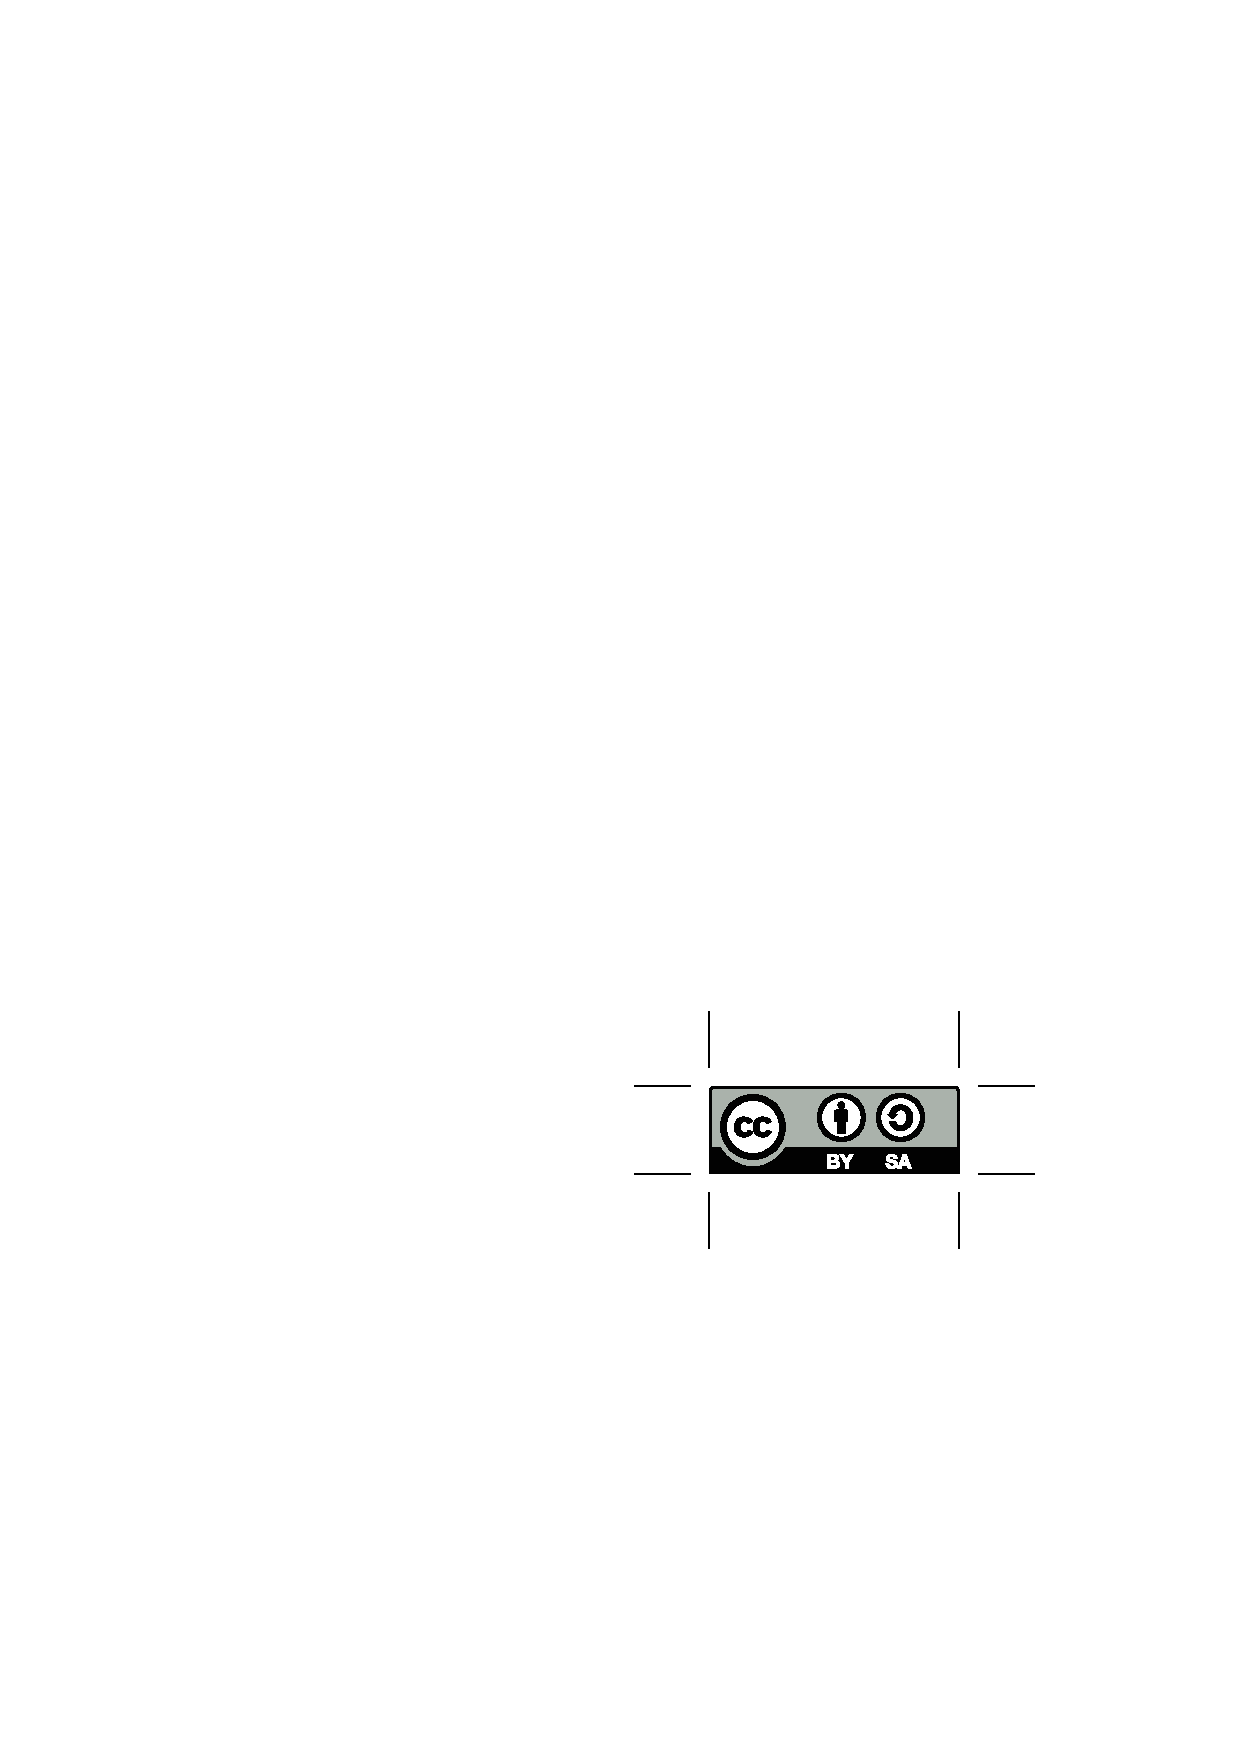
\includegraphics[width=.15\textwidth]{by-sa}
\doublespacing
% }}}

\chapter{Acknowledgements} %{{{

%}}}

% Contents {{{
\cleardoublepage
\addcontentsline{toc}{chapter}{\contentsname}
\tableofcontents
% %}}}

% List of figures {{{
\cleardoublepage
\addcontentsline{toc}{chapter}{\listfigurename}
\listoffigures
%}}}

% List of tables {{{
\cleardoublepage
\addcontentsline{toc}{chapter}{\listtablename}
\listoftables
% }}}

\mainmatter

\chapter{Introduction} % {{{

\section{Certified systems at scale} %{{{
\label{ssec:certsys}

% preamble {{{

Certified software~\citep{shao10}
is software accompanied by
a mechanized, machine-checkable proof of correctness.
To construct a certified program,
we must not only write its code in a given programming language,
but also formally specify its intended behavior
and construct, using specialized tools,
evidence that the program
indeed conforms to the specification.

%To achieve this,
%we need formal models of
%the languages in which
%the programs and other systems we wish to certify
%are described.
%The tools used to reason about them
%should be sound with respect to these models.
%Ideally,
%this will be demonstrated in an established,
%general-purpose proof assistant,
%diminishing the possibility that
%incorrect programs will be validated because of
%accidental or deliberate mistake
%in the software used to construct and check proofs.

The past decade has seen an explosion
in the scope and scale of practical software verification.
Researchers have been able to produce certified
compilers \citep{compcert},
program logics \citep{vst},
operating system kernels \citep{sel4,popl15},
file systems \citep{fscq},
processor designs \citep{safe,kami} and more,
often introducing new techniques
and mathematical models.
In this context,
there has been increasing interest in
making these components
interoperable and
combining them---and their proofs of correctness---%
into larger certified systems.

%}}}

\subsection{The DeepSpec project} %{{{

For example, the DeepSpec project \citep{deepspec}
seeks to connect various components
specified and verified in the Coq proof assistant.
The key idea behind DeepSpec
is to use specifications as \emph{interfaces}
between components.
When a component providing a certain interface
has been verified,
client components can rely on this
for their own proofs of correctness.
Standardizing this process would make it possible
to construct large-scale certified systems
by assembling off-the-shelf certified components.

This approach promises benefits
beyond the potential increase in the scale of
certified systems.
As it stands,
a certified system is only
as trustworthy as its specification.
Indeed,
it is possible to prove a buggy system correct
with respect to a buggy specification.
If the only user of the specification
is a human expert subjecting it to careful examination,
these bugs could go unnoticed
and persist in the final system.
By contrast,
if the same specification is used as a premise
in the correctness proof of a client component,
its deficiencies will become apparent
and prevent us from carrying out this second proof.

Moreover,
internal specifications used
as intermediate steps
in the verification of a complex system
disappear from the external characterization of the system,
and no longer need to be trusted.
This reduces the ratio between the size of the system
and the size of the specification
which must be trusted and understood
to establish guarantees about the overall system.

%}}}

\subsection{CompCert} %{{{

To an extent,
these principles are already demonstrated in the structure of the
certified C compiler CompCert \citep{compcert}.
In addition to the code of the compiler itself,
CompCert comes with a proof of correctness
showing that if the compiler successfully transforms
a source program $p$ into a target program $p'$,
then the behavior of $p'$ refines that of $p$:
\[
  \begin{prooftree}
    \hypo{\kw{CompCert}(p) = p'}
    \infer1{\kw{Clight}[p] \supseteq \kw{Asm}[p']}
  \end{prooftree}
\]
In the statement above,
the semantics of the source and target programs
are expressed as the sets of traces
$\kw{Clight}[p]$ and $\kw{Asm}[p']$.
Each trace record a possible execution of the corresponding program
as a sequence of events.
The trace containment property
$\kw{Clight}[p] \supseteq \kw{Asm}[p']$
expresses that any possible behavior of
the target program~$p'$
is a possible behavior of the source program~$p$.
Like the other components encompassed by the DeepSpec project,
CompCert was specified and verified
in the Coq proof assistant.

The key to this achievement
was the decomposition of CompCert
into compilation passes,
which were then specified and verified individually.
When passes are composed to obtain the overall
C-to-assembly compiler
(Fig.~\ref{fig:compcert}),
their correctness proofs can be composed as well
to construct a proof for the whole compiler.
The final theorem does not mention the intermediate
programs or language semantics,
so that a user only needs to trust
the accuracy of the C and assembly semantics,
and the soundness of the proof assistant.

\begin{figure}
  \[
    \begin{prooftree}
      \hypo{p}
      \infer1[$\kw{Clight}$]{\module{\kw{SimplLocals}} }
      \infer1[$\kw{Clight}$]{\module{\kw{Cshmgen}} }
      \infer1[$\kw{Csharpminor}$]{\rule[-1em]{0pt}{3em}\vdots}
      \infer1[$\kw{Linear}$]{\module{\kw{Linarize}} }
      \infer1[$\kw{Mach}$]{\module{\kw{Asmgen}} }
      \infer1[$\kw{Asm}$]{p'}
    \end{prooftree}
    \qquad \Rightarrow \qquad
    \begin{prooftree}
      \hypo{p}
      \infer1[$\kw{Clight}$]{\module{\rule[-5em]{0pt}{11em}\kw{CompCert}} }
      \infer1[$\kw{Asm}$]{p'}
    \end{prooftree}
  \]
  \caption[Structure of the certified compiler CompCert]%
   {Structure of the certified compiler CompCert.
    The source program $p$ is progressively transformed
    into the target program $p'$ by successive compilation passes,
    depicted here as rectangular boxes.
    The horizontal line above each compilation pass
    depicts its source language,
    and the one below depicts its target language.
    Two passes %and their semantic preservation properties
    can be composed when the target language of the first one
    corresponds to the source language of the second one.
    See also Table~\ref{tbl:passes}.}
  \label{fig:compcert}
\end{figure}

The introduction of CompCert a decade ago
represented a breakthrough
in the scale and feasability of
certified software.
Since then,
CompCert itself
has been used as a platform other projects have built upon.
For example,
verification tools have been created with soundness proofs
connecting to CompCert \citep{vst,verasco}, and
the composition techniques used to verify CompCert
have been extended in various directions
\citep{compcompcert,sepcompcert,compcertm}.

%}}}

\subsection{CertiKOS} %{{{

The techniques used in CompCert
also provided a blueprint for the verification of
the operating system kernel CertiKOS
\citep{popl15,ccal,osdi16}.
CertiKOS is divided into
several dozen \emph{certified abstraction layers},
which we specified and verified individually.

\emph{Layer interfaces} provide
an abstract view of a layer's functionality,
hiding the procedural details and low-level data representations
involved in its implementation.
They enumerate the primitives implemented by the layer
and specify their behavior.
Client code can be verified in terms of
this abstract view
in order to build higher-level layers.

To make this possible,
we extended the CompCert semantics
to be parametrized by a layer interface:
the expression $\kw{Asm}[C, L]$
denotes the set of traces generated by the client program $C$
running on top of the layer interface $L$.
Then a layer $M$
implements an \emph{overlay} interface $L_2$
on top of an \emph{underlay} interface $L_1$,
when the following \emph{contextual refinement}
property holds:
\[
  \forall \, C \, \bdot \,
    \kw{Asm}[C, L_2] \supseteq \kw{Asm}[C + M, L_1] \,.
\]
Here,
the execution of the client code $C$ on top of the overlay $L_2$
serves as the specification.
The property shows that this specification
can be implemented
by running $C$ together with the layer implementation $M$
on top of the underlay interface $L_1$.

\begin{figure}
  \[
    \begin{prooftree}
      \hypo{C}
      \infer1[$\kw{TSyscall}$]{\module{M_n}}
      \infer1[$\kw{TTrap}$]{\module{M_{n-1}} }
      \infer1[$\kw{TTrapArg}$]{\rule[-1em]{0pt}{3em}\vdots}
      \infer1[$\kw{MATOp}$]{\module{M_2}}
      \infer1[$\kw{MATIntro}$]{\module{M_1}}
      \infer1[$\kw{PreInit}$]{C + M_n + \cdots + M_1}
    \end{prooftree}
    \qquad \Rightarrow \qquad
    \begin{prooftree}
      \hypo{C}
      \infer1[$\kw{TSyscall}$]{\module{\rule[-5em]{0pt}{11em}\kw{CertiKOS}} }
      \infer1[$\kw{PreInit}$]{C + \kw{CertiKOS}}
    \end{prooftree}
  \]
  \caption[Structure of the certified OS kernel CertiKOS]%
   {Structure of the certified OS kernel CertiKOS.
    Here, boxes represent certified abstraction layers
    and horizontal lines represent layer interfaces.
    The high-level client program $C$ is transformed
    into the complete low-level program $C + \kw{CertiKOS}$
    by linking it with the successive certified abstraction layers
    of CertiKOS.
    As before, the correctness properties of layers can be composed
    to derive a correctness property for the whole system.}
  \label{fig:certikos}
\end{figure}

Certified abstraction layers
with compatible interfaces can then be chained together,
in the way passes of a compiler
can be composed when the target language of one
corresponds to the source language of another,
allowing us to derive a contextual refinement property
for the whole kernel (Fig.~\ref{fig:certikos}).
The system call interface of CertiKOS is specified
by the topmost layer interface $\kw{TSyscall}$,
and the basic facilities offered by the hardware
are formalized by bottom interface $\kw{PreInit}$.
Then, decomposing $\kw{CertiKOS} = M_n + \cdots + M_1$
into 37 certified abstraction layers,
we were able to derive the overall theorem:
\[
  \forall \, C \, \bdot \,
    \kw{Asm}[C, \kw{TSyscall}]
    \supseteq
    \kw{Asm}[C + \kw{CertiKOS}, \kw{PreInit}] \,.
\]

%}}}

\subsection{Horizontal composition} %{{{

In addition to
the \emph{vertical} composition principles presented above,
CompCert and CertiKOS provide limited forms of
\emph{horizontal} composition,
which allow individual programs and layer implementations
to be decomposed futher.

In CompCert,
this is used to model \emph{separate compilation}.
While the original correctness theorem of CompCert
only characterized the compilation of a whole program,
in practice C programs are usually made up of
several \texttt{.c} files, known as \emph{compilation units}.
These program components are compiled independently,
and the results are then linked together to build
an executable image.
To reflect this,
\citet{sepcompcert} generalized the correctness theorem of CompCert
to the separate compilation property:
\[
  \begin{prooftree}
    \hypo{\forall \, 1 \le i \le k \, \bdot \,
      \kw{CompCert}(p_i) = p_i'}
    \infer1{\kw{Clight}[p_1 + \cdots + p_k] \supseteq
      \kw{Asm}[p_1' + \cdots + p_k']}
  \end{prooftree}
\]

Likewise,
in CertiKOS the verification of a given
certified abstraction layer
can be further decomposed into
the verification of the individual functions
which constitute the layer's implementation.
This is achived through the \emph{layer calculus}
which I present in \S\ref{sec:cal}.

%}}}

\subsection{Challenges} %{{{

The compositional approach to verification presented above is compelling,
but applying it to build larger-scale certified systems
out of disparate certified components
is challenging.
A key aspect enabling composition in CompCert and CertiKOS
is the uniformity of the models underlying
their language semantics and correctness proofs.
By contrast,
across certified software projects
there exist a great diversity
of semantic models and verification techniques.
This makes it difficult to formulate
interface specifications connecting specific components,
let alone devise a general system
to express such interfaces.

Worse yet,
this diversity is not simply a historical accident.
The semantic models
used in the context of individual verification projects
are often carefully chosen
to make the verification task tractable.
The semantic model used in CompCert alone
has changed multiple times,
addressing new requirements and techniques
that were introduced alongside
new compiler features and optimizations~\citep{compsem}.
Given the difficulty of verification,
preserving this flexibility is essential.

Then,
to make it possible to link components
verified using a variety of paradigms,
we need to identify a model
expressive enough to embed
the semantics, specifications and correctness proofs
of all these paradigms.
To enable constructing large-scale certified systems,
the model should provide
high-level composition and reasoning principles.

%}}}

%}}}

\section{General models for system behaviors} %{{{
\label{ssec:genmodel}

Fortunately,
there is a wealth of semantics research to draw from
when attempting to design models for this task.

\subsection{Symmetric monoidal categories} %{{{

As a whole,
category theory provides a general study
and taxonomy for
compositional structures found
across mathematics (\S\ref{sec:cat}).
In a category,
components (morphisms) can be chained together when
the target interface (object) of one matches
the source interface of another.
For example,
compilation passes and certified abstraction layers
both constitute categories.

Symmetric monoidal categories
additionally provide a \emph{tensor product} construction,
allowing components to be connected
both in series~($\circ$) and in parallel~($\otimes$):
\[
  \begin{prooftree}
    \hypo{f : A \rightarrow B}
    \hypo{g : B \rightarrow C}
    \infer2{g \circ f : A \rightarrow C}
  \end{prooftree}
  \qquad
  \begin{prooftree}
    \hypo{f_1 : A_1 \rightarrow B_1}
    \hypo{f_2 : A_2 \rightarrow B_2}
    \infer2{f_1 \otimes f_2 : A_1 \otimes A_2 \rightarrow B_1 \otimes B_2}
  \end{prooftree}
\]
As such,
symmetric monoidal categories capture structures found
in various kinds of systems and processes \citep{rosetta}.
This basic setup can be refined by introducing additional structures,
for instance modeling
feedback loops (traced monoidal categories) or allowing
wires to run in both directions
(closed monoidal categories).

Symmetric monoidal categories appear in different forms
in many approaches to logic and programming language semantics.
For example,
\emph{cartesian closed categories}
correspond
to models of the simply typed lambda calculus,
and are a special case of symmetric monoidal categories.
However,
%in contrast with the stronger notion of
%cartesian closed category,
symmetric monoidal categories in general do not require
multiple components to be able to connect to the same interface
($\Delta : A \rightarrow A \otimes A$),
giving us more freedom to model access to shared resources.
In the same way the simply-typed lambda calculus provides
an internal language for cartesian closed categories,
various fragments of \emph{linear logic} provide
internal languages for various kinds of symmetric monoidal categories.

For our purposes,
the theory of symmetric monoidal categories
constitutes a repository of algebraic structures
formalizing the compositional aspects of
all kinds of systems,
and can be used as a blueprint
as we attempt to design general models
for certified heterogenous systems.

%}}}

\subsection{Game semantics} %{{{

A specific way to construct symmetric monoidal categories
is \emph{game semantics} \citep{cspgs},
which uses two-player games to describe
the form of the interaction between a program component and its environment,
and represents the externally observable behavior
of the component as a strategy in this game
(\S\ref{sec:bg:gamesem}).

Game semantics represents a synthesis
of various approaches to programming language semantics.
Game semantics is a form of \emph{denotational semantics},
defining the behavior of complex programs
in terms of the behavior of their components.
However,
since it models components
in terms of their interactions across time,
game semantics also provides a strong \emph{operational} flavor.
Finally,
the usual construction of strategies in game semantics
shares characteristics with the \emph{trace semantics}
used in the context of process algebra
and concurrent semantics.

An early success of this approach
was the formulation of the first
fully complete models for
the functional programming language PCF \citep{pcfajm,pcfho}.
Since then,
game semantics have provided fully complete models
for a wide variety of other languages,
incorporating features such as
state \citep{gsia},
control \citep{gscontrol},
general references \citep{gsgr},
concurrency \citep{gsconcur}
and more.
There are deep connections between
game semantics and linear logic \citep{gsnecessary},
and hence symmetric monoidal categories,
hinting to its promise
as a general approach for modeling the behavior of
various kinds of systems and processes.
In particular,
the typed aspect of many game models
makes them relevant for
describing the behavior of heterogeneous systems.

However,
the generality of game models
often translates to a fair amount of complexity,
which imposes a high barrier to entry for practitioners
and makes them difficult to formalize in a proof assistant.

%}}}

\subsection{Algebraic effects} %{{{

While more restricted,
the framework of \emph{algebraic effects} \citep{effadq}
is sufficient for many modeling tasks,
fits within the well-known monadic approach
to effectful and interactive computations,
and can be adapted into a particularly simple version
of game semantics.

In this framework,
computations are modeled as \emph{terms}
in an algebra whose operations correspond to
the available effects (\S\ref{sec:eff}).
The computation proceeds inward,
with each function symbol representing an occurence of an effect,
and each argument representing a possible way
for the computation to be continued
after the effect has been triggered.

One major advantage of this approach is that
the methods and results of universal algebra
become available to reason about effectful computations.
Equational theories can be used to characterize
the behavior of effects, and \emph{interpretations}
of one effect algebra into another can be used to model
\emph{effect handlers} \citep{eff}.
The \emph{free monad} associated to an algebra
can be used to recover the more familiar
monadic model of computational effects \citep{monads}.
Along these lines,
\emph{interaction trees} \citep{itree}
have been developed for use in and across
several DeepSpec projects.

Alegbraic effects can also be understood as
a limited form of game semantics:
signatures can be interpreted as simple games,
and the abstract syntax trees of terms
can be interpreted as strategies.
However,
their restriction to first-order computation
make them easier to formalize and reason about
than more general notions of games.

%\section{General formulations for correctness proofs}
%\label{ssec:genform}

%}}}

\subsection{The refinement calculus} %{{{

Finally,
while game models have been proposed
for a wide variety of programming languages,
there has been comparatively less focus
on specifications and correctness properties.
%in the context of game semantics.
By contrast,
the general approach of \emph{stepwise refinement}
suggests a uniform treatment of programs and specifications
as well as their relationships.
It has been studied extensively in the context of
Dijkstra's predicate transformer semantics \citep{gc}
and in the framework known as the \emph{refinement calculus} \citep{refcal}.

In refinement-based approaches,
programs and specifications are expressed in a common language,
and a certified program is constructed in an incremental manner,
by applying a series of correctness-preserving transformation
to the (abstract and declarative) specification
until we obtain a (concrete and executable) program.
Correctness preservation is expressed
by a reflexive and transitive \emph{refinement relation}.
Language constructions are monotonic with respect to this relation,
so that elementary refinement rules
can be applied congruently within any program context.

To make it possible to express specifications,
the language is extended with non-executable constructions,
including in particular infinitary versions of both
\emph{angelic} and \emph{demonic} nondeterministic choice operators.
In its modern presentation,
the refinement calculus is formulated in a lattice-theoretic framework
where joins ($\sqcup$) and meets ($\sqcap$)
correspond respectively to angelic and demonic choices.
The resulting language is remarkably expressive
and requires very few additional primitive constructions.
The duality inherent in this approach
also lends itself to game-theoretic interpretations,
and indeed the semantics of the refinement calculus
can be expressed as a two-player game between
the angel and the demon \citep[\S 14]{refcal}.

%Like all approaches in the lineage of Hoare logic
%and predicate transformer semantics,
%the refinement calculus is limited to
%modeling imperative programs.
%[However,
%M\&T propose to extend it to terms and functional programming
%by constructing the FCD blah blah.]
%
%[Also: describe the idea of the \emph{refinement calculus hierarchy}
%(general and difficult <-> specific and easy to reason about
%and string properties).
%More than one level of ``semantics''
%Notions of ``syntax'' and ``semantics'' are relative concepts.]

%}}}

%}}}

\section{Contributions} %{{{
\label{ssec:contrib}

The central claim if this dissertation is that a synthesis
of %the existing research on
game semantics, algebraic effects, and the refinement calculus
can be used to construct a hierarchy of semantic models
suitable for constructing large-scale, heterogeneous certified systems.
My contributions are twofold.

\subsection{General-purpose models for certified systems} %{{{

To provide evidence for this claim,
I outline general techniques
which can realize this synthesis
and demonstrate their use
in the context of certified abstraction layers:
\begin{itemize}
\item
  I describe in \S\ref{sec:cal}
  the theory of certified abstraction layers
  used in the verification of CertiKOS.
  The version I present is decoupled from
  CompCert semantics,
  yielding a simpler model
  which nontheless captures
  the essential features of the original.
\item
  In \S\ref{sec:games-dnd},
  I adapt the work of Morris and Tyrrell \citep{augtyp,dndf},
  which extends the refinement calculus to the level of terms
  using \emph{free completely distributive completions} of posets,
  to investigate \emph{dual nondeterminism}
  in the context of game semantics
  %Using the free completely distributive completion
  %instead of downsets when constructing strategies
  %yields
  and construct
  completely distributive lattices of
  \emph{strategy specifications},
  partially ordered
  under a form of alternating refinement
  \citep{altref}.
\item
  In \S\ref{sec:intspec},
  I define a version of the
  \emph{free monad on an effect signature}
  which incorporates dual nondeterminism and refinement.
  The result can be used to formulate a theory of certified abstraction
  layers in which
  layer interfaces, layer implementations, and simulation relations
  are treated uniformly and compositionally.
\item
  In \S\ref{sec:gamesem},
  I outline a more general category of games and
  strategy specifications;
  its object are effect signatures regarded as games
  and its morphisms specify well-bracketed strategies.
  The behavior of certified abstraction layers
  can then be represented canonically,
  and reentrant layer interfaces can be modeled.
\end{itemize}

The model presented in \S\ref{sec:intspec} was designed to be simple but
general enough to embed CompCert semantics, certified
abstraction layers, and interaction trees. The main purpose for
the model presented in \S\ref{sec:gamesem} is then to hide state and
characterize certified abstraction layers through
their externally observable interactions only.

Note that rather than providing
denotational semantics for specific programming
languages, our models are intended as a coarse-grained composition
``glue'' between components developed and verified in their own
languages, each equipped with their own internal semantics.
In this context,
the models' restriction to first-order computation
applies only to cross-component interactions,
but individual components can still make use of
high-order languages and reasoning techniques
\citep{hosl-fo}.

%and conforms to our interest in connecting
%low-level system components.

%They could be embedded in turn
%into more general game models, for instance where concurrency
%could be expressed in a more natural way.

%}}}

\subsection{CompCertO} %{{{

Given the importance of compilers in
the construction of present-day computer systems,
and of CompCert in the formal methods landscape,
its integration to any framework
attempting to tackle end-to-end verification
should be a litmus test.
%For the framework to be general,
%it cannot be designed around CompCert itself.
However, this new application of CompCert also
comes with its own challenges.

The second part of this thesis presents CompCertO,
the first extension of CompCert suitable for
these purposes:
\begin{itemize}
\item
  In \S\ref{sec:compcert-sem},
  I summarize the approach to semantics and correctness
  used in CompCert,
  as well as extensions
  which have been proposed
  to make the correctness theorem of CompCert
  more compositional.
  Game semantics and dual nondeterminism
  provide a powerful lens
  through which the existing design and extensions
  can be examined and understood.
  Going beyond the idea of a
  \emph{certified compiler},
  I then identify a set of requirements
  for using CompCert as a
  \emph{compiler of certified components}.
\item
  The design of CompCertO is presented in \S\ref{sec:compcerto}.
  CompCertO is the first extension of CompCert which
  satisfies all of the requrements I have identified.
  It generalizes the semantic model
  to express interactions between compilation units,
  using \emph{language interfaces}
  to describe the form of these interactions
  and \emph{simulation conventions}
  to describe the correspondence between the interfaces
  of source and target languages.
  The behavior of
  composite programs is specified by a
  \emph{horizontal composition} operator
  which is shown to be correctly implemented
  by the existing linking operator for assembly programs.
  To combine and reason about simulation proofs,
  we introduce a rich \emph{simulation convention algebra}
  and use it to derive our main compiler correctness statement.
\item
  Compositional relational reasoning within CompCertO
  is explained in \S\ref{sec:cklr}:
  \emph{CompCert Kripke logical relations}
  unify CompCert's memory transformations
  as structure-preserving relations
  over the memory model.
  They can be used to define simulation conventions
  for most of the compiler's passes,
  and to derive parametricity theorems which capture
  important properties of CompCert languages.
\item
  Several passes of CompCert use
  typing and soundness invariants.
  \S\ref{sec:inv} explains how these invariants fit
  into the simulation framework of CompCertO and
  how the techniques used to verify these passes
  can be reified into a notion of
  \emph{simulation modulo invariants}.
\item
  Finally, \S\ref{sec:backend}
  discusses the more specialized simulation conventions
  used for the passes of CompCert which significantly transform
  the shape of interactions across compilation units.
\end{itemize}

The simulation proofs for
most of CompCert's passes
can be updated with minimal effort.
%In the case of more complex passes,
Simulation conventions can be defined
which capture the internal invariants
used by existing proofs,
avoiding many sources of complexity found
in previous work.

%We discuss related work in \S\ref{sec:rw}
%and %conclude with a short evaluation of
%the significance of our results in \S\ref{sec:concl}.

%[The public URL of the CompCertO repository is omitted
%for the purposes of the double-blind review process
%but has been provided in HotCRP alongside this submission.]

%}}}

% }}}

% }}}

\part{Preliminaries}

\chapter{Background} % {{{

\section{Building certified systems} \label{sec:principles} %{{{

\subsection{Semantic domains} %{{{

The goal of certified system design is
to create a formal description of
the system to be constructed (the program),
while ensuring
through careful analysis
that the system
will behave properly.
To this end,
we assign
to every system $p \in P$
a mathematical object $\llbracket p \rrbracket \in \mathbb{D}$
representing its behavior.
We will call the set $\mathbb{D}$ a \emph{semantic domain}.

\begin{example}[Trace semantics]
In the original CompCert semantics,
discussed in detail in \S\ref{sec:compcert-sem},
the behaviors of programs are ultimately expressed
as sets of \emph{traces}.
Each trace records a possible execution of the program
as a finite or infinite sequence of externally observable events
taken from a set $\mathbb{E}$.
In this case, the semantic domain can be defined as
$
  \mathbb{D}_\kw{CompCert} :=
    \mathcal{P}(\mathbb{E}^* + \mathbb{E}^\omega)
$.
\end{example}

In the remainder of this section we elucidate
the structure and properties of $\mathbb{D}$
necessary to the process of building
large-scale certified systems.

%}}}

\subsection{Specifications and refinement} %{{{

System design starts with a set of requirements
on the behavior of the system to be constructed
(the specification).
These requirements do not capture every detail
of the eventual system,
but delineate a range of acceptable behaviors.

In refinement-based approaches,
programs and specifications are interpreted in the same
semantic domain $\mathbb{D}$,
which is equipped with a \emph{refinement} preorder
${\refby} \subseteq \mathbb{D} \times \mathbb{D}$.
The proposition $\sigma_1 \refby \sigma_2$
asserts that $\sigma_1$ is refined by $\sigma_2$.
The correctness of a system description $p \in P$
with respect to a specification $\sigma \in \mathbb{D}$
can then be formulated as
$\sigma \refby \llbracket p \rrbracket$.

Refinement is a correctness-preserving relation,
in the sense that for a set
$\mathbb{P} \subseteq \mathcal{P}(\mathbb{D})$
of properties of interest
and two semantic objects $\sigma_1, \sigma_2 \in \mathbb{D}$:
\[
  \sigma_1 \refby \sigma_2 \:\Rightarrow\:
  \forall P \in \mathbb{P} \bdot
    P(\sigma_1) \Rightarrow P(\sigma_2) \,.
\]

\begin{example}[Trace containment]
In the trace semantics of CompCert,
the set of traces associated with the source program
is understood as a set of \emph{permissible} behaviors
for the target program.
The corresponding notion of refinement is
\emph{trace containment},
expressed by the superset relation $\supseteq$.
For instance
$\kw{Clight}[p] \in \mathbb{D}_\kw{CompCert}$
is refined by
$\kw{Asm}[p'] \in \mathbb{D}_\kw{CompCert}$
when
$
  \kw{Clight}[p] \supseteq \kw{Asm}[p']
$.

Any property $P(\sigma)$
asserting that \emph{all} traces
$t \in \sigma$
satisfy a given condition
will be preserved by trace containment.
\end{example}

%}}}

\subsection{Compositionality} %{{{

Complex systems are built by assembling components
whose behavior is understood,
such that their interaction achieves a desired effect.
The syntactic constructions of
the language used to describe systems
correspond to the ways in which they can be composed.

To enable compositional reasoning,
a suitable model must provide an account of
the behavior of the composite system
in terms of the behavior of its parts.
For instance,
if the language contains a binary operator
${+} : P \times P \rightarrow P$,
then the semantic domain should be equipped with
a corresponding operation
${\oplus} : \mathbb{D} \times \mathbb{D} \rightarrow \mathbb{D}$.
Ideally,
the operation $\oplus$
will characterize $+$ exactly:
\begin{equation}
  \llbracket p_1 \rrbracket \oplus \llbracket p_2 \rrbracket
  =
  \llbracket p_1 + p_2 \rrbracket
  \,.
  \label{eqn:compositionality}
\end{equation}

\begin{example}
Denotational semantics are compositional by nature.
The behavior of program components
is defined recursively on their structure,
so that (\ref{eqn:compositionality}) holds \emph{by definition}.
\end{example}

In the context of refinement-based verification,
we can regard $\oplus$ as a \emph{specification} for $+$,
and it is sufficient to establish that:
\begin{equation}
  \llbracket p_1 \rrbracket \oplus \llbracket p_2 \rrbracket
  \refby
  \llbracket p_1 + p_2 \rrbracket \,.
  \label{eqn:compositional-correctness}
\end{equation}

\begin{example}[Linking in CompCertO]
In the semantic model of CompCertO (\S\ref{sec:compcerto}),
the horizontal composition operation $\oplus$ on component semantics
provides a specification for
CompCert's program linking operation $+$.
This operation acts as a specification for linking.
In particular, the correctness of assembly linking
is established in Thm.~\ref{thm:asmlinking} as
$
  \kw{Asm}(p_1) \oplus \kw{Asm}(p_2) \refby
  \kw{Asm}(p_1 + p_2)
$.
\end{example}

%}}}

\subsection{Monotonicity} %{{{

Once a component has been shown to conform to a given specification,
we want to abstract it as a ``black box''
so that further reasoning can be done in terms of
the component's specification rather than its implementation details.
To support this,
we must establish that semantic composition operators
are compatible with refinement:
\[ \sigma_1 \refby \sigma_1' \wedge
   \sigma_2 \refby \sigma_2' \Rightarrow
   \sigma_1 \oplus \sigma_2 \refby \sigma_1' \oplus \sigma_2' \,. \]
Suppose we have two components $p_1$ and $p_2$,
where $p_2$ relies on $p_1$ for its operation,
and we want to verify that their combination $p_1 + p_2$
satisfies a specification $\sigma$.
Once we verify $p_1$ against its own specification
$\sigma_1 \refby \llbracket p_1 \rrbracket$,
by the monotonicity of ${\oplus}$ it is sufficient to show that
$\sigma \refby \sigma_1 \oplus \llbracket p_2 \rrbracket$:
\[
   \sigma \:\refby\:
   \sigma_1 \oplus \llbracket p_2 \rrbracket \:\refby\:
   \llbracket p_1 \rrbracket \oplus \llbracket p_2 \rrbracket \:\refby\:
   \llbracket p_1 + p_2 \rrbracket \,.
\]

%}}}

\subsection{Types} %{{{

In most cases,
systems are built out of components of various types
which can only be composed when their types are compatible.
Different semantic domains can then be used
to interpret components of different types.

Categories provide a principled algebraic framework
to realize this separation.
Instead of a single set $\mathbb{D}$,
we use a category $\mathbf{D}$.
The objects $A \in \mathbf{D}$ correspond to
the possible types or interfaces alongside which
components can be connected.
The behavior of components which
use an interface $A$ to
implement an interface $B$
can then be interpreted as morphisms
of type $A \rightarrow B$.
Category theory can then be a useful resource
to formulate and characterize typed composition principles,
and the theory of \emph{enriched categories}
can be used to explore how these composition principles
interact with the structure of the semantic domains
$\mathbf{D}(A, B)$.

%\begin{example}[Denotational semantics of type theories]
%Categorical semantics of type theories
%usually interpret types and typing contexts as objects,
%and terms and substitutions as morphisms.
%For instance,
%consider a calculus with a base type $\mathbb{N}$
%and a built-in addition operation
%associated with the typing rule:
%\[
%  x : \mathbb{N}, y : \mathbb{N} \vdash x + y : \mathbb{N} \,.
%\]
%To give a semantics to the calculus,
%we must first choose a category $\mathbf{C}$ with finite products.
%Products are used to interpret contexts with multiple variables
%($x : \mathbb{N}, y : \mathbb{N}$)
%as well as product types when they are available
%($\mathbb{N} \times \mathbb{N}$).
%We then give an object
%$\llbracket \mathbb{N} \rrbracket \in \mathbf{D}$
%to interpret the type $\mathbb{N}$,
%and a morphism
%$\kw{plus} :
% \llbracket \mathbb{N} \rrbracket \times
% \llbracket \mathbb{N} \rrbracket \rightarrow
% \llbracket \mathbb{N} \rrbracket$
%to interpret the $+$ operation.
%\end{example}

\begin{example}[Signatures]
The models introduced in this thesis use \emph{signatures}
to enumerate the operations used and provided by program components.
Consequently,
the semantics of components are expressed in categories
whose objects are signatures.
Morphisms of type $E \rightarrow F$
describe the behavior of components 
which use the operations of $E$
to implement the operations of $F$.
Categorical structures can then be used to
describe various composition principles
(see \S\ref{sec:cal} for example).
\end{example}

%}}}

\subsection{Abstraction} %{{{

Large-scale systems operate across multiple levels of abstraction.
Each level brings to its own understanding of the interaction
between a component and its environment.
To reason across abstraction layers we need to give
an explicit account of how these different views
of a component's interactions
correspond to one another.

This is studied extensively
in the context of abstract interpretation \citep{aif}.
Suppose $\mathbb{D}_1$ is the concrete domain
and $\mathbb{D}_2$ is the abstract one.
To establish a correspondence between them,
the most general approach is to define a \emph{soundness relation}
$\rho \subseteq \mathbb{D}_2 \times \mathbb{D}_1$.
%
%\begin{example}[Calling conventions]
%Abstraction is particularly relevant
%in the context of compilers.
%For example, between C and assembly,
%interactions across compilation units
%are understood very differently.
%At the level of C,
%cross-module interaction is defined in terms of
%function calls;
%invoking a function consists of assigning values
%to the function's parameters,
%initializing a new stack frame,
%and finally executing the function's body.
%At the assembly level, cross-module
%interactions simply consist in branching to an address
%outside of the current module with
%a certain register state.
%
%In that context,
%the correpondance between the source and target semantic domains
%depends on the \emph{calling convention} used by the compiler.
%The correctness property of a C-to-assembly compiler
%can then be stated as:
%$
%  \llbracket p \rrbracket_s \mathrel{\rho}
%  \llbracket C(p) \rrbracket_t
%$,
%where
%$p$ is the source program, $C(p)$ the compiler's output,
%$\llbracket - \rrbracket_s$ gives the semantics of the source language,
%$\llbracket - \rrbracket_t$ gives the semantics of the target language,
%and the soundness relation $\rho$ formalizes the C calling convention.
%\end{example}

Often there will be a more elementary description
of the correspondence,
based on the construction of the semantic domains,
as illustrated by the following example.

\begin{example}
In the model of \emph{certified abstraction layers}
presented in \S\ref{sec:cal},
the semantic domain used to represent layer interfaces,
is parametrized by a set of abstract states $S$.
To compare a layer interface formulated in terms of
a more concrete set of states $S_1$ with
a layer interface formulated in terms of
a more abstract set of states $S_2$,
we will use a relation $R \subseteq S_2 \times S_1$.
This relation can then be extended to the level of layer interfaces
as a soundness relation
${\le_R} \subseteq \mathbb{D}[S_2] \times \mathbb{D}[S_1]$,
asserting that $R$ is a simulation relation between
a layer interface in $\mathbb{D}[S_2]$ and
a layer interface in $\mathbb{D}[S_1]$.
\end{example}

In any case,
we expect $\rho$
to be compatible with refinement:
\[
  \begin{prooftree}
    \hypo{\sigma_2' \refby_2 \sigma_2}
    \hypo{\sigma_2 \mathrel{\rho} \sigma_1}
    \hypo{\sigma_1 \refby_1 \sigma_1'}
    \infer3{\sigma_2' \mathrel{\rho} \sigma_1'}
  \end{prooftree}
\]
In other words,
if $\sigma_2$ is an abstraction which soundly approximates
a concrete semantic object $\sigma_1$,
making $\sigma_2$ less precise or $\sigma_1$ more precise
preserves this relationship.

In the case of categorical semantics
where $\mathbb{D}_1 = \mathbf{D}(A_1, B_1)$
and $\mathbb{D}_2 = \mathbf{D}(A_2, B_2)$
are homsets,
the constituents of the soundness relation
may themselves be organized as a category
with the same objects as $\mathbf{D}$.
This induces a double category structure,
where horizontal morphisms are the semantic objects,
vertical morphisms are abstraction relationships,
and 2-cells correspond to the soundness relation.

When the semantic domains are rich enough,
there will be a most precise $\sigma_2$
corresponding to each $\sigma_1$,
and a least precise $\sigma_1$
corresponding to each $\sigma_2$,
allowing us to define
a concretization function
$\gamma : \mathbb{D}_2 \rightarrow \mathbb{D}_1$
and an abstraction function
$\alpha : \mathbb{D}_1 \rightarrow \mathbb{D}_2$
such that:
\[
  \gamma(\sigma_2) \refby_1 \sigma_1
  \quad \Leftrightarrow \quad
  \sigma_2 \mathrel{\rho} \sigma_1
  \quad \Leftrightarrow \quad
  \sigma_2 \refby_2 \alpha(\sigma_1) \,,
\]
This corresponds to
the original formulation of abstract interpretation \citep{absint}
in terms of Galois connections \citep{pgc}.

\begin{example}[Simulation conventions in CompCertO]
In the model used in CompCertO (\S\ref{sec:compcerto}),
\emph{language interfaces} play the role of objects,
and semantic domains assigned a type $A \rightarrow B$
where $A$ and $B$ are language interfaces.
In addition,
a \emph{simulation convention}
$\mathbb{R} : A \Leftrightarrow B$
is used to formulate the correspondence between
the high-level language interface $A$ and
the low-level language interface $B$.
A typical simulation property can be depicted as the 2-cell:
\[
  \begin{tikzpicture}[baseline,scale=0.66]
    \node (A1) at (-1,  2) {$A_1$};
    \node (A2) at (-1,  0) {$A_2$};
    \node (B1) at ( 1,  2) {$B_1$};
    \node (B2) at ( 1,  0) {$B_2$};
    \draw (A1) edge[->] node[auto] {$L_1$} (B1);
    \draw (A2) edge[->] node[below] {$L_2$} (B2);
    \begin{scope}[double equal sign distance, {Implies[]}-{Implies[]}]
      \draw (A1) edge[double] node[auto,swap] {$\mathbb{R}_A$} (A2);
      \draw (B1) edge[double] node[auto] {$\mathbb{R}_B$} (B2);
    \end{scope}
  \end{tikzpicture}
\]
\end{example}

%}}}

\subsection{Embedding} %{{{

It is often useful to first interpret the semantics of a component
in a more restricted domain,
then embed this domain into a more general one:
\[
    p \in P \xrightarrow{\llbracket - \rrbracket}
    \sigma \in \mathbb{D} \xrightarrow{|-|}
    |\sigma| \in \mathbb{D}'
\]
The elements of the restricted domain $\mathbb{D}$
will often have stronger properties,
or be expressed in a way which makes certain
proof methods more tractable.
The more general domain $\mathbb{D}'$
can then provide more expressivity
and additional algebraic structures,
and may embed the behaviors of different kinds of components,
but may be less amenable to domain-specific reasoning.

In this situation,
we will want the embedding
$|-| : \mathbb{D} \rightarrow \mathbb{D}'$
to preserve any relevant structure present in both
$\mathbb{D}$ and $\mathbb{D}'$.
For example,
in the case of categorical semantics,
this embedding will be a functor
of the appropriate kind.

\begin{example}[Transition systems and trace semantics in CompCert] %{{{
As previously mentioned,
CompCert semantics
ultimately characterize the behavior of programs
in terms of traces.
However,
they are first defined as labelled transition systems,
and the correctness properties of compilation passes
are first proved as simulations.
An embedding then assigns to each transition system $L$
the set of traces $|L|$ characterizing
its observable behavior,
and a soundness proof shows that
simulation properties $L_1 \le L_2$
imply trace containment $|L_1| \supseteq |L_2|$.
See \S\ref{sec:compcert-sem}.
\end{example}
%}}}

\begin{example}[Certified abstraction layers] %{{{
The theory of certified abstraction layers
developped in \S\ref{sec:cal}
only describes deterministic layer interfaces
and implementations.
In this theory,
the simulation relations used to formulate abstraction
are formalized as a distinct kind of object.
In \S\ref{sec:intspec},
I show how the theory of \S\ref{sec:cal}
can be embedded into a more general framework
which supports dual nondeterminism,
allowing simulation relations
to be internalized as regular morphisms,
but making the notion of refinement more sophisticated.
Finally in \S\ref{sec:gamesem},
I outline a framework where the layers' states
can be encapsulated and hidden from
the descriptions of the layers' behaviors.
This means simulation relations are no longer necessary at all,
but prevents us from expressing the cartesian products of \S\ref{sec:cal}.
However,
each of these embeddings preserves categorical composition,
refinement, and tensor products.
\end{example}
%}}}

%}}}

%}}}

\section{The refinement calculus} % {{{

% Preamble {{{

Correctness properties for imperative programs
are often stated as triples of the form $\htr{P}{C}{Q}$
asserting that
when the program $C$ is started in a state which
satisfies the predicate $P$ (the \emph{precondition}),
then the state in which $C$ terminates
will satisfy the predicate $Q$ (the \emph{postcondition}).
For example:
\[
    \htr{\text{$\kw{x}$ is odd}\,}{\kw{x := x * 2}}{\,\text{$\kw{x}$ is even}}
\]
In the \emph{axiomatic} approach~\citep{hoare69} to programming language semantics,
inference rules
corresponding to the different constructions of the language
determine which triples are valid,
and the meaning of a program is identified with
the set of properties $\htr{P}{-}{Q}$
which the program satisfies.

\subsection{Dual nondeterminism}

Axiomatic semantics
can accommodate nondeterminism in two different ways.
In the program $C_1 \sqcap C_2$,
a \emph{demon} will choose which of $C_1$ or $C_2$ is executed.
The program $\kw{x := 2 * x} \: \sqcap \: \kw{x := 0}$
may be executed arbitrarily as $\kw{x := 2 * x}$ or $\kw{x := 0}$,
with no guarantee as to which branch will be chosen.
The demon works against us,
so that if we want $C_1 \sqcap C_2$ to satisfy a given property,
we need to make sure we can deal with either choice.
This corresponds to the inference rule:
\[
  \begin{prooftree}
    \hypo{\htr{P}{C_1}{Q}}
    \hypo{\htr{P}{C_2}{Q}}
    \infer2{\htr{P}{C_1 \sqcap C_2}{Q}}
  \end{prooftree}
\]
Conversely,
in the program $C_1 \sqcup C_2$,
an \emph{angel} will decide whether $C_1$ or $C_2$ is executed.
If possible,
the angel will make choices which validate
the correctness property.
This implies:
\[
  \begin{prooftree}
    \hypo{\htr{P}{C_1}{Q}}
    \infer1{\htr{P}{C_1 \sqcup C_2}{Q}}
  \end{prooftree}
  \qquad
  \begin{prooftree}
    \hypo{\htr{P}{C_2}{Q}}
    \infer1{\htr{P}{C_1 \sqcup C_2}{Q}}
  \end{prooftree}
\]
The statement $\kw{x := x * 2} \: \sqcup \: \kw{x := 0}$
is more difficult to interpret than its demonic counterpart,
but can be thought of as a program which magically behaves as
$\kw{x := x * 2}$ or $\kw{x := 0}$
depending on the needs of its user.

More generally,
a triple $\htr{P}{C}{Q}$
can be interpreted as a \emph{game}
between the angel and the demon \citep{refcal}.
The angel resolves the $\sqcup$ choices,
whereas the demon resolves $\sqcap$.
The triple is valid if there is a winning strategy
for the angel.

%}}}

\subsection{Distributivity} %{{{

Note that in this setup,
$\sqcap$ and $\sqcup$ distribute over each other.
More precisely, for all $P, C_1, C_2, C_3, Q$:
\begin{align*}
  \htr{P}{C_1 \sqcap (C_2 \sqcup C_3)}{Q} &\Leftrightarrow
    \htr{P}{(C_1 \sqcap C_2) \sqcup (C_1 \sqcap C_3)}{Q} \\
  \htr{P}{C_1 \sqcup (C_2 \sqcap C_3)}{Q} &\Leftrightarrow
    \htr{P}{(C_1 \sqcup C_2) \sqcap (C_1 \sqcup C_3)}{Q}
\end{align*}
Consider the first equivalence above.
If the angel has a winning strategy for
the left-hand side triple,
they can win both $\htr{P}{C_1}{Q}$
and either $\htr{P}{C_2}{Q}$ or $\htr{P}{C_3}{Q}$.
Although the right-hand side triple
reverses the angel and demon's choices,
the angel can preemptively choose the left or right
disjunct depending on whether they can win
$\htr{P}{C_2}{Q}$ or $\htr{P}{C_3}{Q}$.
Likewise, if the angel can win the right-hand side,
then they have a winning strategy for the left-hand side as well.
The second equivalence corresponds to a similar situation
where the angel and demon have been exchanged.

%}}}

\subsection{Program refinement} %{{{

Instead of proving program correctness in one go,
\emph{stepwise refinement} techniques use a more incremental approach
centered on the notion of program refinement.
A refinement $C_1 \sqsubseteq C_2$
means that any correctness property satisfied by $C_1$
will also be satisfied by $C_2$:
\[
    C_1 \sqsubseteq C_2 \: := \:
    \forall P Q \bdot
      \htr{P}{C_1}{Q} \Rightarrow
      \htr{P}{C_2}{Q}
\]
We say that $C_2$ refines $C_1$
or that $C_1$ is refined by $C_2$.

Typically,
under such approaches,
the language will be extended with constructions
allowing the user to describe
abstract specifications as well as
concrete programs.
Then the goal is to establish
a sequence of refinements
$C_1 \sqsubseteq \cdots \sqsubseteq C_n$
to show that a program $C_n$ involving
only executable constructions
correctly implements a specification $C_1$,
which may be stated in much more abstract terms.

If the language is sufficiently expressive,
then a correctness property $\htr{P}{-}{Q}$
can itself be encoded \citep{specstm} as
a specification statement $\langle{}P,Q{}\rangle$
such that:
\[
    \htr{P}{C}{Q} \: \Leftrightarrow \:
    \langle{}P,Q{}\rangle \sqsubseteq C \,.
\]
In the context of refinement,
the properties associated with demonic and angelic choice
generalize as:
\begin{align*}
  C \sqsubseteq C_1 \:\wedge\: C \sqsubseteq C_2 &
    \:\Rightarrow\: C \sqsubseteq C_1 \sqcap C_2 \\
  C \sqsubseteq C_1 \:\vee\: C \sqsubseteq C_2 &
    \:\Rightarrow\: C \sqsubseteq C_1 \sqcup C_2
\end{align*}
Given the symmetry between the demon and angel,
it is then natural to interpret demonic and angelic choices
respectively as meets and joins
of the refinement ordering.

\subsection{Nondeterministic choice in specifications}

Until this point,
we have discussed demonic ($\sqcap$) and angelic ($\sqcup$) choices
as implementation constructs
(appearing to the right of $\sqsubseteq$),
taking the point of view of a client
seeking to use the program to achieve a certain goal.
However,
in this work they are used primarily
as \emph{specification} constructs
(appearing to the left of $\sqsubseteq$),
and we are interested in what it means
for a system to implement them.
%
As a specification, $C_1 \sqcap C_2$
allows the system to refine either one of $C_1$ or $C_2$, while
$C_1 \sqcup C_2$ requires it to refine
\emph{both} of them:
\begin{gather*}
  C_1 \sqsubseteq C \: \vee \: C_2 \sqsubseteq C
    \: \Rightarrow \: C_1 \sqcap C_2 \sqsubseteq C \\
  C_1 \sqsubseteq C \: \wedge \: C_2 \sqsubseteq C
    \: \Rightarrow \: C_1 \sqcup C_2 \sqsubseteq C 
\end{gather*}
In other words,
demonic choices
give us more
implementation freedom,
whereas angelic choices make a specification
stronger and more difficult to implement.
%Intuitively,
%the \emph{user} of a specification
%will need to be ready to handle any demonic choice
%made in that specification.
%The specification's implementer
%will have more freedom because they \emph{are} the demon.
%Conversely,
%angelic choice requires the implementation
%to behave appropriately
%no matter which alternative the user decides to rely on.
%Therefore,
Therefore we can think of demonic choices as
choices of the \emph{system}, % we are considering,
and think of angelic choices as
choices of the \emph{environment}.

%}}}

\subsection{The refinement calculus} %{{{

%\jk{cut candidate}
These basic ingredients have been studied systematically
in the \emph{refinement calculus},
dating back to Ralph-Johan Back's 1978 PhD thesis \citep{backthesis}.
In its modern incarnation \citep{refcal},
the refinement calculus
subsumes programs and specifications with \emph{contracts}
featuring unbounded angelic and demonic choices.
These choice operators
constitute a completely distributive lattice
with respect to the refinement order.

Dijkstra's \emph{predicate transformer} semantics \citep{gc}
are a natural fit for the refinement calculus,
but other approaches are possible.
For instance,
the understanding of contracts as a game between
the angel and the demon
can be formalized to provide a form of
game semantics for the refinement calculus.

More generally,
The refinement calculus can be presented as a \emph{hierarchy}
where simpler models (state transformer functions, relations)
can be embedded in more general ones (predicate transformers)
in various structure-preserving ways.
This makes it possible to reason about simpler components
in a limited, stronger version of the framework,
while retaining the possibility of embedding them
in a setting
where more general constructions are available,
and where they can be composed with components
developed and analyzed in a different setting.
This expressivity is highly desirable
as a scalable approach to
verifying heterogeneous systems.

%\jk{Is this defensible?}
However,
%like all methods in the lineage of Hoare logic
the refinement calculus only applies to imperative programs
with no side-effects beyond changes to the program state.
Recent research has attempted to extend the paradigm
to a broader setting,
and the present work can be understood
as a step in this direction as well.

%}}}

%}}}

\section{Game semantics} \label{sec:bg:gamesem} %{{{

% preamble {{{

Game semantics~\citep{gsll,gamesem99}
is a form of denotational semantics which
incorporates some operational aspects.
An early success of this approach was
the formulation of the first fully abstract models
of the programming language PCF \citep{pcfajm,pcfho}.
Typically,
game semantics interpret
types as two-player games
and terms as strategies for these games.
Games describe the form of the interaction
between a program component %of the corresponding type
(the \emph{system})
and its execution context
(the \emph{environment}).
Strategies
specify which move the system plays
for all relevant positions in the game.

Positions are usually identified with sequences of moves,
and strategies with the set of positions
a component can reach.
% depending on the possible behaviors of the environment
This representation makes
game semantics similar to
trace semantics of process algebras,
but it is distinguished
by a strong polarization between
actions of the system and the environment,
and between outputs and inputs.
This confers an inherent ``rely-guarantee'' flavor
to games which facilitates compositional reasoning
\citep{cspgs}.

For example,
in a simple game semantics resembling that of
Idealized Algol \citep{gsia},
sequences of moves corresponding to
the execution of $\kw{x := 2 * x}$
have the form:
\[
    \kw{run} \cdot
    \underline{\kw{rd}_\kw{x}} \cdot n \cdot
    \underline{\kw{wr}_\kw{x}[2n]} \cdot \kw{ok} \cdot
    \underline{\kw{done}} \quad (n \in \mathbb{N})
\]
The moves of the system have been underlined.
The environment initiates the execution with
the move $\kw{run}$.
The system move $\kw{rd}_\kw{x}$ requests
the value of the variable $\kw{x}$,
communicated in response by the environment move $n$.
The system move $\kw{wr}_\kw{x}[2n]$ requests
storing the value $2n$ into the variable~$\kw{x}$,
and is acknowledged by the environment move $\kw{ok}$.
Finally, the system move $\kw{done}$
expresses termination.

%}}}

\subsection{Games} \label{sec:mainideas:gs:games} %{{{

A game is defined by a set of moves
players will choose from,
as well as a stipulation of which
sequences of moves are valid.
We focus on two-player, alternating games
where the environment plays first and
where the players
each contribute every other move.

When typesetting examples,
we underline the moves of the system.
For chess,
moves are taken in the set $\{a1 \ldots h8\} \times \{a1 \ldots h8\}$,
and a valid sequence of moves may look like:
\[ e2e4 \cdot \underline{c7c5} \cdot c2c3 \cdot \underline{d7d5} \cdots \]
The games we use to model low-level components
will rely on the following constructions.

Most game semantics
include additional structure
in the description of games.
The set of moves is usually partitioned
into proponent and opponent moves ($M = M^\kw{O} \uplus M^\kw{P}$),
and into questions and answers ($M = M^\que \uplus M^\ans$).
Game models for high-order languages are often more complex,
and include \emph{justification pointers}
encoding the causal structure of the interaction.

%While the game $\mathcal{C}$
%is extremely simple,
The expressive power of game semantics
comes from the ways in which complex games can be derived from simple ones,
and used to interpret compound types.
For example,
in the game $A \times B$
the environment initially chooses whether to play
an instance of $A$ or an instance of $B$.
The game $A \rightarrow B$ usually consists of
an instance of $B$ played
together with instances of $A$
started at the discretion of the system,
where the roles of the players are reversed.
%and which correspond to
%the multiple accesses to the argument values
%allowed by most $\lambda$-calculi.

%}}}

\subsection{Strategies} %{{{

The \emph{plays} of a game are sequences of moves;
they identify a position in the game
and describe the succession of actions that led to it.
Most game models of sequential computation
use \emph{alternating} plays,
in which
the system and environment each contribute
every other move.
It is also common to require the environment to play first
and to restrict plays to even lengths,
so that they specify which action the system took
in response to the latest environment move.
We write $P_G$ for the set of plays of the game $G$,
partially ordered by the prefix relation $\pref$.

Traditionally \citep{gamesem99},
strategies are defined as
prefix-closed sets of plays,
so that strategies $\sigma \in S_G$
for the game $G$ are downsets of $P_G$
satisfying certain requirements:
\[
    S_G \subseteq
    \mathcal{D}(P_G, {\pref})
\]
A play $s \in P_G$ can be promoted to a strategy
${\downarrow} s \in \mathcal{D}(P_G, {\pref})$:
\[
    {\downarrow} s := \{ t \in P_G \mid t \pref s \}
\]
Set inclusion corresponds to strategy refinement, %refinement of strategies,
and the downset completion augments $P_G$ with
%arbitrary
angelic choices.

%}}}

\subsection{Nondeterminism} \label{sec:bg:gsnondet} %{{{

A common constraint is that a strategy $\sigma \in S_G$
should not contain two plays $s m_1, s m_2 \in \sigma$
where $m_1$ and $m_2$ are distinct moves of the system.
This is usually understood as
enforcing \emph{system determinism}:
given a set of environment choices,
there is only one possible behavior for the system.
Therefore,
relaxing this constraint has usually been understood
as the first step toward modeling nondeterministic systems
\citep{gsfnd}.
However,
looking at the situation through the lens of
refinement and dual nondeterminism
yields to a different conclusion,
where this requirement corresponds to
\emph{environment determinacy}.

%As a poset completion,
%the downset lattice
%$\mathcal{D}(P_G, {\sqsubseteq})$
%can be understood as
%the \emph{free completely distributive join-semilattice}.
%\jk{<- drop this sentence?}

Angelic nondeterminism
allows us to range over all possible choices of the environment
and record the resulting plays.
For instance,
expressing the strategy for $\kw{x := 2 * x}$
as a prefix-closed set of even-length plays,
we get:
\begin{align*}
  \sigma := {} &
    \bigcup_{n \in \mathbb{N}} {\downarrow}(
      \kw{run} \cdot
      \underline{\kw{rd}_\kw{x}} \cdot n \cdot
      \underline{\kw{wr}_\kw{x}[2n]} \cdot \kw{ok} \cdot
      \underline{\kw{done}}) \\
        = {} & \{ \epsilon, \quad
        \kw{run} \cdot
        \underline{\kw{rd}_\kw{x}} , \quad
        \kw{run} \cdot
        \underline{\kw{rd}_\kw{x}} \cdot n \cdot
        \underline{\kw{wr}_\kw{x}[2n]} , \quad
        \kw{run} \cdot
        \underline{\kw{rd}_\kw{x}} \cdot n \cdot
        \underline{\kw{wr}_\kw{x}[2n]} \cdot \kw{ok} \cdot
        \underline{\kw{done}}
        \: \mid \: n \in \mathbb{N} \}
\end{align*}
Note that this strategy admits refinements
containing much more angelic nondeterminism,
including with respect to moves of the system.
For instance:
\[
  \sigma \subseteq
    \bigcup_{n \in \mathbb{N}} \:
    \bigcup_{-1 \le \delta \le 1}
    {\downarrow}(
      \kw{run} \cdot
      \underline{\kw{rd}_\kw{x}} \cdot n \cdot
      \underline{\kw{wr}_\kw{x}[2n + \delta]} \cdot \kw{ok} \cdot
      \underline{\kw{done}})
\]
These refinements do not correspond to interpretations
of concrete programs,
and in game models which seek to achieve definability
they are usually excluded.
In our context, retaining them is algebraically important,
and they can in fact appear as intermediate terms
in some applications.
In the construction above,
although $\delta$ appears in a system move,
it is still associated with an \emph{angelic} choice.
This can be interpreted as a choice of the environment
which is not directly observed
(perhaps as a result of abstraction),
but which nonetheless influences the behavior of the system.

%Moreover,
This is different from allowing the \emph{system}
to choose an answer in the interval $[2n - 1, 2n + 1]$.
The model and refinement lattice which
we have presented so far are insufficient
to express such a specification,
because downsets do not add enough meets,
%to weaken precisely relax the specification,
forcing the would-be specification to become
much coarser:
\[
  \sigma' :=
    \bigcup_{n \in \mathbb{N}} \:
    \bigcap_{-1 \le \delta \le 1}
    {\downarrow}(
      \kw{run} \cdot
      \underline{\kw{rd}_\kw{x}} \cdot n \cdot
      \underline{\kw{wr}_\kw{x}[2n + \delta]} \cdot \kw{ok} \cdot
      \underline{\kw{done}}) =
      \{ \epsilon,  \: \kw{run} \cdot \underline{\kw{rd}_\kw{x}} \}
    \,.
\]
We will remedy this by using a richer completion,
as explained in \S\ref{sec:games-dnd}.

%}}}

%%\subsection{Refinement} \label{sec:mainideas:gs:ref} %{{{
%
%Existing work on denotational game semantics of
%typed functional languages
%has not placed much emphasis on the notion of refinement,
%focusing instead on program equivalence and
%the problem of full abstraction.
%While there have been attempts to integrate nondeterminism
%to game semantics \citep{gsnondet,gsndsheaves},
%we believe that this work
%is limited by a lack of distinction between angelic and demonic
%nondeterminism.
%
%The distinction between system and environment actions
%present in game-theoretical approaches
%leads to a notion of \emph{alternating} refinement:
%a behavior $x$ refines a behavior $y$ if
%all \emph{system} actions in $x$ are also possible in $y$, and if
%all \emph{environment} actions in $y$ are also possible in $x$
%\citep{altref,gmos}.
%This makes it possible for specifications to
%constrain the environment as well as the system,
%and enables a rely-guarantee style of reasoning.
%
%In the realm of imperative program semantics and verification,
%it has long been recognized that predicate transformers
%can model both \emph{angelic} and \emph{demonic} nondeterminism,
%and that this duality has important connections to games.
%In particular,
%the imperative programs and specifications
%of the \emph{refinement calculus} are understood as
%\emph{contracts} between a component and its environment,
%and their behavior is described in terms of
%an operational game semantics \citep{refcal,refcalgames}.
%The calculus incorporates both kinds of nondeterminism
%as the meet and join operations of the calculus' refinement lattice.
%
%We build on recent work extending this approach to the realm
%of functional programming \citep{augtyp,dndf}
%to incorporate dual nondeterminism to the game semantics
%we present in \S\ref{sec:gamesem}.
%
%%}}}

%}}}

\section{Logical relations} % {{{

Logical relations are structure-preserving relations
in the way homomorphisms are structure-preserving maps.
However,
logical relations are more compositional than homomorphisms,
because they do not suffer from the same problems
in the presence of mixed-variance constructions
like the function arrow %$\rightarrow$
\citep{lrp}.
In the context of typed languages,
this means that type-indexed logical relations
can be defined by recursion over the structure of types.

Logical relations have found widespread use in programming language theory.
Unary logical relations can be used to establish
various properties of type systems:
a type-indexed predicate expressing a property of interest
is shown to be compatible with the language's reduction,
and to contain all of the well-typed terms of the language.
Binary logical relations can be used to capture
contextual equivalence between terms,
as well as notions such as non-interference or compiler correctness.
Relational models of type quantification yield
Reynold's well-known theory of relational parametricity,
and can be used to prove \emph{free theorems} that
all terms of a given parametric type must satisfy.

\subsection{Binary logical relations}

Logical relations can be of any arity,
but
we restrict our attention to
binary logical relations.
Given an algebraic structure $\mathcal{S}$,
a \emph{logical relation}
between two instances $S_1, S_2$ of $\mathcal{S}$
is a relation $R$
between their carrier sets,
such that the corresponding operations of $S_1$ and $S_2$
take related arguments to related results.
We write $R \in \mathcal{R}(S_1, S_2)$.

\begin{example}%[Logical relation of monoids] %{{{
\label{ex:monoid}
A monoid is a set with
an associative operation $\cdot$ and
an identity element $\epsilon$.
A~\emph{logical relation of monoids} between
$\langle A, \cdot_A, \epsilon_A \rangle$ and
$\langle B, \cdot_B, \epsilon_B \rangle$
is a relation $R \subseteq A \times B$
such that:
\begin{equation}
\label{eqn:monoidrel}
(u \mathrel{R} u' \wedge v \mathrel{R} v' \: \Rightarrow \:
 u \cdot_A v \: \mathrel{R} \: u' \cdot_B v')
\: \wedge \:
\epsilon_A \mathrel{R} \epsilon_B \,.
\end{equation}
\end{example}
%}}}

\subsection{Relators} \label{sec:relators}

Logical relations between multisorted structures
consist of one relation for each sort,
between the corresponding carrier sets.
In the case of structures which include type operators,
we can associate to each base type $A$
a relation over its carrier set $\llbracket A \rrbracket$,
and to each type operator $T(A_1, \ldots, A_n)$
a corresponding \emph{relator}:
given relations $R_1, \ldots, R_n$ over
the carrier sets $\llbracket A_1 \rrbracket, \ldots, \llbracket A_n \rrbracket$,
the relator for $T$
will construct a relation $T(R_1, \ldots, R_n)$
over $\llbracket T(A_1, \ldots, A_n) \rrbracket$.
Relators for some common constructions are shown in Fig.~\ref{fig:relators}.
Using them, the proposition (\ref{eqn:monoidrel}) can be reformulated as:
\[
  \cdot_A \ifr{R \times R \rightarrow R} \cdot_B
  \: \wedge \:
  \epsilon_A \mathrel{R} \epsilon_B \,.
\]

\begin{example} \label{ex:simrel} %{{{
Simulation relations are
logical relations of transition systems.
Consider the transition systems
$\alpha : A \rightarrow \mathcal{P}(A)$ and
$\beta : B \rightarrow \mathcal{P}(B)$.
A simulation relation $R \in \mathcal{R}(A, B)$
satisfies:
\[
  \begin{tikzcd}[scale=0.8]
    s_1 \arrow[r, "\alpha"]
        \arrow[d, dash, "R"'] &
    s_1' \arrow[d, dashed, dash, "R"] \\
    s_2 \arrow[r, dashed, "\beta"] &
    s_2'
  \end{tikzcd}
  \qquad
  \label{eqn:simrel}
  \begin{array}{r@{\,.\,}l}
    \forall s_1 \, s_2 \, s_1' &
      \alpha(s_1) \ni s_1' \wedge s_1 \mathrel{R} s_2 \Rightarrow
    \\[0.25ex]
    \exists s_2' &
      \beta(s_2) \ni s_2' \wedge s_1' \mathrel{R} s_2'
  \end{array}
\]
Using the relators in Fig.~\ref{fig:relators},
we can express the same property
concisely and compositionally as:
\[
  \alpha \ifr{R \rightarrow \mathcal{P}^\le(R)} \beta \,.
\]
\end{example}
%}}}

\begin{figure} % fig:relators {{{
  \figsize
  \begin{align*}
    x \ifr{R_1 \times R_2} y \ \Leftrightarrow\  &
      \pi_1(x) \ifr{R_1} \pi_1(y) \wedge
      \pi_2(x) \ifr{R_2} \pi_2(y) \\
    x \ifr{R_1 + R_2} y \ \Leftrightarrow\  &
      (\exists \, x_1 \, y_1 \,.\,
        x_1 \ifr{R_1} y_1 \wedge
        x = i_1(x_1) \wedge
        y = i_1(y_1)) \\ \vee\ &
      (\exists \, x_2 \, y_2 \,.\,
        x_2 \ifr{R_2} y_2 \wedge
        x = i_2(x_2) \wedge
        y = i_2(y_2)) \\
    f \ifr{R_1 \rightarrow R_2} g \ \Leftrightarrow\  &
      \forall \, x \, y \,.\,
        x \ifr{R_1} y \Rightarrow
        f(x) \ifr{R_2} g(y) \\
    A \ifr{\mathcal{P}^\le(R)} B \ \Leftrightarrow\  &
      \forall \, x \in A \,.\,
      \exists \, y \in B \,.\,
      x \ifr{R} y
  \end{align*}
  \caption[A selection of relators]%
   {A selection of relators.
    The relators $\times$, $+$, $\rightarrow$ are standard.
    $\mathcal{P}^\le$ is an asymmetric version of
    the relator for the powerset type operator $\mathcal{P}$,
    which can be used to formulate simulations.
    }
  \label{fig:relators}
\end{figure}
%}}}

%Logical relations used to reason about contextual equivalence
%are often partial equivalence relations (PER).
%By contrast, since we mainly focus on refinement,
%most of the relations we consider will not be symmetric.

\subsection{Kripke relations}

Since relations for stateful languages
often depend on the current state,
Kripke logical relations
are parametrized over a set of state-dependent \emph{worlds}.
Components related at the same world
are guaranteed to be related in compatible ways.
We use the following notations.

\begin{definition} \label{def:klr} %{{{
A \emph{Kripke} relation is
a family of relations $(R_w)_{w \in W}$.
We write $R \in \mathcal{R}_W(A, B)$
for a Kripke relation between the sets $A$ and $B$.
For $w \in W$ we write:
\[
\begin{array}{c@{\qquad}c}
    [w \Vdash R] \: := \: R_w &
    [\Vdash R] \: := \: \bigcap_{w} R_w
\end{array}
\]
\end{definition}
%}}}

A simple relation $R \in \mathcal{R}(A, B)$
can be promoted to a Kripke relation
$\lceil R \rceil \in \mathcal{R}_W(A, B)$
by defining $[w \Vdash \lceil R \rceil] := R$ for all $w \in W$.
More generally, for an $n$-ary relator $F$ we have:
\[
  \begin{prooftree}
  \hypo{
    F :
      \mathcal{R}(A_1, B_1) \,\times\,\cdots\,\times\,\mathcal{R}(A_n, B_n)
      \rightarrow \mathcal{R}(A, B)}
  \infer1{
    \lceil F \rceil :
      \mathcal{R}_W(A_1, B_1) \times \cdots \times \mathcal{R}_W(A_n, B_n)
      \rightarrow \mathcal{R}_W(A, B)}
  \end{prooftree}
\]
where for the Kripke relations $R_i \in \mathcal{R}_W(A_i, B_i)$:
\[
  [w \Vdash \lceil F \rceil (R_1, \ldots, R_n)] \: := \:
    F(w \Vdash R_1, \ldots, w \Vdash R_n)
\]
We use $\lceil - \rceil$ implicitly
when a relator appears in a context where
a Kripke logical relation is expected.
Since reasoning with logical relations
often involves self-relatedness,
we use the notation
$x :: R$ to denote $x \mathrel{R} x$.
For legibility, we will also write
$w \Vdash x \mathrel{R} y$ for $x \ifr{w \Vdash R} y$
and $\Vdash x \mathrel{R} y$ for $x \ifr{\Vdash R} y$.

%}}}

\section{Algebraic effects} \label{sec:eff} % {{{

% preamble {{{

The framework of \emph{algebraic effects}~\citep{effadq}
models computations as terms in an algebra
whose operations represent effects:
a term $m(x_1, \ldots x_n)$
represents a computation which first
triggers an effect $m$,
then continues as a computation derived from
the subcomputations $x_1, \ldots x_n$.
For example,
the term:
\[
    \kw{readbit}(
      \kw{print}[\text{``Hello''}](\kw{done}),
      \kw{print}[\text{``World''}](\kw{done}))
\]
could denote a computation which
first reads one bit of information,
then depending on the result
causes the words ``Hello'' or ``World'' to be output,
and finally terminates.

Note that somewhat surprisingly,
the \emph{arguments} of operations correspond to
the possible \emph{outcomes} of the associated effect.
For instance the $\kw{readbit}$ operation takes two arguments.
Moreover,
effects such as $\kw{print}$
which take parameters
are represented by \emph{families}
of operations indexed by the parameters' values,
so that there is a $\kw{print}[s]$
operation for every $s \in \kw{string}$.

%}}}

\subsection{Effects and algebraic theories} %{{{

Under this approach,
effects can be described as algebraic theories:
a signature describes the set of operations together with their arities,
and a set of equations describes their behaviors
by specifying which computations are equivalent.
The example above uses a signature with the operations
$\kw{done}$ of arity $0$,
$\kw{readbit}$ of arity $2$,
and a family of operations $(\kw{print}[s])_{s \in \kw{string}}$
of arity $1$.
An equation for this signature is:
\[
    \kw{print}[s](\kw{print}[t](x)) =
    \kw{print}[st](x) \,,
\]
which indicates that
printing the string $s$ followed by
printing the string $t$ is equivalent to
printing the string $st$ in one go.
In this work,
we use effect signatures to represent
the possible external interactions
of a computation,
but we will not use equational theories.
We will however make it possible to interpret effects
into another signature,
modeling a limited form of
\emph{effect handlers} \citep{eff}.

%}}}

\subsection{Effect signatures} %{{{

\begin{definition} \label{def:esig}
An \emph{effect signature}
is a set $E$ of operations
together with a mapping $\kw{ar}$,
which assigns to each $e \in E$ a set $\kw{ar}(e)$
called the \emph{arity} of $e$.
We will use the notation
$E = \{ e_1 : \kw{ar}(e_1), \: e_2 : \kw{ar}(e_2), \: \ldots \}$
to describe effect signatures.
\end{definition}

Note that in this definition,
arities are \emph{sets} rather than natural numbers.
This allows the representation of effects
with a potentially infinite number of outcomes.
The examples above
use effects from the following signature:
\[
  E_\kw{io} :=
  \{ \kw{readbit} : \mathbbm{2}, \:
     \kw{print}[s] : \mathbbm{1}, \:
     \kw{done} : \varnothing \mid
     s \in \kw{string} \}
  \,,
\]
where $\mathbbm{1} = \{ * \}$ and $\mathbbm{2} := \{ \kw{tt}, \kw{ff} \}$
are finite sets of the expected size.

Since we will rely on the construction
$\{ m[x] : B \mid x \in A \}$
extensively,
I will use the syntactic sugar
$\{ m : A \rightarrow B \}$
so that the signature above can be described as:
\[
  E_\kw{io} =
  \{ \kw{readbit} : \mathbbm{2}, \:
     \kw{print} : \kw{string} \rightarrow \mathbbm{1}, \:
     \kw{done} : \varnothing \}
\]

%}}}

\subsection{Algebra} %{{{

The most direct way to interpret an effect signature
is the algebraic point of view,
in which it induces a set of terms
built out of the signature's operations.
A term represents a computation which proceeds inward
from the top-level operation
towards the leaves of the term,
namely the constants $(c : \varnothing) \in E$.
Terms representing partial computations may also involve variables.
In that case,
the variables may be thought of as placeholders,
each one representing a possible intermediate outcome,
which may later be replaced by a subcomputation.
Terms are defined as follows.

\begin{definition}[Terms over a signature]
The set of \emph{terms} associated with
a signature $E$ and a set of variables $A$
is defined as:
\[
  x \in \mathcal{F}_E(A) ::= v \mid m(x_n)_{n \in N}
  \qquad
  \text{where } v \in A, (m : N) \in E
\]
\end{definition}

A term of the form $m(x_i)_{i \in N}$,
where $m : N$ is an operation in the signature $E$,
first triggers the effect $m$.
The effect's outcome $n \in N$ then resumes the computation
as prescribed by the subterm $x_n \in \mathcal{F}_E(A)$.
Terms of the form $v \in A$ correspond to a computation
which immediately terminates with the corresponding outcome.
A substitution $f : A \rightarrow \mathcal{F}_E(B)$
can then specify how the computation is to be continued.
As we will see,
$\mathcal{F}_E$ is the \emph{free monad}
for the signature $E$ (\S\ref{sec:freemon}),
where the substitution operation
corresponds to Kleisli extension.

\begin{definition}[Variable substitution]
For a term $x \in \mathcal{F}_E(A)$ and
a substitution $f : A \rightarrow \mathcal{F}_E(B)$,
the term $f^*(x)$ is defined recursively by:
\begin{align*}
  f^*(v) &:= f(v) & v &\in A \\
  f^*(m(x_n)_{n \in N}) &:= m(f^*(x_n))_{n \in N} & (m:N) &\in E
\end{align*}
\end{definition}

To give a semantics for the effects of $E$ is
to define an interpretation for the signature.

\begin{definition}
An \emph{interpretation}
for the effect signature $E$
over a set $A$
is a family of functions:
\[
  \varphi_m : A^N \rightarrow A
  \qquad \text{where} \quad
  (m : N) \in E \,.
\]
Then we can define the function
$f_\varphi : \mathcal{F}_E(A) \rightarrow A$
which recursively applies $\varphi$ to a term:
\begin{align*}
  f_\varphi(v) &:= v & v &\in A \\
  f_\varphi(m(x_n)_{n \in N}) &:= \varphi_m(f_\varphi(x_n))_{n \in N}
    & (m : N) &\in E
\end{align*}
\end{definition}

%}}}

\subsection{Monads} \label{sec:freemon} %{{{

The concepts discussed above admit an elegant
categorical formulation \citep{freemon}.
This allows us to generalize them
to categories other than $\mathbf{Set}$,
and to establish a connection with
the monadic approach to modeling effectful computations.

\begin{definition}
The \emph{functor} associated to an effect signature $E$
is $\hat{E} : \mathbf{Set} \rightarrow \mathbf{Set}$,
defined as:
\[
    \hat{E}(X) := \sum_{(m : N) \in E} X^N \,.
\]
Then an interpretation of $E$ is also
an algebra for the endofunctor $\hat{E}$,
that is an object $A \in \mathbf{Set}$
together with a morphism $\phi : \hat{E}(A) \rightarrow A$.
\end{definition}

The interpretations of $E$ form a category $\mathbf{Int}_E$.
Homomorphisms of interpretations are
function $f : A \rightarrow B$ between the carrier sets
of the interpretations $(A, \varphi^A)$ and $(B, \varphi^B)$
such that:
\[
  \begin{tikzcd}
    \hat{E} A \ar[r, "\varphi^A"] \ar[d, "\hat{E} f"'] & A \ar[d, "f"] \\
    \hat{E} B \ar[r, "\varphi^B"']                     & B
  \end{tikzcd}
\]
In other words, for each operation $(m:N) \in E$
and argument tuple $x \in A^N$:
\[
  f(\varphi^A_m(x_n)_{n \in N}) = \varphi^B_m(f(x_n))_{n \in N} \,.
\]
The forgetful functor $U_E : \mathbf{Int}_E \rightarrow \mathbf{Set}$
retains the underlying set $A$ of an interpretation $(A, \varphi^A)$,
and the underlying function $f$ of homomorphisms.
Then $\mathcal{F}_E$ can be characterized as the left adjoint
$\mathcal{F}_E \dashv U_E$
where $\mathcal{F}_E(A) \in \mathbf{Int}_E$
is equipped with the interpretation:
\[
  \varphi_m(x_n)_{n \in N} := m(x_n)_{n \in N}
  \qquad
  \text{for all }
  (m:N) \in E \,,
\]
where the adjunction's unit $\eta : \mathbf{1} \rightarrow U_E \mathcal{F}_E$
is defined as:
\[
    \eta_A(v) := v \qquad v \in A
\]
and the counit
$\epsilon : \mathcal{F}_E U_E \rightarrow \mathbf{1}$
is defined as:
\begin{align*}
  \epsilon_{(A, \varphi^A)}(v) &:= v & v &\in A \\
  \epsilon_{(A, \varphi^A)}(m(x_n)_{n \in N}) &:=
    \varphi^A_m(x_n)_{n \in N} & (m:N) &\in E
\end{align*}
In other words,
a defining property of $\mathcal{F}_E$ is that
for a set of variables $A$, an interpretation $(B, \varphi^B)$,
and a valuation $\rho : A \rightarrow B$,
there exists a unique homomorphism
$\rho^* : \mathcal{F}_E(A) \rightarrow (B, \varphi^B)$:
\[
  \begin{tikzcd}[sep=large]
    A \ar[r, "\eta_E"] \ar[dr, "\rho"'] &
      \mathcal{F}_E(A) \ar[d, "!"', "\rho^*", dashed] &
      \hat{E} \, \mathcal{F}_E (A) \ar[l, "\varphi"'] \ar[d, "\hat{E} \rho^*"] \\
    & B  & \hat{E} B \ar[l, "\varphi^B"']
  \end{tikzcd}
\]
This homomorphism uses $\rho$ to interpret variables
and $\varphi^B$ to interpret operations:
\begin{align*}
  \rho^*(v) &:= \rho(v) & v &\in A \\
  \rho^*(m(x_n)_{n \in N}) &:=
    \varphi^B(\rho^*(x_n))_{n \in N} & (m:N) &\in E
\end{align*}


%but an effect signature can also be used
%for describing the interface of a monad $T$.
%In that context,
%each effect $(m : N) \in E$ corresponds to
%a monadic operation $m \in T(N)$.
%Presented as a monadic expression of type $T(\varnothing)$,
%the example above corresponds to:
%\[
%  b \leftarrow \kw{readbit} \: ; \:
%  \kw{print}[s_b] \: ; \:
%  \kw{done}
%\]
%where $s_0 = "\text{Hello}"$ and $s_1 = "\text{World}"$.
%
%\begin{definition}
%A \emph{monadic interpretation}
%for the effect signature $E$
%is a monad $(T, \eta, \mu)$
%together with a family of operations:
%\[
%    \phi_m^A : T(A)^N \rightarrow T(A)
%\]
%\end{definition}
%
%Monads which offer this structure
%include the \emph{free monad} on the signature $E$,
%which leaves effects entirely uninterpreted;
%roughly, its computations of type $A$
%correspond to terms over the signature
%$E \uplus \{ v : \varnothing \mid v \in A \}$.
%%\zhong{Should we use a more distinct syntax such as the retv($v$) event?}
%%\jk{Since this is a throw-away remark and
%%  never used again, I am reluctant to introduce new syntax
%%  which the user might attempt to understand / remember.
%%  We could just remove this remark if this is confusing.}
%The interaction specification monad $\mathcal{I}_E$
%presented in \S\ref{sec:intspec} is a version of the free monad
%which combines the dual nondeterminism of $\mathbf{FCD}$ with
%uninterpreted effects taken in the signature $E$.
%
%The defining property of the free monad
%is that for any other monad $T$
%equipped with an interpretation
%$f^m \in T(N)$ for each $(m : N) \in E$,
%there is a unique transformation
%$[f] : \mathcal{F} \rightarrow T$
%which preserves the monadic structure.
%In particular:
%\[
%  \begin{tikzcd}[sep=large]
%    A \ar[dr, "\eta_T"'] \ar[r, "\eta_\mathcal{F}"] &
%    \mathcal{F}(A) \ar[d, dashed, "{[f]_A}"] \\
%    & T(A)
%  \end{tikzcd}
%\]
%I will write $x[f] \in T(A)$
%for the image by $[f]$ of $x \in \mathcal{F}(A)$.
%This transformation uses the interpretation
%and the monad's multiplication
%to replace every operation $m$ in the term $x$
%by its interpretation $f^m$,
%and the monad's unit every variable $v \in A$
%by $\eta_T(v)$:

\subsection{Games}

Finally,
an effect signature can also be seen as
a particularly simple \emph{game},
in which the proponent chooses a question $m \in E$ and
the opponent responds with an answer $n \in \kw{ar}(m)$.
Then the terms induced by the signature
are \emph{strategies}
for an iterated version of this game.
Indeed, the abstract syntax tree of our example term
can directly be read as the strategy:
\[
  \begin{tikzpicture}
    %\node (W) at (0,0) {};
    \node (R) at (0,-1) {$\kw{readbit}$};
    \node (W0) at (-2,-2) {$\kw{print}[\text{``Hello''}]$};
    \node (W1) at (+2,-2) {$\kw{print}[\text{``World''}]$};
    \node (K0) at (-2,-3) {$\kw{done}$};
    \node (K1) at (+2,-3) {$\kw{done}$};
    %\path (W) edge node[auto,swap] {$*$} (R);
    \path (R) edge node[auto,swap] {0} (W0);
    \path (R) edge node[auto] {1} (W1);
    \path (W0) edge node[auto,swap] {$*$} (K0);
    \path (W1) edge node[auto,swap] {$*$} (K1);
  \end{tikzpicture}
\]
where we interpret
node labels as moves of the system,
and edge labels as moves of the environment.

%Terms are constructed by
%applying function symbols $e \in E$
%to subcomputations given for each $r \in \kw{ar}(e)$.
%In simple cases,
%the computation $e(x_r)_{r \in \kw{ar}(e)}$
%first triggers an effect $e$;
%then the context chooses $r$
%and resumes the computation as $x_r$.
%For example,
%the following effect signature
%models a very basic input/output facility:
%\[
%  E_\kw{io} :=
%    \{ \kw{readbit} : \mathbbm{2}, \:
%       \kw{writebit}[n] : \mathbbm{1} \mid
%       n \in \mathbbm{2} \}
%\]
%A computation which writes a zero,
%reads one bit, echoes its complement
%and continues as the computation $k$
%can be written as:
%\[
%  \kw{writebit}[0](
%    \kw{readbit}(
%      \kw{writebit}[1](k),
%      \kw{writebit}[0](k)))
%\]

%}}}

% }}}

%}}}

\chapter{A refresher on category theory} %{{{

In general,
to keep my work
as accessible as possible,
I will avoid relying on category theory
to describe the constructions and methods it uses.
A reader unfamiliar with category theory
should be able to skip this chapter
and understand the work presented
in the remainder of this thesis.

Nevertheless,
category theory provides an important
taxonomical framework
which allows us to understand
in a common language
the high-level structures
exhibited by various theories.
Given the unifying ambition which animates
the project of
refinement-based game semantics,
this is an invaluable resource.

Therefore,
whenever possible I will mention the categorical structures
underlying the constructions described in this thesis.
This chapter is a brief summary of the concepts and definitions
of category theory I will use for this purpose,
but is not a self-contained exposition.
For a more complete and careful treatment,
the reader may refer to the following:
a short introduction to category theory for computer scientists
is given in \citet{ctcs},
a modern textbook covering the basics is provided by \cite{awodeyct},
and a standard reference is \cite{maclane}.

\section{Motivation} %{{{

Ultimately,
refinement-based game semantics seeks
to provide general methods for
constructing heterogenous certified systems,
by integrating a vast array of
semantic models and verification techniques.
Category theory allows us to
understand the commonalities and differences
between these models
in a unified and systematic way.
By describing the compositional structure of a model
in categorical terms,
we can step back from the details of its construction
and focus instead on
the abstract, high-level properties which the model exhibits.
Because these properties are formulated
in the universal language of categories,
they can be readily compared with those of similar models,
or reveal connections between
seemingly unrelated phenomena across
distant fields of mathematics.

In many cases,
a model's high-level categorical properties
will characterize it completely
(up to isomorphism),
without reference to the details of its construction.
This provides evidence that
the model is in fact the most general one
exhibiting a certain structure,
and demonstrate that it is free of arbitrary choices
which may prove unadvisable at a later point.
%
Then,
category theory can also be used
as a powerful \emph{proof engineering} device.
Formalizing category theory in a proof assistant like Coq
can be useful \citep{math-classes},
but it is typically a challenging undertaking
involving sophisticated techniques.
A more mundane approach
is to simply spell out
the categorical characterization of a given structure.
This will give a compact specification
which we can nonetheless trust to be complete,
with \emph{universal properties}
providing complete but
representation-independent reasoning principles
for the structure of interest.

Regardless,
category theory allows us
to develop intuition about abstract compositional structures
\emph{in and of themselves},
independently of the context in which they may show up,
making it possible to tranfer intuition between
a wide range of mathematical domains
and apply general, abstract forms of reasoning
across a variety of settings.

%The most basic example of this kind of structure
%is function composition.
%Two functions $f : A \rightarrow B$ and $g : B \rightarrow C$
%such that
%the codomain of the first coincides with
%the domain of the second
%can be combined to obtain a composite function:
%$g \circ f : A \rightarrow C$.
%This compositional structure is formalized
%by the notion of a \emph{category}, where:
%\begin{itemize}
%  \item a set of \emph{objects} (sets in the example above);
%  \item a set of \emph{morphisms} between any two objects (functions);
%  \item a \emph{composition} operation $\circ$
%    for morphisms whose source and target objects
%    coincide.
%\end{itemize}
%Sets and functions constitute the specific category
%called $\mathbf{Set}$,
%but this basic structure shows up in
%countless other contexts:
%\begin{itemize}
%  \item
%    In the context of abstract algebra,
%    objects correspond to instances of a particular structure
%    (say, a specific monoid),
%    and morphisms correspond to homomorphisms
%    (say, monoid homomorphisms).
%  \item
%    In the context of programming language semantics,
%    objects correspond to types
%    morphisms correspond to terms.
%  \item
%    In the context of system construction,
%    objects correspond to interfaces and
%    morphisms correspond to components
%    which \emph{use} one interface to \emph{provide} another.
%\end{itemize}
%
%In most cases,
%categories contain additional structure.
%For instance,
%given two sets $A$ and $B$
%we can construct the set of pairs $A \times B$
%or the set $B^A$ of functions from $A$ to $B$.
%Category theory formalizes this kind of structures
%in abstract terms involving only
%objects and morphisms,
%which can be given meaning in categories
%representing a broad range of mathematical structures.
%For example,
%the notion of \emph{cartesian closed category}
%gives a general formalization of tupling and exponentiation,
%which in the case of the category $\mathbf{Set}$
%characterizes set of pairs and sets of functions.

%}}}

\section{Basic definitions} %{{{

\subsection{Categories} %{{{

\begin{definition} % Category {{{
A \emph{category} $\mathbf{C}$
is a collection of \emph{objects} $A \in \mathbf{C}$
together with a set of \emph{morphisms} $\mathbf{C}(A,B)$
between any two objects $A, B \in \mathbf{C}$.
We write $f : A \rightarrow B$
whenever $f \in \mathbf{C}(A,B)$ is a morphism from $A$ to $B$.
There is an \emph{identity} morphism $\kw{id}_A : A \rightarrow A$
for every object $A \in \mathbf{C}$,
and a \emph{composite} morphism $g \circ f : A \rightarrow C$
whenever $f : A \rightarrow B$ and $g : B \rightarrow C$.

Composition is associative
and admits identities as units.
In other words,
for all morphisms
$f : A \rightarrow B, \:
 g : B \rightarrow C, \:
 h : C \rightarrow D$,
the following properties hold:
\[
  \kw{id_B} \circ f = f \circ \kw{id}_A = f
  \qquad
  (h \circ g) \circ f = h \circ (g \circ f)
  \,.
\]
\end{definition}
%}}}

Table~\ref{tbl:cats} lists some of the categories we will use.
Categories are usually named after their objects and morphisms,
and assigned a short name based on their objects,
as in ``the category $\mathbf{Foo}$ of foos and bars''.
The prototypical example is the category $\mathbf{Set}$
of sets and functions.

\begin{table} % tbl:cats {{{
  \centering
  \begin{tabular}{lllc@{ }cl}
    \hline
    Category & Objects & Morphisms &
      \multicolumn{2}{c}{Mon.} & See \\
    \hline
    $\mathbf{Set}$ &
      Sets & Functions &
      $[\times]$ & &
      Ex.~\ref{ex:set} \\
    $\mathbf{Pos}$ &
      Partially ordered sets & Monotonic functions &
      $[\times]$ & \\
    $\mathbf{Mon}$ &
      Monoids & Monoid homomorphisms &
      $\times$ & $[\otimes]$ &
      Ex.~\ref{ex:mon} \\
    $\mathbf{Sup}$ &
      Complete lattices & Preserve all sups &
      $\times$ & $[\otimes]$ \\
    $\mathbf{CDLat}$ &
      Completely distributive lattices & Complete homomorphisms &
      $\times$ & $\otimes$ \\
    \hline
    $\mathbf{CAL}$ &
      Layer interfaces & Certified abstraction layers &
      & $\otimes$ &
      \S\ref{sec:cal} \\
    $\gcat^{ib}$ &
      Effect signatures & Innocent strategies &
      $[\times]$ & &
      \S\ref{sec:intm} \\
    $\gcat^{b}$ &
      Effect signatures & Reentrant strategies &
      & $[\otimes]$ \\
    \hline
  \end{tabular}
  \caption[Some categories relevant to my work]%
   {Some categories relevant to my work.
    XXX: Check known monoidal structures and provide references;
    describe the column in caption}
  \label{tbl:cats}
\end{table}
%}}}

\begin{example} \label{ex:set} %{{{
$\mathbf{Set}$ is the category whose objects are the sets,
and morphisms are functions between two sets.
The identity for $A \in \mathbf{Set}$
is the function $f : A \rightarrow A$
defined by $f(a) := a$.
The composite of $f : A \rightarrow B$ and
$g : B \rightarrow C$
is the function $g \circ f : A \rightarrow C$
defined by $(g \circ f)(a) := g(f(a))$.
\end{example}
%}}}

Many categories use
sets equipped with a given structure as objects,
and structure-preserving functions as morphisms.
Categories of this form are known as \emph{concrete categories}.

\begin{example} \label{ex:mon} %{{{
In the category $\mathbf{Mon}$ of
monoids and monoid homomorphisms:
\begin{itemize}
  \item The objects are \emph{monoids},
    in other words tuples $\langle A, {\cdot}, \epsilon \rangle$
    where $A$ is a set and
    where the binary operation
    ${\cdot} : A \times A \rightarrow A$ is associative and
    admits $\epsilon \in A$ as a unit.
  \item The morphisms are \emph{monoid homomorphisms}.
    A monoid homomorphism from
    $\langle A, {\cdot_A}, \epsilon_A \rangle$ to
    $\langle B, {\cdot_B}, \epsilon_B \rangle$ is
    a function $f : A \rightarrow B$ such that
    $f(x \cdot_A y) = f(x) \cdot_B f(y)$ and
    $f(\epsilon_A) = \epsilon_B$.
\end{itemize}
It is easy to verify that the identity function
is a monoid homomorphism and that
the composition of two monoid homomorphisms
is again a monoid homomorphism.
\end{example}
%}}}

%}}}

\subsection{Functors} %{{{

Like monoids,
categories are mathematical structures,
and come with a natural notion of
structure-preserving maps.
These ``homomorphisms of categories'' are known as \emph{functors}.

\begin{definition}[Functor] \label{def:functor} %{{{
For two categories $\mathbf{C}$ and $\mathbf{D}$,
a \emph{functor} $F$ from $\mathbf{C}$ to $\mathbf{D}$
associates:
\begin{itemize}
  \item
    to each object $X \in \mathbf{C}$ an object $F X \in \mathbf{D}$;
  \item
    to each morphism $f : A \rightarrow B$ in $\mathbf{C}$,
    a morphism $F f : F A \rightarrow F B$ in $\mathbf{D}$.
\end{itemize}
Functors must preserve identity and composition,
so that for
$f : A \rightarrow B$ and
$g : B \rightarrow C$ in $\mathbf{C}$:
\[
  F (\kw{id}_A) = \kw{id}_{F A}
  \qquad
  F (g \circ f) = F g \circ F f
  \,.
\]
I will write $F : \mathbf{C} \rightarrow \mathbf{D}$
when $F$ is a functor from $\mathbf{C}$ to $\mathbf{D}$.
\end{definition}
%}}}

We can in fact go one step further,
and define a notion of \emph{natural transformation}
between two functors of the same type.

%}}}

\subsection{Natural transformations} %{{{

One way to think about functors is
to consider the source category as a ``shape'',
and to think of the functor as
selecting an instance of this shape in the target category.
This point of view is used for example
to formalize commutative diagrams as functors,
and in the context of other constructions such as limits and colimits.

Under this interpretation,
two functors $F, G : \mathbf{C} \rightarrow \mathbf{D}$
give instances of the same shape $\mathbf{C}$
in the target category $\mathbf{D}$.
A natural transformation $\eta : F \rightarrow G$
defines edges between corresponding target objects,
connecting the two shapes as the two bases of a ``prism'',
and requiring the diagrams formed by each face to commute.
For example, suppose the category $\mathbf{C}$ has three objects,
and the following morphisms in addition to identities:
\[
  \begin{tikzcd}
    A \ar[rr, "g \circ f"] \ar[rd, "f"'] & & C \\
    & B \ar[ur, "g"']
  \end{tikzcd}
\]
Then a natural transformation $\eta : F \rightarrow G$
will induce the following diagram in the category $\mathbf{D}$:
\[
  \begin{tikzcd}
    F A \ar[dd, "\eta_A"'] \ar[rr, "F (g \circ f)"] \ar[rd, "F f"'] & &
    F C \ar[dd, "\eta_B"] \\
    & F B \ar[ur, "F g"'] \\
    G A \ar[rr] \ar[rd, "G f"'] & & G C \\
    & G B \ar[ur, "G g"'] \ar[uu, <-, crossing over, near end, "\eta_C"]
  \end{tikzcd}
\]

\begin{definition} \label{def:nattrans} %{{{
A \emph{natural transformation} $\eta : F \rightarrow G$ between
the functors $F, G : \mathbf{C} \rightarrow \mathbf{D}$,
is a family of morphisms $\eta_X : F X \rightarrow G X$ in ${\mathbf{D}}$,
indexed by $X \in \mathbf{C}$,
such that for all morphisms
$f : X \rightarrow Y$ in $\mathbf{C}$,
the \emph{naturality} condition
$\eta_Y \circ F f = G f \circ \eta_X$
holds:
\[
  \begin{tikzcd}[sep=large]
    F X \ar[r, "F f"] \ar[d, "\eta_X"'] & F Y \ar[d, "\eta_Y"] \\
    G X \ar[r, "G f"'] & G Y
  \end{tikzcd}
\]
\end{definition}
%}}}

Another way to gain intuition about natural transformations,
especially relevant in the context of programming languages,
is to think of them as parametric functions.
This relies on the correspondence summarized in Table~\ref{tbl:catpl}.
If we think of $\mathbf{D}$ as a category of types and functions,
then a functor
$F : \mathbf{C} \rightarrow \mathbf{D}$,
can be thought of as a \emph{generic type}
parametrized by the objects of $\mathbf{C}$.
A natural transformation $\eta : F \rightarrow G$
corresponds to a generic \emph{function} of type:
\[
  \eta : \forall X \bdot
    F X \rightarrow G X
  \,,
\]
where the naturality condition
enforces a form of \emph{parametricity}.

\begin{table} % tbl:catpl {{{
  \centering
  \begin{tabular}{cc}
    \hline
    Category theory & Programming \\
    \hline
    Object & Type \\
    Morphism & Function \\
    Functor & Generic type \\
    Natural tranformation & Parametric function \\
    Adjunction & Introduction and elimination rules \\
    \hline
  \end{tabular}
  \caption{Informal correspondence between category theory and
    programming concepts}
  \label{tbl:catpl}
\end{table}
%}}}

Consider for example the case where
$\mathbf{C} = \mathbf{D} = \mathbf{Set}$.
The functor ${-}^* : \mathbf{Set} \rightarrow \mathbf{Set}$
maps a set $A$ to the corresponding set of lists $A^*$.
Its action on morphisms corresponds to the usual $\kw{map}$ operator;
in other words, for $f : A \rightarrow B$
the function $f^* : A^* \rightarrow B^*$
applies $f$ independently to every element in a list;
in other words:
\[
  f^*(\vec{a}) := \kw{map}(f, \vec{a})
  \,.
\]
The generic function
$
  \kw{length} : \forall \, A \, \bdot \, A^* \rightarrow \mathbb{N}
$
corresponds to a natural transformation
$\eta : -^* \rightarrow \mathbb{N}$,
where $\mathbb{N}$ is understood as the constant functor
mapping all objects to $\mathbb{N}$ and all functions to $\kw{id}_\mathbb{N}$.
Then the naturality condition:
\[
  \begin{tikzcd}[sep=large]
    A^* \ar[r, "f^*"] \ar[d, "\eta_A"'] & B^* \ar[d, "\eta_B"] \\
    \mathbb{N} \ar[r, "\kw{id}"] & \mathbb{N}
  \end{tikzcd}
\]
shows that \kw{length}, and all generic functions of the same type,
satisfy the property:
\[
  \kw{length}(\kw{map}(f, \vec{x})) = \kw{length}(\vec{x})
  \,.
\]

%}}}

\subsection{Adjunctions} %{{{

The functor ${-}^*$ mentioned above
satisfies a number of interesting properties.
The set of lists $A^*$ is equipped with a monoid structure,
where $\epsilon$ is given by the empty list and
$\cdot$ corresponds to concatenation.
This means that the functor
${-}^* : \mathbf{Set} \rightarrow \mathbf{Set}$
can be decomposed into:
\[
  \begin{tikzcd}[row sep=large]
    \mathbf{Set} \ar[r, "F"] \ar [dr, "-^*"'] &
    \mathbf{Mon} \ar[d, "U"] \\ &
    \mathbf{Set}
  \end{tikzcd}
\]
where $F$ first maps
the set $X \in \mathbf{Set}$ to
the monoid object associated with $X^*$,
and $U$ then ``forgets'' the structure of any monoid,
retaining only the underlying set:
\[
  F X := \langle X^*, {+\!+}, \kw{nil} \rangle
  \qquad
  U \, \langle Y, {\cdot}, \epsilon \rangle := Y
  \,.
\]
Note that $\kw{map}$ preserves ${+\!+}$ and $\kw{nil}$,
so given $f : A \rightarrow B$,
the function $f^*$ is indeed a monoid homomorphism
and can be used to define
$F f :
 \langle A^*, +\!+, \kw{nil} \rangle \rightarrow
 \langle B^*, +\!+, \kw{nil} \rangle$.
Conversely,
if $g : \langle A, \cdot_A, \epsilon_A \rangle \rightarrow
        \langle B, \cdot_B, \epsilon_B \rangle$
is a monoid homomorphism,
$U$ simply forgets the properties of $g$,
retaining only the underlying function
$U g : A \rightarrow B$.

The monoid $F A$ is in fact the \emph{free monoid}
generated by the elements of $A$.
This means there is a natural transformation:
$
  \eta : \kw{id}_\mathbf{Set} \rightarrow F
$
which maps every element of a set $X$
to the corresponding element of $F X$,
namely:
\[
  \eta_X(x) = x :: \kw{nil} \qquad (x \in X) \,,
\]
and that \emph{any}
mapping $f : X \rightarrow U Y$
from the set $X$ into the monoid $Y$
can be decomposed into
$U g \circ \eta_A$.



which is to say the monoid obtained by
taking all possible monoid expressions with variables in $A$,
then quotienting the resulting set
by the associativity and identity laws which monoids must obey.
This makes $F A$ unique:
it is in a sense the most general,
or the \emph{universal} monoid
containing $A$.

Given another monoid $\langle M, {\cdot}, \epsilon \rangle$ and
a function $f : A \rightarrow U M$
assigning elements of $M$
to the elements of $A$,
there is a \emph{unique} monoid homomorphism
$g : F A \rightarrow M$,
defined in this case by:
\begin{align*}
  g(\kw{nil}) &:= \epsilon \\
  g(a :: x) &:= f(a) \cdot g(x)
  \,,
\end{align*}
such that the property
$U g \circ \eta_A = f$
holds in $\mathbf{Set}$:
\[
  (\mathbf{Set})
  \quad
  \begin{tikzcd}[sep=large]
    A \ar[r, "\eta_A"] \ar[dr, "f"'] &
    UF A \ar[d, "U g"] &
    F A \ar[d, dashed, "g"] \\
    & U M & M
  \end{tikzcd}
  \quad
  (\mathbf{Mon})
\]
This situation generalizes as follows.

\begin{definition}[Adjoint functors]
Given two categories $\mathbf{C}, \mathbf{D}$
and two functors $F : \mathbf{D} \rightarrow \mathbf{C}$
\end{definition}

%}}}

%}}}

\section{Cartesian categories} %{{{

\subsection{Products} %{{{

\begin{definition} \label{def:prod}
A \emph{product} of a collection $(A_i)_{i \in I}$r
of objects $A_i \in \mathbf{C}$
is an object $A \in \mathbf{C}$
together with a collection of morphisms
$(\pi_i : A \rightarrow A_i)_{i \in I}$,
such that for all $X \in \mathbf{C}$ and collection of morphisms
$(f_i : X \rightarrow A_i)_{i \in I}$,
there exists a unique morphism
$\langle f_j \rangle_{j \in I} : X \rightarrow A$
such that
$f_i = \pi_i \circ \langle f_j \rangle_{j \in I}$
for all $i \in I$.
A category with all finite products is called \emph{cartesian}.
\end{definition}

A nullary product is called a \emph{terminal object} and written $1$.
The definition boils down to the existence of
a unique morphism $\langle \rangle : X \rightarrow 1$
for each object $X \in \mathbf{C}$:
\[
  \begin{tikzcd}[sep=large]
    X \ar[d, dashed, "\langle \rangle"] \\ 1
  \end{tikzcd}
\]
The unary product of an object $A$ is just itself,
with the morphism $\kw{id}_A$ as the sole ``projection'':
\[
  \begin{tikzcd}[sep=large]
    X \ar[d, dashed] \ar[dr, "f"] & \\
    A \ar[r, "\kw{id}"'] & A
  \end{tikzcd}
\]
Binary products are written $A \times B$,
and satisfy the following property:
\[
  \begin{tikzcd}[sep=large]
    &
    X \ar[dl, "f"'] \ar[dr, "g"]
      \ar[d, dashed, "{\langle f, g \rangle}"] &
    \\
    A &
    A \times B \ar[l, "\pi_1"] \ar[r, "\pi_2"'] &
    B
  \end{tikzcd}
\]

When they exist, products are unique up to isomorphism,
so we can talk about \emph{the} product of $(A_i)_{i \in I}$,
refer to the corresponding object as
$
  \prod_{i \in I} A_i
$,
or in the finitary case used use the notations
mentioned above.
Note that:
\[
  1 \times X \cong X \times 1 \cong X
  \qquad
  X \times Y \cong Y \times X
  \qquad
  (X \times Y) \times Z \cong X \times (Y \times Z)
\]
In other words,
$\langle \mathbf{C} / {\cong}, {\times}, 1 \rangle$
behaves like a commutative monoid,
so we do not need to be too careful about parentheses.


\begin{example}[Products in $\mathbf{Set}$ and $\mathbf{Mon}$] %{{{
In $\mathbf{Set}$,
singletons like the unit set $\mathbbm{1} = \{ * \}$
are terminal objects,
and the morphism $\langle \rangle : A \rightarrow \mathbbm{1}$
is the only possible function into $\mathbbm{1}$,
defined by $\langle \rangle(a) := *$.
Binary products are given by sets of pairs:
\[
  A \times B := \{ (a, b) \mid a \in A \wedge b \in B \}
  \qquad
  \pi_1(a, b) := a
  \qquad
  \pi_2(a, b) := b
\]
Products in $\mathbf{Mon}$ extend the definitions above
to provide a monoid structure on the underlying sets.
The terminal monoid uses $\mathbbm{1}$ as its underlying set
with the monoid structure
defined by ${*} \cdot_1 {*} := {*}$ and $\epsilon_1 := {*}$.
Similarly,
the monoid structure on $A \times B$ is defined componentwise as:
\[
  (x_1, x_2) \cdot_{A \times B} (y_1, y_2) :=
    (x_1 \cdot_A y_1, \: x_2 \cdot_B y_2)
  \qquad
  \epsilon_{A \times B} :=
    (\epsilon_A, \epsilon_B)
\]
A similar approach can be used for products of arbitrary arities.
\end{example}
%}}}

The categories listed in Tbl.~\ref{tbl:cats} are all cartesian.
The construction of their products is similar to
the one used for $\mathbf{Mon}$.
We start with the product of the underlying sets,
and define the appropriate structure componentwise.

%}}}

\subsection{Generalized elements} %{{{

Terminal objects are useful for representing elements as morphisms.
For example in $\mathbf{Set}$,
there is a one-to-one correspondance between the morphism
$e : 1 \rightarrow A$ and the element $e(*) \in A$.
Combining this with the terminal morphism $\langle \rangle : X \rightarrow 1$,
we can define the constant function
$e \circ \langle \rangle : X \rightarrow A$
mapping all elements of a domain set $X$
to the element $e(*)$ of $A$.
More generally,
products can be used to represent functions
of $n$ arguments as morphisms of type
$f : A_1 \times \cdots \times A_n \rightarrow B$.
We can then compose $f$ with a family
$(f_i : X \rightarrow A_i)_{1 \le i \le n}$
of functions producing arguments of $f$
as $f \circ \langle f_1, \ldots, f_n \rangle : X \rightarrow B$.

In a category with a terminal object $1$,
the morphisms of type $1 \rightarrow A$ are known as
the \emph{global elements} of $A$,
but in fact we can extend this intuition to \emph{any}
morphism $e : X \rightarrow A$
by viewing it as a \emph{generalized} element of $A$
in the context of $X$.
This point of view is used quite literally
in categorical models of type theories.

\begin{example}[Categorical semantics] \label{ex:ttcc} %{{{
Consider a simple type theory,
for example the simply-typed lambda calculus,
built around a typing judgement of the form:
\[
  x_1 : A_1, \: \ldots, \: x_n : A_n \vdash M : B
  \,,
\]
which asserts that the term $M$ has type $B$
in a context where each variable $x_i$
has type $A_i$.

To interpret a type theory of this kind in
a cartesian category $\mathbf{C}$,
we can assign to each type $A$
an object $\llbracket A \rrbracket \in \mathbf{C}$,
and to each well-typed term a morphism of type:
\[
  \llbracket x_1 : A_1, \: \ldots, \: x_n : A_n \vdash M : B \rrbracket
  \: : \:
  \llbracket A_1 \rrbracket \times \cdots \times
  \llbracket A_n \rrbracket \rightarrow
  \llbracket B \rrbracket
  \,.
\]
The syntactic constructions of the language
can then be interpreted in terms of
(semantic) categorical constructions.
In particular,
given the well-typed terms:
\[
  \Gamma, \: x : A \vdash M : B
  \qquad \qquad
  \Gamma \vdash N : A
  \,,
\]
the substitution $M[x/N]$ of $x$ by $N$ in $M$
will be interpreted as:
\[
  \llbracket \Gamma \vdash M[x/N] : B \rrbracket
  :
  \llbracket \Gamma \rrbracket \rightarrow \llbracket B \rrbracket
  \: := \:
  \llbracket \Gamma, x:A \vdash M : A \rrbracket \circ
  \langle
    \kw{id}_\Gamma,
    \llbracket \Gamma \vdash N : A \rrbracket
  \rangle
  \,.
\]
As another example,
the language may contain product types,
usually defined by the typing rules:
\[
  \begin{prooftree}
    \hypo{\Gamma \vdash M : A}
    \hypo{\Gamma \vdash N : B}
    \infer2{\Gamma \vdash (M, N) : A \times B}
  \end{prooftree}
  \qquad
  \begin{prooftree}
    \hypo{\Gamma \vdash M : A \times B}
    \infer1{\Gamma \vdash \kw{fst}(M) : A}
  \end{prooftree}
  \qquad
  \begin{prooftree}
    \hypo{\Gamma \vdash M : A \times B}
    \infer1{\Gamma \vdash \kw{snd}(M) : B}
  \end{prooftree}
\]
and the reduction rules:
\[
  \kw{fst}(x, y) \leadsto x
  \qquad
  \kw{snd}(x, y) \leadsto y
  \qquad
  (\kw{fst}(z), \kw{snd}(z)) \leadsto z
\]
Since these rules correspond to the categorical notion of product,
we can use the interpretation:
\begin{align*}
  \llbracket A \times B \rrbracket &:=
    \llbracket A \rrbracket \times \llbracket B \rrbracket \\
  \llbracket \Gamma \vdash (M, N) : A \times B \rrbracket &:=
    \langle \,
      \llbracket \Gamma \vdash M : A \rrbracket, \:
      \llbracket \Gamma \vdash N : B \rrbracket \,
    \rangle \\
  \llbracket \Gamma \vdash \kw{fst}(M) : A \rrbracket &:=
    \pi_1 \circ \llbracket \Gamma \vdash M : A \times B \rrbracket \\
  \llbracket \Gamma \vdash \kw{snd}(M) : B \rrbracket &:=
    \pi_2 \circ \llbracket \Gamma \vdash M : A \times B \rrbracket
  \,.
\end{align*}
\end{example}
%}}}

Defining categorical semantics for programming languages in this way
establishes general principles
for interpreting a language in any category
with the required structure.
%Conversely, it characterizes the categorical structure
%that any model of the language must provide.
For example,
the $\kappa$-calculus
\citep{kappa}
can be interpreted
along the lines of Ex.~\ref{ex:ttcc}
in any cartesian category.
As such it gives a computational,
variable-based syntax
which we can use to define morphisms
in $\mathbf{Set}$, $\mathbf{Mon}$,
and many other categories.

%}}}

\subsection{Cartesian closure} %{{{

A category $\mathbf{C}$ is \emph{closed} when
its collections of morphisms $\mathbf{C}(X, Y)$
can be represented internally as an object of $\mathbf{C}$ itself.
In \emph{cartesian closed} categories,
this correspondance is expressed using products.
Once again $\mathbf{Set}$ is the prototypical example.

\begin{example}[Cartesian closure in $\mathbf{Set}$]
Given two sets $A, A \in \mathbf{Set}$,
the function space $\mathbf{Set}(A, A)$
is itself a set
and therefore gives an object $A^A \in \mathbf{Set}$.
This means there exists a one-to-one correspondence
between the morphisms of type $A \rightarrow A$
and the global elements of $A^A$:
\[
  \mathbf{Set}(A, A)
  \: \cong \:
  \mathbf{Set}(1, A^A)
\]
In fact, more generally,
there is a correpondence known as \emph{currying}
between the morphisms of type
$\Gamma \times A \rightarrow A$
and the generalized elements
$\Gamma \rightarrow A^A$:
\[
  \mathbf{Set}(\Gamma \times A, \: A)
  \: \cong \:
  \mathbf{Set}(\Gamma, A^A)
\]
This correspondence is in fact
an adjunction
$
  {-} \times A \: \dashv \: {-}^A
$
between:
\begin{itemize}
  \item the functor ${-} \times A$,
    which maps an object $X$ to the product $X \times A$,
    and $f : X \rightarrow Y$ to the morphism
    $f \times \kw{id}_A : X \times A \rightarrow Y \times A$;
  \item the functor ${-}^A$,
    which maps an object $X$ to the function space $X^A$
    and $f : X \rightarrow Y$ to the morphism
    $f^A : X^A \rightarrow Y^A$
    defined by
    $
      f^A(\phi) := f \circ \phi
    $.
\end{itemize}
This adjunction
is spelled out in full in the following diagram,
where the morphisms
$f : \Gamma \times A \rightarrow A$ and
$g : \Gamma \rightarrow A^A$
determine each other:
\[
  \begin{tikzcd}[row sep=huge, column sep=large]
    \Gamma \times A
      \ar[d, "g \times \kw{id}_A"']
      \ar[dr, "f"] &
    \Gamma
      \ar[r, "\eta_\Gamma"]
      \ar[dr, "g"'] &
    (\Gamma \times A)^A
      \ar[d, "f^A"] \\
    B^A \times A
      \ar[r, "\varepsilon_B"'] &
    B &
    B^A
  \end{tikzcd}
  \qquad \qquad
  \begin{array}{r@{{} = {}}l}
    f & \varepsilon_B \circ (g \times \kw{id}_A) \\
    g & f^A \circ \eta_\Gamma
  \end{array}
\]
The adjunction's counit $\varepsilon_B : B^A \times A \rightarrow B$
is an \emph{evaluation map},
which takes a function $\phi \in B^A$ and an argument $a \in A$
and returns the value $\phi(a)$.
The unit $\eta_\Gamma : \Gamma \rightarrow (\Gamma \times A)^A$
takes a value $\rho \in \Gamma$ and returns a function
which constructs a pair $(\rho, a)$ from its argument $a \in A$.
\end{example}

This structure provides
a categorical notion of high-order functions
we can be introduced by currying
and eliminated through uncurrying.
The same structure can be obtained
in any cartesian category where functors
${-} \times A$
have right adjoints.

\begin{definition}[Cartesian closed category] %{{{
An object $A$ in a cartesian category $\mathbf{C}$
is called \emph{exponentiable}
if there is a functor $-^A$ and a natural tranformation
$\varepsilon^A : -^A \times A \rightarrow \kw{id}_\mathbf{C}$
such that for all $f : \Gamma \times A \rightarrow B$,
there exists a unique morphism $f^\dagger : \Gamma \rightarrow B^A$
such that:
\[
  \begin{tikzcd}[row sep=huge, column sep=large]
    \Gamma \ar[d, "f^\dagger"', dashed] &
    \Gamma \times A
      \ar[d, "f^\dagger \times \kw{id}_A"', dashed]
      \ar[dr, "f"] &
    \\
    B^A &
    B^A \times A \ar[r, "\varepsilon^A_B"'] &
    B
  \end{tikzcd}
  \qquad \qquad
  f = \varepsilon^A_B \circ (f^\dagger \times \kw{id}_A)
  \,.
\]
We call $\varepsilon^A_B$ an \emph{evaluation map}
and the object $B^A$ an \emph{exponential object}.
A cartesian category
where all objects are exponentiable
is called \emph{cartesian closed}.
\end{definition}
%}}}

The cartesian closed categories are the models
of the simply typed $\lambda$-calculus.

\begin{example}[Simply-typed $\lambda$-calculus] %{{{
In addition to the structures mentioned in Example~\ref{ex:ttcc},
the simply typed $\lambda$-calculus has types of the form
$A \rightarrow B$ with the associated rules:
\[
  \begin{prooftree}
    \hypo{\Gamma, x:A \vdash M : B}
    \infer1{\Gamma \vdash \lambda x \bdot M : A \rightarrow B}
  \end{prooftree}
  \qquad \qquad
  \begin{prooftree}
    \hypo{\Gamma \vdash f : A \rightarrow B}
    \hypo{\Gamma \vdash x : A}
    \infer2{\Gamma \vdash f \, x : B}
  \end{prooftree}
\]
and reductions:
\[
  (\lambda x \bdot M) \, N \leadsto M[x/N]
  \qquad \qquad
  (\lambda x \bdot f \, x) \leadsto f
\]
In a cartesian closed category,
we can give these constructions the following interpretation:
\begin{align*}
  \llbracket A \rightarrow B \rrbracket &:= B^A \\
  \llbracket \Gamma \vdash \lambda x \bdot M : A \rightarrow B \rrbracket
    &:= \llbracket \Gamma, x:A \vdash M : B \rrbracket^\dagger \\
  \llbracket \Gamma \vdash f \, x : B \rrbracket &:=
    \varepsilon_B \circ
    \langle \,
      \llbracket \Gamma \vdash f : A \rightarrow B \rrbracket , \:
      \llbracket \Gamma \vdash x : A \rrbracket
    \, \rangle
  \,.
\end{align*}
\end{example}
%}}}

%}}}

\subsection{Symmetric monoidal categories} %{{{

\begin{example}[Cartesian structure in $\mathbf{Sup}$]
The category $\mathbf{Sup}$
has complete join-semilattices as objects,
and join-preserving functions as morphisms.
Since by definition,
any $L \in \mathbf{Sup}$ has all joins,
in particular it has an element $\bot \in L$
defined by $\bot = \bigvee \varnothing$,
which is preserved by morphisms.

Products in $\mathbf{Sup}$ are defined as expected:
the underlying set $\left| \prod_{i \in I} L_i \right|$
is the cartesian product of sets $\prod_{i \in I} |L_i|$,
so that its elements have the form $(x_i)_{i \in I}$
with $x_i \in L_i$.
Their ordering is defined componentwise as:
\[
  (x_i)_{i \in I} \le (y_i)_{i \in I}
  \: \Leftrightarrow \:
  \forall i \in I \bdot x_i \le_i y_i
  \,,
\]
and joins can likewise be computed as:
\[
  \bigvee_{j \in J} (x_i^j)_{i \in I}
  \: = \:
  \left( \bigvee_{j \in J} x_i^j \right)_{i \in I}
  \,.
\]
In particular, the terminal object is the
trivial suplattice $\{ \bot \}$ as expected.
However,
a global element $e : 1 \rightarrow L$ in $\mathbf{Sup}$
is meaningless,
because the sup-morphism $e$
can only map $\bot$ to $\bot_L$.

We will see in \S\ref{sec:ct:smc}

\end{example}


\begin{example}
The category $\mathbf{Sup}$ is catesian.
The homset $\mathbf{Sup}(L, M)$
can be made into a semilattice $[L, M]$,
with joins defined pointwise:
\[
  \left( \bigvee_{i \in I} f_i \right)(x) =
  \bigvee_{i \in I} f_i(x)
  \,,
\]
so we would like $\mathbf{Sup}$ to be closed.

However, the object $0 = 1 = \{\bot\}$ is both initial and terminal.
Global elements $e : 1 \rightarrow L$
are initial morphisms and carry no information,
since they can only map $\bot \in 1$ to $\bot \in L$.
This means in particular that in general:
\[
  \mathbf{Sup}(1 \times L, M)
  \: \ncong \:
  \mathbf{Sup}(1, [L, M]) \,,
\]
since the right-hand side is a unit set.

There is however a semilattice $I = \{\bot, *\}$
which can take over the role of $1$,
in the sense that generalized elements $e : I \rightarrow L$
are in one-to-one correspondence with
the elements $e(*) \in L$.
Moreover, the functor $[L, {-}]$ has a left adjoint ${-} \otimes L$,
\end{example}

\begin{definition}[Monoidal category]
\end{definition}

\begin{definition}[Symmetric monoidal category]
\end{definition}

\section{Categorical algebra}

\begin{definition}[Monad]
\end{definition}

\begin{definition}[$F$-algebra]
\end{definition}

%}}}

%}}}

%}}}

\chapter{Games and dual nondeterminism} \label{sec:games-dnd} %{{{

Using the lens of dual nondeterminism,
\S\ref{sec:bg:gsnondet} outlined briefly some of the challenges
associated with nondeterminism and refinement in game semantics.
This section presents a new approach to address them,
leading to the construction of \emph{strategy specifications}
featuring dual nondeterminism and a form of alternating refinement.
This approach decouples the nature of nondeterminism
from the structure of plays,
leading to more uniform and tractable theory.

\section{Example: function specifications} \label{sec:fspec} %{{{

To illustrate the use of dual nondeterminism
in the context of specifications and refinement,
I will use functions on integers.
A function $f : \mathbb{Z} \rightarrow \mathbb{Z}$
can be seen as a simple system,
which accepts a single input and produces a single output:
\[
  \begin{tikzpicture}[scale=0.5]
    \draw (-3, -1) rectangle (3, 1);
    \node at (0,0) {$f : \mathbb{Z} \rightarrow \mathbb{Z}$};
    \draw[->] (-5,0) -- node[above] {$x$} (-3,0);
    \draw[->] (3,0) -- node[above] {$y$} (5,0);
  \end{tikzpicture}
\]

\subsection{Elementary function specifications} %{{{

To constrain the behavior of such a system,
we can use an elementary specification of the form:
\[
  x \mapsto y
\]
The specification above asserts that
whenever the function's input is $x \in \mathbb{Z}$,
it should produce the output $y \in \mathbb{Z}$;
in other words, $f(x) = y$.
For example,
the function defined by $f(x) := 2x$
satisfies the following specifications:
\[
  0 \mapsto 0 \qquad
  1 \mapsto 2 \qquad
  -1 \mapsto -2 \qquad
  2 \mapsto 4
  \,.
\]

On their own,
these specifications
carry very limited information about the function
they attempt to characterize.
Like the plays of a game,
they only give a snapshot of a single
interaction between the system and its environment.
However,
by incorporating angelic and demonic nondeterminism,
the model can be made much more expressive.

%}}}

\subsection{Angelic and demonic choices} %{{{

Angelic choice allows us to range over
various possible choices of the environment,
placing more constraint on the function and
making the specification stronger.
For example,
the specification:
\[
    -1 \mapsto 1
    \: \sqcap \:
    0 \mapsto 0
    \: \sqcap \:
    1 \mapsto 1
\]
is satisfied by both of the functions
$g(x) := x^2$ and $h(x) := |x|$,
but not by $f$ although it satisfies the middle component.
Infinite choice allows us to formulate
richer specifications:
\[
  \hat{f} := \bigsqcup_{x \in \mathbb{Z}} x \mapsto 2x
\]
The specification above characterizes the function $f$ exactly.
This allows $f$ to be represented as a specification,
and the fact that $f$ satisfes $1 \mapsto 2$ to be expressed as:
\[
  1 \mapsto 2
  \: \sqsubseteq \:
  \bigsqcup_{x \in \mathbb{Z}} x \mapsto 2x
  \: = \:
  \hat{f}
  \,.
\]
This also illustrates that
a specification can be made stronger
and more precise by adding more angelic choices,
although if we go too far it may not be possible to implement it;
for example, no function satisfies:
\[
  0 \mapsto -1 \: \sqcup \: 0 \mapsto 1
  \,.
\]

Conversely,
demonic choice allows us to express
implementation freedom and weaken specifications.
For example:
\[
    1 \mapsto 1 \: \sqcap \: 1 \mapsto 2
\]
is satisfied the each one of the functions $f$, $g$, $h$.
Using infinite choice,
the specification:
\[
    \bigsqcap_{x \in \mathbb{Z}} x \mapsto x + 1
\]
expresses that there must be \emph{at least one} $x$
mapped by the function to its successor.
It can be refined by narrowing down the range
of demonic choices:
\[
  \bigsqcap_{x \in \mathbb{Z}} x \mapsto x + 1
  \: \refby \:
  0 \mapsto 1
  \: \sqcap \:
  1 \mapsto 2
  \,.
\]
This specification is satisfied by $f$,
but not by $g$ or $h$.

Angelic and demonic choices become even more powerful
when they are used together.
For example:
\[
  \bigsqcup_{x \text{ odd}} \:
  \bigsqcap_{y \text{ even}} \:
  (x \mapsto y)
\]
expresses the constraint that \emph{all} odd inputs 
must be mapped to \emph{some} even output.
Again $f$ satisfies this specification but $g$ and $h$ do not.

To summarize,
adding arbitrary angelic and demonic choices
to a specification framework
allows us to gain a significant amount of expressivity.
When used in specifications,
angelic choice corresponds to
logical conjunction and the \emph{for all} quantifier,
and demonic choice correponds to
disjunction and \emph{there exists}.

%}}}

\subsection{Data abstraction} \label{sec:fspec-ab} %{{{

To illustrate the expressivity of the resulting model,
consider the usual construction of integers
as pairs of natural numbers.

An integer is represented by a pair
$n = (n_1, n_2) \in \mathbb{N} \times \mathbb{N}$,
where
$n_1$ is understood as the positive component,
$n_2$ is understood as the negative component,
and two integers $n = (n_1, n_2)$ and $m = (m_1, m_2)$
in this form
are considered equal when
$n_1 + m_2 = n_2 + m_1$.
The canonical embedding of natural numbers into integers
can be realized as $n \mapsto (n, 0)$, and
the standard arithmetic operations can be defined as:
\begin{align*}
  n + m &:= (n_1 + m_1, \: n_2 + m_2) \\
  n - m &:= (n_1 + m_2, \: n_2 + m_1) \\
  n \times m &:= (n_1 \times m_1 + n_2 \times m_2, \:
    n_1 \times m_2 + n_2 \times m_1)
  \,.
\end{align*}

This ``low-level'' representation can be connected
to the more usual and abstract notion of integer
by the relation
$\rho \subseteq \mathbb{Z} \times (\mathbb{N} \times \mathbb{N})$
defined by:
\[
  x \mathrel{\rho} (n_1, n_2)
  \: \Leftrightarrow \:
  x = n_1 - n_2
  \,.
\]
Then a natural question is:
given a function
$g : \mathbb{N} \times \mathbb{N} \rightarrow
     \mathbb{N} \times \mathbb{N}$
on the concrete representation,
and a function
$f : \mathbb{Z} \rightarrow \mathbb{Z}$
expressed in the more abstract representation,
what does it mean for $g$ to be a correct implementation of $f$?
This situation is depicted by the simulation diagram below.
Given related inputs $x \mathrel{\rho} n$,
the functions $f$ and $g$ are expected to produce
related outputs $f(x) \mathrel{\rho} g(n)$:
\[
  \begin{tikzcd}
    x \ar[r, "f"] \ar[d, "(\forall) \qquad \rho"', dash] &
    f(x) \ar[d, "\rho \qquad (\exists)", dash, dashed] \\
    n \ar[r, "g"'] &
    g(n)
  \end{tikzcd}
\]
\[
  f \ifr{\rho \rightarrow \rho} g
\]
However,
since this involves objects of two different types,
it is not obvious how this property can be formulated
in the context of refinement.
Dual nondeterminism makes it possible to define
conceretization and abstraction functions:
\[
  \begin{array}{rcccc}
    \gamma(f) := &
      \displaystyle
      \bigsqcup_{\mbox{$n \in \mathbb{N} \times \mathbb{N}$}} &
      \displaystyle
      \bigsqcup_{\mbox{$x \in \mathbb{Z} \mid x \mathrel{\rho} n$}} &
      \displaystyle
      \bigsqcap_{\mbox{$m \in \mathbb{N} \times \mathbb{N} \mid
                 f(x) \mathrel{\rho} m$}} &
      n \mapsto m \\
    \alpha(g) := &
      \displaystyle
      \bigsqcup_{\mbox{$x \in \mathbb{Z}$}} &
      \displaystyle
      \bigsqcap_{\mbox{$n \in \mathbb{N} \times \mathbb{N} \mid
        x \mathrel{\rho} n$}} &
      \displaystyle
      \bigsqcup_{\mbox{$y \in \mathbb{Z} \mid
        y \mathrel{\rho} g(n)$}} &
      x \mapsto y
  \end{array}
\]
such that the correspondence of $f$ and $g$ to be stated as:
\[
  \gamma(f) \sqsubseteq \hat{g}
  \quad \Leftrightarrow \quad
  \hat{f} \refby \alpha(g)
  \,.
\]

%}}}

%}}}

\section{Refinement in game semantics} %{{{

Game semantics represents strategies as sets of plays.
Each play records a possible interaction between
the system and the environment.
For instance,
if we interpret the elementary function specification
$x \mapsto y$
as a simple play
containing one move of the environment ($x$)
followed by one move of the system ($y$),
the strategy associated to $f : \mathbb{Z} \rightarrow \mathbb{Z}$
can be represented as:
\[
  \sigma := \{ x \mapsto f(x) \mid x \in \mathbb{Z} \}
  \,.
\]

\subsection{Strategies and refinement} %{{{

In most game models,
there are restrictions on the contents of $\sigma$.
One common restriction is
the exclusion of nondeterminitic choice
involving moves of the system:
\begin{equation}
  x \mapsto y_1 \in \sigma \: \wedge \: x \mapsto y_2 \in \sigma
  \quad \Rightarrow \quad
  y_1 = y_2
  \,.
  \label{eqn:det-strat}
\end{equation}
Another common requirement is
for $\sigma$ to range over all possible behaviors of the environment:
\begin{equation}
  \forall \, x \in \mathbb{Z} \, \bdot \,
  \exists \, y \in \mathbb{Z} \, \bdot \,
  x \mapsto y \in \sigma
  \,.
  \label{eqn:comp-strat}
\end{equation}
In our setting,
these constraints restrict strategies to
precisely describe functions.

To obtain a richer model,
we can relax these restrictions,
allowing strategies such as:
\[
  \sigma' :=
  \{ 0 \mapsto 0, \: 1 \mapsto 1 , \: 1 \mapsto -1 \}
  \,.
\]
On one hand,
the relaxation of (\ref{eqn:det-strat})
permits some form of nondeterminism,
for example between the elementary specifications
$1 \mapsto 1$ and $1 \mapsto -1$
in the example above.
Indeed this was the approach taken in early work
on nondeterminism in game semantics \citep{gsfnd}.
On the other hand,
the relaxation of (\ref{eqn:comp-strat})
allows strategies which do not completely characterize
functions.

Yet even after these constraints have been relaxed,
there is a choice to be made as to how
this nondeterminism should be interpreted,
which will in particular determine
how the refinement ordering of strategies
is to be constructed:
\begin{itemize}
  \item We can use an \emph{angelic} interpretation
    and define refinement as set inclusion ($\subseteq$).
    This is the original interpretation
    and allows us to characterize a function completely
    by ranging over the domain.
    However, this prevents us from expressing a looser specification
    permitting a range of outputs for a given input.
    For example, the component
    $1 \mapsto 1 \: \sqcup \: 1 \mapsto -1$ of $\sigma'$
    results in an unimplementable specification,
    since it requires both
    $f(1) = 1$ and $f(1) = -1$.
  \item If we use a \emph{demonic} interpretation
    and define refinement as set containment ($\supseteq$),
    we cannot formulate any specification
    stronger than a single $x \mapsto y$.
    In particular functions themselves cannot be represented as
    sets of elementary specifications in this way.
    A function $f$
    which satisfies \emph{any one} of the conditions
    $f(0) = 0$, $f(1) = 1$ or $f(1) = -1$ will
    match $\sigma'$.
  \item
    To address these issues,
    we can use an \emph{alternating} interpretation of nondeterminism,
    which takes into account the polarity of moves,
    so that $\sigma'$ above is interpreted as:
    \[
      0 \mapsto 0 \: \sqcup \:
      (1 \mapsto 1 \: \sqcap 1 \mapsto -1)
      \,,
    \]
    requiring that the function
    map $0$ to $0$ and
    map $1$ to either $-1$ or $1$.
\end{itemize}

The alternating interpretation of strategy nondeterminism
is the one most in line with our goals.
In the context of games,
choices of the system and the environment must be distinguished,
and it is natural to use the polarity of moves
to make this distinction.
However,
the resulting refinement ordering
is complex and unintuitive.
In the case of function specifications,
we get for example:
\[
  \{ 0 \mapsto 0 \}
  \: \sqsubseteq \:
  \{ 0 \mapsto 0, \: 1 \mapsto 1, \: 1 \mapsto -1 \}
  \: \sqsubseteq \:
  \{ 0 \mapsto 0, \: 1 \mapsto 1 \}
\]
In the more general case where plays consist of
an unbounded alternation of input and outputs
the refinement ordering becomes even more
complex to describe.

Another issue is incompleteness.
For example, the nondeterministic choices:
\[
  \{ 0 \mapsto 1 \} \sqcup \{ 0 \mapsto -1 \}
  \qquad
  \{ 1 \mapsto 0 \} \sqcap \{ -1 \mapsto 0 \}
\]
cannot be represented in the model proposed above.
This restriction may at first seem harmless.
After all,
the first specification above is unimplementable,
and the second one is sufficiently weak
that it is unclear whether
it could ever find any practical use.
However,
from an algebraic point of view
the loss of completeness is a significant shortcoming.
It breaks the uniformity of the model
and imposes a proliferation of side-conditions
which the user must establish.

Consider for example
the case of data abstraction as dicussed in \S\ref{sec:fspec-ab}.
The completely distributive lattice structure
associated with dual nondeterminism
allows us to use arbitrary abstraction relations.
If the relation makes an abstract specifications
impossible to implement,
for instance because it involves abstract data
with no concrete representation,
or concrete data with an ambiguous high-level interpretation,
the associated concretization function $\gamma$
will simply generate an unimplementable
low-level specification.

If this is not possible because
this low-level specification cannot be represented,
we need instead to formulate, prove and track various restrictions
on the abstraction relation or the specifications being manipulated.
This is a particular concern in the context of
formal proofs mechanized in a proof assistant,
where even simple and intuitive side-conditions
may interfere with usability.

%}}}

\subsection{Strategy specifications} %{{{

Instead of retrofitting nondeterminism and refinement
onto the usual notion of strategy,
we can reexamine their construction altogether,
taking the following approach:
\begin{itemize}
  \item Individual plays will be understood as
    elementary specifications.
    Like the elementary function specifications of \S\ref{sec:fspec},
    they indicate how the system may react
    to a specific behavior of the environment.
    The prefix relation on plays
    can then be understood as a notion of refinement,
    with longer plays placing more precise constraints
    on the system.
  \item Sets of plays (strategies)
    allow us to range over all possible choices of the environment,
    understood as angelic nondeterminism.
    They are ordered by inclusion ($\subseteq$).
    By requiring them to be prefix-closed,
    we can make sure they incorporate and preserve the refinement
    ordering of plays.
  \item Sets of strategies (strategy \emph{specifications})
    additionally permits choices of the system,
    understood as demonic nondeterminism.
    They are ordered by containment ($\supseteq$).
    By requiring them to be upward closed with respect to strategy inclusion,
    we can once again incorporate strategy refinement
    into this ordering.
\end{itemize}
Under this approach,
dual nondeterminism is built into
the construction of strategy specifications,
allowing us to avoid the pitfalls of previous approaches.
The model outlined above is complete and general
in a precise way:
this construction
corresponds to the free completely distributive lattice
generated by the underlying poset of plays.

%}}}

%}}}

\section{Free completely distributive completions} %{{{

Historically,
dual nondeterminism in the refinement calculus
only operates at the level of statements,
in the context of imperative programming.
More recently,
Morris and Tyrrell were able to extend
the lattice-theoretic approach used in the refinement calculus
to functional programming
\citep{augtyp,dndf,cspdnd}.

In essence,
their approach works by
capturing dual nondeterminism as a \emph{monad}
constructing free completely distributive lattices.
Importantly,
this monad operates on \emph{partially ordered sets},
allowing it to incorporate
any preexisting notion of refinement.
This allows dual nondeterminism to be used
in a variety of new contexts.

\begin{definition}
A completely distributive lattice $L$ is a
\emph{free completely distributive completion} of
a poset $C$ if there is
a monotonic function $\phi : C \rightarrow L$
such that
for any completely distributive lattice $M$
and monotonic function $f : C \rightarrow M$,
there exists a unique complete homomorphism $f^*_\phi : L \rightarrow M$
such that $f^*_\phi \circ \phi = f$:
\[
  \begin{tikzcd}[sep=large]
    C \arrow[r, "\phi"] \arrow[rd, "f"'] &
    L \arrow[d, "f^*_\phi", dashed] \\ & M
  \end{tikzcd}
\]
A free completely distributive completion of a poset
always exists and it is unique up to isomorphism.
We write $\mathbf{FCD}(C)$ for
the free completely distributive completion of $C$.
\end{definition}

\subsection{Construction}

\citet{augtyp} gives the following constructions for
the free completely distributive completion of
a partially ordered set $(A, \le)$:
\begin{align*}
  \mathbf{FCD}(A, {\le}) &:= \mathcal{D} \mathcal{U}(A, {\le}) &
  \mathbf{FCD}(A, {\le}) &:= \mathcal{U} \mathcal{D}(A, {\le}) \\
  \phi(a) &:= {\downarrow}{\uparrow} a &
  \phi(a) &:= {\uparrow}{\downarrow} a \,.
\end{align*}
In the expressions above,
$\mathcal{D}$ and $\mathcal{U}$
are themselves completions.
A \emph{downset} of a poset $(A, {\le})$
is a subset $x \subseteq A$ satisfying
the \emph{downward closure} property:
\[
  \forall \, a, b \in A \bdot
          a \le b \wedge b \in x \Rightarrow a \in x \,.
\]
Unions and intersections preserve downward closure,
giving rise to the \emph{downset lattice} $\mathcal{D}(A, {\le})$.
Its elements are the downsets of $(A, {\le})$,
ordered by set inclusion (${\subseteq}$) with
unions as joins and intersections as meets.
The dual \emph{upset lattice} $\mathcal{U}(A, {\le})$
is ordered by set containment (${\supseteq}$) with
intersections as joins and unions as meets.

\subsection{Categorical characterization}

Categorically speaking,
$\mathbf{FCD} : \mathbf{Poset} \rightarrow \mathbf{CDLat}$
is the left adjoint to the forgetful functor
$U : \mathbf{CDLat} \rightarrow \mathbf{Poset}$
from the category $\mathbf{CDLat}$
of completely distributive lattices and complete homomorphisms
to the category $\mathbf{Poset}$
of partially ordered sets and monotonic functions.
As such, $U \! \circ \mathbf{FCD}$ is a monad over $\mathbf{Poset}$,
and can be used to model dual nondeterminism
as an effect.
In the remainder of this thesis,
I will identify $\mathbf{FCD}$ with
the monad $U \! \circ \mathbf{FCD}$,
and refer to the function
$U(f_\phi^*)$ as the \emph{$\mathbf{FCD}$ extension} of $f$.

\subsection{Computational interpretation}

Computationally,
the $\mathbf{FCD}$ monad can be used to interpret
dual nondeterminism as an effect.
As usual,
$\phi(a) \in \mathbf{FCD}(a)$
corresponds to a computation which
terminates immediately with the outcome $a \in A$.
%We will sometimes simply write $a$ for $\phi(a)$,
%regarding values in the poset as
%the corresponding elements of the completion.
For a computation $x \in \mathbf{FCD}(A)$
and for $f : A \rightarrow \mathbf{FCD}(B)$,
the computation $f_\phi^*(x) \in \mathbf{FCD}(B)$
replaces
any outcome $a$ of $x$ with the computation $f(a)$.
%We will sometimes extend $f$ implicitly and write $f(x)$.
We will use the notation
$a \leftarrow x ; f(a)$ for $f^*_\phi(x)$,
or simply $x ; y$ when $f$ is constant with $f(a) = y$.

A computation $x \in \mathbf{FCD}(a)$
can be understood as
a \emph{structured} collection of possible outcomes.
More precisely,
each element $x \in \mathbf{FCD}(A)$ can be written as
$
    x = \bigsqcap_{i \in I} \bigsqcup_{j \in J_i} \phi(a_{ij})
$
where
the index $i \in I$ ranges over possible demonic choices,
the index $j \in J_i$ ranges over possible angelic choices,
and $a_{ij} \in A$ is the corresponding outcome of the computation.
Note that
$f_\phi^*(x) = \bigsqcap_{i \in I} \bigsqcup_{j \in J_i} f(a_{ij})$.

The algebraic properties of lattices
underlie the model's insensitivity to \emph{branching}.
Complete distributivity:
\[
    \bigsqcap_{i \in I} \bigsqcup_{j \in J_i} x_{i,j} =
    \bigsqcup_{f \in (\prod_i J_i)} \bigsqcap_{i \in I} x_{i, f_i}
\]
further allows angelic and demonic choices to commute,
and the status of $f^*_\phi$ as a complete homomorphism
enables the following properties:
\begin{align*}
    a \leftarrow \left( \bigsqcup_{i \in I} x_i \right) ; M[a] &=
      \bigsqcup_{i \in I} (a \leftarrow x_i ; M[a])
    \\
    a \leftarrow \left( \bigsqcap_{i \in I} x_i \right) ; M[a] &=
      \bigsqcap_{i \in I} (a \leftarrow x_i ; M[a])
    \\
    a \leftarrow x ; b \leftarrow y ; M[a,b] &=
    b \leftarrow y ; a \leftarrow x ; M[a,b]
\end{align*}

Finally,
the least element $\bot := \bigsqcup \varnothing$,
traditionally called $\kw{abort}$,
merits some discussion.
As a specification construct,
it places no constraint on the implementation
(it is refined by every element).
As an implementation construct,
we use it indiscriminately to interpret
failure, silent divergence,
and any other behavior
which we want to exclude (it refines only itself).
Writing again $\mathbbm{1} = \{ * \}$ for the unit set,
the \emph{assertion} $\{P\} \in \mathbf{FCD}(\mathbbm{1})$ of a proposition $P$
evaluates to the unit value $\phi(*)$ when the proposition is true
and to $\bot$ otherwise.
We will use it to formulate guards
blocking a subset of angelic choices.

%
%As expected,
%every element $x \in \mathbf{FCD}(C)$
%in a free completely distributive lattice
%can be written as a meet of joins of generators,
%or conversely:
%\begin{align*}
%    x &= \bigsqcup_{i \in I} \bigsqcap_{j \in J_i} \phi(c_{ij}) &
%    x &= \bigsqcap_{i \in I'} \bigsqcup_{j \in J'_i} \phi(c'_{ij})
%\end{align*}
%Morphisms given by the universal property
%have a corresponding expressions as:
%\begin{align*}
%  f^*_\phi(x) &=
%    \bigsqcup_{i \in I} \bigsqcap_{j \in J_i} \phi(c_{ij})
%  \qquad
%  f^*_\phi(x) &=
%    \bigsqcup_{i \in I} \bigsqcap_{j \in J_i} \phi(c_{ij})
%\end{align*}
%

%}}}

\section{Dually nondeterministic strategies} %{{{

Our approach to demonic nondeterminism in game semantics
will be to substitute $\mathbf{FCD}$ for $\mathcal{D}$
in the construction of strategies presented earlier. 
The more permissive \emph{strategy specification} $\sigma'$
which we attempted to construct above
can then be expressed as:
\[
  \sigma' :=
    \bigsqcup_{n \in \mathbb{N}}
    \bigsqcap_{-1 \le \delta \le 1}
    \phi \big(
        \kw{run} \cdot
        \underline{\kw{rd}_\kw{x}} \cdot n \cdot
        \underline{\kw{wr}_\kw{x}[2n + \delta]} \cdot \kw{ok} \cdot
        \underline{\kw{done}} \big)
\]
Because of the properties of $\mathbf{FCD}$,
the strategy specification $\sigma'$ will retain
not only angelic choices,
but demonic choices as well,
%corresponding to the possible behaviors
expressing possible behaviors
of the system.

For the construction $\mathbf{FCD} := \mathcal{U} \mathcal{D}$,
strategy specifications correspond to
sets of traditional strategies,
ordered by containment ($\supseteq$).
This outer set ranges over demonic choices.
Writing
$
  s_{n,\delta} :=
        \kw{run} \cdot
        \underline{\kw{rd}_\kw{x}} \cdot n \cdot
        \underline{\kw{wr}_\kw{x}[2n + \delta]} \cdot \kw{ok} \cdot
        \underline{\kw{done}} %\,,
$,
the strategy specification $\sigma'$
will be encoded as:
\[
  \sigma' =
  \{ \sigma \in \mathcal{D}(P_G) \mid
     \forall n \in \mathbb{N} \bdot
     \exists \delta \in [-1,1] \bdot
     s_{n,\delta} \in \sigma \} \,.
\]
Upward closure ensures that a strategy specification
which contains a strategy $\sigma$
contains all of its refinements as well.
For instance,
the only strategy specification
containing the completely undefined strategy $\varnothing$
is the maximally permissive strategy specification $\bot = \mathcal{D}(P_G)$.

%In particular, we have that:
%\[
%    \sigma \nsqsubseteq \bigsqcup_{n \in \mathbb{N}} n
%\]

%\paragraph{Determinacy} %{{{
%
%How should we understand
%the traditional strategy containing $\{ sm_1, sm_2 \}$
%when $m_1$ and $m_2$ are system moves?
%Under our interpretation,
%this does not correspond to
%system nondeterminism;
%\emph{by construction},
%such nondeterminism cannot occur,
%and indeed
%${\downarrow} s m_1 \cap {\downarrow} s m_2 =
% {\downarrow} s \notni
% s m_1, s m_2$.
%Instead,
%we interpret this as an \emph{unobservable}
%environment choice
%between the outcomes $s m_1$ and $s m_2$.
%
%%}}}

%}}}

% }}}

\part{Refinement-based game semantics} \label{part:rbgs}

\chapter{Certified abstraction layers} \label{sec:cal} %{{{

\section{Introduction} %{{{

\subsection{Abstraction layers} %{{{

Software is constructed in layers.
The basic facilities provided by the programming environment
are used to implement more abstract data structures and operations.
The programmer can then forget the implementation details
of these data structures and operations,
and instead think of them as \emph{primitive} constructions
when building the next layer of code.

This core principle is especially relevant
in the context of system code,
where abstraction layers
may transform the programming model significantly.
For example,
at the level of the bare metal,
the memory address space must be manipulated explicitly.
The operating system's memory management layers
abstract away the hardware's low-level details and
provide a much more convenient view of the memory
for higher-level code.

This illustrates a conceptual similarity between
abstraction layers and compilers.
As is the case for abstraction layers,
the goal of a compiler is to use a lower-level programming model
(like assembly code)
to provide a more abstract, higher-level one
(for example the C programming language).
For abstraction layers,
the transformation of client code
is less expansive,
consisting only in adding a layer's code.
Nevertheless they can be understood as a specific instance
of the more general phenomenon.

%}}}

\subsection{Certified abstraction layers in CertiKOS} %{{{

The analogy between compilers and abstraction layers
can be extended to cover correctness and verification techniques.
This is illustrated by the \emph{certified abstraction layers}
of CertiKOS and their connection to CompCert.
The verification of CertiKOS builds on CompCert
in two different ways:
\begin{itemize}
\item
  In terms of functionality,
  CompCert provides mechanized semantics for C and assembly
  in the Coq proof assistant,
  and can be used to transport proofs about the C code of the kernel
  to the level of the compiled assembly code.
\item
  Additionally,
  many of the patterns and techniques used
  to establish the correctness theorem of CompCert
  serve as a starting point for
  the verification of CertiKOS
  (Tbl.~\ref{tbl:compccal}).
\end{itemize}

\begin{table}
  \centering
  \begin{tabular}{c@{\qquad}c}
    \hline
    CompCert & CertiKOS \\
    \hline
    Language semantics & Layer interface \\
    Source language & Overlay interface \\
    Compilation pass & Abstraction layer \\
    Target language & Underlay interface \\
    Pass correctness & Layer correctness \\
    \hline
  \end{tabular}
  \caption{
    Correspondance between certified compilation
    and certified abstraction layers
  }
  \label{tbl:compccal}
\end{table}

The kernel is divided into several dozen abstraction layers,
which are specified and verified individually.
Specifications of abstraction layers
are called \emph{layer interfaces}.
They extend CompCert semantics
to provide a set of \emph{primitives},
which can be invoked as
external functions.
The behavior of primitives is described in terms of
an \emph{abstract state},
maintained alongside CompCert's memory state,
but only updated by primitive invocations.

A layer implementation consists in client code
for an \emph{underlay} interface,
which implements the primitives described
by an \emph{overlay} interface.
A layer $M$ implementing the overlay interface $L_2$
on top of the underlay interface $L_1$ can be depicted as follows:
\[
  \begin{prooftree}
    \infer0[$L_2$]{\fbox{\qquad M \qquad}}
    \infer1[$L_1$]{}
  \end{prooftree}
\]
The correctness of $M$ is formulated as
the contextual refinement property:
\[
  \forall \, C \, . \,
  \llbracket C \rrbracket_{L_2} \refby
  \llbracket C + M \rrbracket_{L_1}
\]
expressing that the behavior of the client code $C$
running alongside $M$ on top of the underlay interface $L_1$
will refine the behavior of $C$
evaluated on top of the overlay interface $L_2$.
Then,
when the underlay interface of one layer
corresponds to the overlay interface of another:
\[
  \begin{prooftree}
    \infer0[$L_3$]{\fbox{\qquad N \qquad}}
    \infer1[$L_2$]{\fbox{\qquad M \qquad}}
    \infer1[$L_1$]{}
  \end{prooftree}
\]
the contextual refinement properties can be composed
to obtain the composite certified layer:
\[
  \begin{prooftree}
    \infer0[$L_3$]{\fbox{\qquad M + N \qquad}}
    \infer1[$L_1$]{}
  \end{prooftree}
\]
in the same way the passes of CompCert and their correctness properties
can be composed when the target language of one corresponds to
the source language of another.

%}}}

\subsection{Contributions} %{{{

In our original design \citep{popl15},
the formalization of certified abstraction layers
was closely tied with
the semantic infrastructure of CompCert.
Indeed,
we introduced the variant CompCertX discussed in \S\ref{sec:compcertx}
to make it possible for language semantics
to use arbitrary underlay interfaces and
express the behavior of layer implementations.
As we proceeded to verify the 37 layers of CertiKOS
in the framework outlined above,
it quickly became apparent that
the common structures found in the verification of each layer
were a source of excessive redundancy in our proofs.
This prompted my work on the \emph{layer calculus} of CertiKOS,
which became the starting point for the research
presented in this thesis.

This chapter
presents a modernized version of the layer calculus
decoupled from CompCert.
The new version avoids the complications of the original model
but captures its essential features.
Through a series of embeddings,
the new model can be interfaced with
CompCertO (\S\ref{sec:compcerto})
to provide the capabilities of the original model
and more.

%}}}

%}}}

\section{Layer model} %{{{

A layer interface $L$ has three components.
First, a \emph{signature} enumerates
primitive operations together with their types
(see Def.~\ref{def:esig}).
Second,
the set $S$ contains the \emph{abstract states} of the layer interface.
Finally, for each operation $m : N$,
a \emph{specification}
is given as a function:
\[
  L.m : S \rightarrow \mathcal{P}^1( N \times S) \,.
\]
Throughout this thesis,
the notation $v@k \in V \times S$ is used for a pair
containing the value $v \in V$ and the state $k \in S$.

\subsection{Specification monad} %{{{

In the type of $L.m$ above,
$\mathcal{P}^1$ corresponds to the \emph{maybe} monad:
\[
  \mathcal{P}^1(A) := \{ x \subseteq A : |x| \le 1 \} \,,
\]
where a terminating computation producing
the value $v \in A$ is represented as the singleton:
\[
  \eta_\mathcal{P}(v) := \{ v \} \,,
\]
and where the empty set $\varnothing \in \mathcal{P}^1(A)$
specifies an undefined computation,
which is free to silently diverge, crash, or
produce any possible outcome.
When two computations are sequentially composed,
both must be successful for the result to be defined.
For $x \in \mathcal{P}(\mathcal{P}(A))$,
the multiplication $\mu_\mathcal{P}(x) \in \mathcal{P}(A)$
is defined as:
\[
  \mu_\mathcal{P}(x) :=
    \{ v \in A \mid \exists \, y \,.\, x \ni y \ni v \} \,.
\]
The notion of refinement associated with this monad is set inclusion,
which allows an unspecified computation to be refined by
a computation with a definite outcome:
\[
  \varnothing \subseteq \{ v \} \,.
\]

To account for state,
we can combine $\mathcal{P}^1$ with the state monad transformer.
For a set of states $S$,
we obtain the monad:
\[
  \mathcal{L}_S(A) :=
    S \rightarrow \mathcal{P}^1({A} \times S) \,,
\]
equipped with the structure:
\begin{gather*}
  \eta_\mathcal{L}(v) :=
    \lambda \, k \,.\, \{ v@k \} \\
  \mu_\mathcal{L}(x) :=
    \lambda \, k \,.\, \{ v@k'' \mid
      \exists \, y \, k' \,.\, x(k) \ni y@k' \wedge y(k') \ni v@k'' \}
  \,.
\end{gather*}
This monad is used to specify the primitives
in a layer interface using abstract states in the set $S$.

%}}}

\subsection{Layer interfaces} %{{{

The monad $\mathcal{L}_S$ is used to define
layer interfaces.

\begin{definition} % layer interface {{{
A \emph{layer interface} is a tuple
$L = \langle E, S, \sigma \rangle$,
where $E$ is an effect signature,
$S$ is a set of states,
and $\sigma$ assigns to each operation
$(m : N) \in E$
a specification
$\sigma^m \in \mathcal{L}_S(N)$.
We will sometimes use the notation $L.m$
to refer to $\sigma^m$.
\end{definition}
%}}}

As a running example,
we will use the certified layer
described in Fig.~\ref{fig:cal},
which implements a bounded queue with at most $N$ elements
using a circular buffer.
We outline the construction of
the correponding layer interfaces below.

\begin{figure} % fig:cal {{{
  \small
    \begin{align*}
      %
      % Overlay
      %
      & \fbox{$L_\kw{bq}$} &
        S_\kw{bq} &:= V^* \\
      \kw{enq} &: V \rightarrow \mathbbm{1} &
        L_\kw{bq}.\kw{enq}(v)@\vec{q} &:= \{ * @ \vec{q} v \mid |\vec{q}| < N \} \\
      \kw{deq} &: \mathbbm{1} \rightarrow V &
        L_\kw{bq}.\kw{deq}(*)@\vec{q} &:= \{ v @ \vec{p} \: \mid \vec{q} = v \vec{p} \}
      \\[1em]
      %
      % Implementation
      %
      & \fbox{$M_\kw{bq}$} &
        R &\subseteq S_\kw{bq} \times S_\kw{rb} \\
      M_\kw{bq}.\kw{enq}(v) &:= i \leftarrow \kw{inc}_2 ; \: \kw{set}(i, v) &
        \vec{q} \mathrel{R} (f, c_1, c_2) \Leftrightarrow
           (c_1 &\le c_2 < N \wedge
            \vec{q} = f_{c_1} \cdots f_{c_2-1}) \vee {}
      \\
      M_\kw{bq}.\kw{deq}(*) &:= i \leftarrow \kw{inc}_1 ; \: \kw{get}(i) &
           (c_2 &\le c_1 < N \wedge
            \vec{q} = f_{c_1} \cdots f_{N-1} f_0 \cdots f_{c_2 - 1})
      \\[1em]
      %
      % Underlay
      %
      & \fbox{$L_\kw{rb}$} &
        S_\kw{rb} &:= V^N \times \mathbb{N} \times \mathbb{N}
      \\
      \kw{set} &: \mathbb{N} \times V \rightarrow \mathbbm{1} &
        L_\kw{rb}.\kw{set}(i, v)@(f, c_1, c_2) &:=
        \{ *@(f', c_1, c_2) \mid i < N \wedge f' = f[i := v] \}
      \\
      \kw{get} &: \mathbb{N} \rightarrow V &
        L_\kw{rb}.\kw{get}(i)@(f, c_1, c_2) &:=
        \{ f_i@(f, c_1, c_2) \mid i < N \}
      \\
      \kw{inc}_1 &: \mathbbm{1} \rightarrow \mathbb{N} &
        L_\kw{rb}.\kw{inc}_1@(f, c_1, c_2) &:=
        \{ c_1@(f, c_1', c_2) \mid
           c_1' = (c_1 + 1) \mathop{\mathrm{mod}} N \}
      \\
      \kw{inc}_2 &: \mathbbm{1} \rightarrow \mathbb{N} &
        L_\kw{rb}.\kw{inc}_2@(f, c_1, c_2) &:=
        \{ c_2@(f, c_1, c_2') \mid
           c_2' = (c_2 + 1) \mathop{\mathrm{mod}} N \}
    \end{align*}
  \caption[Certified abstraction layer implementing a bounded queue]%
   {A certified abstraction layer
    $L_\kw{rb} \vdash_R M_\kw{bq} : L_\kw{bq}$
    implementing a bounded queue of size $N$
    using a ring buffer.
    The left-hand side of the figure shows
    the signatures of the overlay and underlay interfaces,
    and the code associated with the layer.
    The right-hand side shows primitive specifications
    and the simulation relation used by the correctness proof.}
  \label{fig:cal}
\end{figure}
%}}}

\begin{example}[Bounded queue and ring buffer interfaces] %{{{
The layer interface
$L_\kw{rb} = \langle E_\kw{rb}, S_\kw{rb}, \sigma_\kw{rb} \rangle$
describes a bounded queue.
Its states are sequences of values,
expected to contain at most $N$ elements.
The two primitives
$\kw{enq}$ and $\kw{deq}$
respectively add a new element to the queue
and remove the oldest element.
If we attempt to add an element
which would overflow the queue's capacity $N$,
or remove an element from an empty queue,
the result is $\varnothing$ (i.e., the operation aborts).

I will demonstrate how the bounded queue interface
can be implemented in terms of a circular buffer
described by the layer interface
$L_\kw{bq} = \langle E_\kw{bq}, S_\kw{bq}, \sigma_\kw{bq} \rangle$.
The states of $L_\kw{rb}$
contain an array $f \in V^N$
storing $N$ values of type $V$,
and two counters
taking values in the interval $0 \le c_1, c_2 < N$.
The array can be accessed through the primitives
$\kw{get}$ and $\kw{set}$;
the primitives $\kw{inc}_1$ and $\kw{inc}_2$
increment the corresponding counter
and return the counter's old value.
\end{example}
%}}}

%}}}

\subsection{Client code} %{{{

Given an underlay interface $L = \langle E, S, \sigma \rangle$,
we will use the \emph{free monad} $\mathcal{F}_E$ on the signature $E$
as a general representation for client code.

As discussed in \S\ref{sec:freemon},
a computation $x \in \mathcal{F}_E(A)$ in the free monad
is a term built out of the operations of $E$ and
the elements of $A$ regarded as variables.
These terms can be interpreted as a computation which proceeds inward
from the top-level operation
towards the leaves of the term (constants or variables).

Using the underlay interface,
we can define an interpretation
$(\varphi^L_m)_{(m:N) \in E}$
of the signature $E$ into the monad $\mathcal{L}$
where for each operation $(m:N) \in E$:
\begin{align*}
  \varphi^L_m &: \mathcal{L}(A)^N \rightarrow \mathcal{L}(A) \\
  \varphi^L_m(x_n)_{n \in N} &:=
    n \mathop{\leftarrow} \sigma_m \mathop{;} x_n
\end{align*}
Then $\varphi^L$ can be extended to
interpret any client code $x \in \mathcal{F}_E(A)$
in terms of the underlay state
as $x[L] \in \mathcal{L}_E(A) := \varphi^L(x)$.

%}}}

\subsection{Layer implementations} %{{{

A layer implementation provides underlay client code
for each operation of the overlay interface.

\begin{definition}
A \emph{layer implementation}
for an underlay signature $E$ and
an overlay signature $F$
is a family $M \in \prod_{(m:N) \in F} \mathcal{F}_E(N)$.
Then,
for an underlay interface $L = \langle E, S, \sigma \rangle$,
the \emph{evaluation} of $M$ over $L$ is
the layer interface:
\[
  M[L] := \langle F, S, M[\sigma] \rangle \,,
\]
where $M[\sigma]^m := M^m[\sigma]$.
\end{definition}

\begin{example} \label{ex:bqimpl} %{{{
The layer implementation $M_\kw{bq}$ 
stores the queue's elements into the array,
between the indices given by the counters' values.
This is expressed by the simulation relation $R$
given in Fig.~\ref{fig:cal},
which explains how overlay states are realized by $M_\kw{bq}$ 
in terms of underlay states.

The code of $M_\kw{bq}$ can be interpreted in the monad
$
    S_\kw{rb} \rightarrow \mathcal{P}^1(- \times S_\kw{rb})
$,
with calls to primitives of $L_\kw{rb}$
replaced by their specifications,
to obtain the layer interface $M_\kw{bq}[L_\kw{rb}]$.
Concretely,
the behaviors of $M_\kw{bq}.\kw{enq}(v)$ and $M_\kw{bq}.\kw{deq}$
running on the underlay interface $L_\kw{rb}$
evaluate to:
\begin{align*}
  M_\kw{bq}.{\kw{enq}(v)}[L_\kw{rb}](f, c_1, c_2)
    &= (i \leftarrow L_\kw{rb}.\kw{inc}_2 \mathop{;}
        L_\kw{rb}.\kw{set}(i, v))(f, c_1, c_2) \\
    &= L_\kw{rb}.\kw{set}(c_2, v)(f, c_1,
          (c_2 + 1) \mathop{\mathrm{mod}} N) \\
    &= \{ *@(f[c_2 := v], c_1, (c_2 + 1) \mathop{\mathrm{mod}} N) \mid
          c_2 < N \}
  \\[1em]
  M_\kw{bq}.\kw{deq}[L_\kw{rb}](f, c_1, c_2)
    &= (i \leftarrow L_\kw{rb}.\kw{inc}_1 \mathop{;}
        L_\kw{rb}.\kw{get}(i))(f, c_1, c_2) \\
    &= L_\kw{rb}.\kw{get}(c_1)(f,
          (c_1 + 1) \mathop{\mathrm{mod}} N,
          c_2) \\
    &= \{ f_{c_1}@(f, 
          (c_1 + 1) \mathop{\mathrm{mod}} N,
          c_2) \mid
          c_1 < N \}
\end{align*}
\end{example}
%}}}

%}}}

\subsection{Correctness} %{{{

Consider an underlay interface $L_1$,
an overlay interface $L_2$,
and a corresponding layer implementation $M$.
The layer interface $M[L_1]$
shares a signature with $L_2$,
but its behavior is described in terms of
the states of $L_1$.
To establish correctness,
we need to provide a simulation relation
$R \subseteq S_2 \times S_1$
explaining the correspondence between
the more abstract states of $L_2$ and
the more concrete states of $L_1$.
Using the relators $\rightarrow$, $\times$, $\mathcal{P}^\le$
presented in \S\ref{sec:relators},
the associated simulation property can be defined as follows.

\begin{definition}[Simulation of layer interfaces] %{{{
Given a signature $E$,
two layer interfaces
$L_1 = \langle E, S_1, \sigma_1 \rangle$ and
$L_2 = \langle E, S_2, \sigma_2 \rangle$,
and a relation $R \subseteq S_2 \times S_1$,
we say that $L_2$ is \emph{simulated by} $L_1$
and write $L_2 \le_R L_1$ when
the following simulation property holds
for each operation $(m : N) \in E$:
\begin{equation}
  \label{eqn:sim}
  L_2.m
  \: \mathrel{[R \rightarrow \mathcal{P}^\le({=} \times R)]} \:
  L_1.m \,.
\end{equation}
\end{definition}
%}}}

Then, layer correctness is established by showing
a simulation between the overlay interface
and the layer implementation.

\begin{definition}[Certified abstraction layer] %{{{
For an underlay interface $L_1 = \langle E_1, S_1, \sigma_1 \rangle$,
an overlay interface $L_2 = \langle E_2, S_2, \sigma_2 \rangle$ and
a layer implementation $M : E_1 \rightarrow E_2$,
we say that $M$ is a
\emph{correct implementation of $L_2$ on top of $L_1$}
when there is a simulation relation $R \subseteq S_2 \times S_1$
such that the following property holds:
\[
  L_1 \vdash_R M : L_2 \quad :\Leftrightarrow \quad
  L_2 \le_R M[L_1] \,.
\]
We say that $L_1$, $M$, $L_2$ together
constitute a \emph{certified abstraction layer}.
\end{definition}
%}}}

\begin{example} %{{{
We can prove the correctness of
the layer implementation $M_\kw{bq}$
with respect to the relation $R$
shown in Fig.~\ref{fig:cal}.
Writing:
\[
  [f]_{c_1}^{c_2} :=
    \{ f_{c_1} \ldots f_{c_2 - 1} \mid c_1 \le c_2 \} \cup
    \{ f_{c_1} \ldots f_{N-1} f_0 \ldots f_{c_2} \mid c_2 \le c_1 \}
  \,,
\]
the relation can be formulated as:
\[
  \vec{q} \mathrel{R} (f, c_1, c_2)
  \: \Leftrightarrow \:
  c_1, c_2 < N
  \: \wedge \:
  \vec{q} \in [f]_{c_1}^{c_2}
  \,.
\]
To show the correctness property
$
  L_\kw{rb} \vdash_R M_\kw{bq} : L_\kw{bq}
$,
we then need to prove that:
\[
  L_\kw{bq} \le_R M[L_\kw{rb}]
  \,.
\]
To this end,
consider the related states
$\vec{q} \mathrel{R} (f, c_1, c_2)$.
We know in particular that $c_1, c_2 < N$.
Hence, from the calculation
carried out in Example~\ref{ex:bqimpl}:
\begin{align*}
  M_\kw{bq}.{\kw{enq}(v)}[L_\kw{rb}](f, c_1, c_2)
    &= \{ *@(f[c_2 := v], \:
          c_1, \:
          (c_2 + 1) \mathop{\mathrm{mod}} N) \}
  \\
  M_\kw{bq}.\kw{deq}[L_\kw{rb}](f, c_1, c_2)
    &= \{ f_{c_1}@(f, \:
          (c_1 + 1) \mathop{\mathrm{mod}} N, \:
          c_2) \}
\end{align*}
Since the operations are specified as:
\begin{align*}
  L_\kw{bq}.\kw{enq}(v)@\vec{q} &=
    \{ * @ \vec{q} v \mid |\vec{q}| < N \}
  \\
  L_\kw{bq}.\kw{deq}@\vec{q} &=
    \{ v @ \vec{p} \: \mid \vec{q} = v \vec{p} \}
  \,,
\end{align*}
we need to show that whenever
$|\vec{q}| < N$,
the following relations hold:
\[
  {*} = {*}
  \: \wedge \:
  \vec{q}v \mathrel{R}
    (f[c_2 := v], c_1, (c_2 + 1) \mathop{\mathrm{mod}} N)
  \,,
\]
and that whenever $\vec{q} = v\vec{p}$,
the following relations hold:
\[
  v = f_{c_1}
  \: \wedge \:
  \vec{p} \mathrel{R}
    (f, \:
     (c_1 + 1) \mathop{\mathrm{mod}} N, \:
     c_2)
  \,.
\]
This is straightforward to check,
using the constraints on the length of the queue
to verify that:
\begin{align*}
  \vec{q} \in [f]_{c_1}^{c_2}
    \: &\Rightarrow \:
    \vec{q}v \in [f[c_2 := v]]_{c_1}^{(c_2+1) \mathop{\mathrm{mod}} N}
  \\
  v\vec{p} \in [f]_{c_1}^{c_2}
    \: &\Rightarrow \:
    \vec{p} \in [f]_{(c_1+1) \mathop{\mathrm{mod}} N}^{c_2}
  \,.
\end{align*}
\end{example}
%}}}

\begin{remark}
Note that we place no restriction
on the relations we use
beyond the simulation property.
In particular, in the example above
$R$ is neither one-to-many nor many-to-one.

On one hand,
there are many low-level ring buffer states corresponding to
a given high-level queue state:
the implementation is free to choose the position $c_1$
where the queue's first element is stored,
and arbitrary values for the $N - |\vec{q}|$
array locations which are not in use.

On the other hand,
a low-level state where $c_1 = c_2$
can be interpreted in two different ways,
as the empty queue $\epsilon$ or
as the full queue $f_{c_1} \ldots f_{N-1} f_0 \ldots f_{c_2 - 1}$.
This would make it impossible to implement
an operation specified as
$L_\kw{bq}.\kw{len}@q := \{ |\vec{q}|@\vec{q} \}$:
the implementation
would have to simulataneously
return $0$ and $N$
when $c_1 = c_2$.
However,
this is not an issue for $\kw{enq}$ and $\kw{deq}$ because
both of their specifications are undefined
for one of the interpretations:
\[
  L_\kw{bq}.\kw{enq}(v)@f_{c_1} \ldots f_{N-1} f_0 \ldots f_{c_2 - 1}
  =
  \varnothing
  \qquad
  L_\kw{bq}.\kw{deq}@\epsilon
  =
  \varnothing
  \,.
\]
In both cases,
the implementation can satisfy the specification
under both interpretations,
because under one of them
the specification does not actually place
any constraints on the implementation.
This allows
$M_\kw{bq}.\kw{enq}$ to be correct
by using the ``empty'' interpretation, and
$M_\kw{bq}.\kw{deq}$ to be correct
by using the ``full'' interpretation.
\end{remark}

Once we have shown an abstraction layer correct,
we will be able to reason about any client code
in terms of the layer's overlay interface
rather than its low-level implementation.
This is enabled by the following property.

\begin{theorem}[Soundness]
For a certified abstraction layer $L_1 \vdash_R M : L_2$,
the following \emph{contextual refinement} property holds:
\[
  \forall \: C \in \mathcal{F}_{E_2}(A) \: \bdot \:
  C[L_2] \: \le_R \: (C \circ M)[L_1]
\]
\begin{proof}
By the monotonicity of substitution and the fact that
$(C \circ M)[L_1] = C[M \circ L_1]$.
\end{proof}
\end{theorem}

%}}}

\subsection{Composing certified abstraction layers} %{{{

Certified abstraction layers presented in this way
can be vertically composed as expected:
\[
  \begin{prooftree}
    \hypo{L_1 \vdash_R N : L_2}
    \hypo{L_2 \vdash_S M : L_3}
    \infer2{L_1 \vdash_{R \circ S} M[N] : L_3}
  \end{prooftree}
\]
This allows us to decompose a large system
into multiple abstraction layers,
verify their correctness individually,
then derive a correctness property for the whole system.

Note that for every layer interface
$L = \langle E, S, \sigma \rangle$,
we can also derive a trivial certified abstraction layer
which leaves everything unchanged:
\[
  L \vdash_{=} \mathbf{I}_E : L
\]
In other words,
we can define a category $\mathbf{CAL}$
of layer interface and certified layer implementation.

%}}}

%}}}

\section{Horizontal composition} %{{{

While vertical composition is quite useful,
individual abstraction layers can themselves be quite complex
and involve a significant number of independent opertations.
To address this,
we seek to decompose layers futher by introducing
\emph{horizontal} composition principles.

\subsection{Layer implementations} %{{{

As a starting point,
we note that the category of effect signatures
and layer implementations
is equipped with a cartesian structure.
For a simple signature $F = \{ m : A \rightarrow B \}$,
we write:
\[ (m[a] \mapsto x) : E \rightarrow F \,, \]
with $a \in A$ bound in $x \in \mathcal{F}_E(B)$,
for a correspondingly simple layer implementation
of the signature $F$ in terms of $E$.
Cartesian tupling can be used to construct more complex
layer implementation from the simple ones.

\begin{example}[Decomposition of $M_\kw{bq}$]
The signature $E_\kw{bq}$ and layer implementation $M_\kw{bq}$
can be decomposed into the elementary components:
\begin{align*}
  E_\kw{enq} &:= \{ \kw{enq} : V \rightarrow \mathbbm{1} \} &
  M_\kw{enq} : E_\kw{rb} \rightarrow E_\kw{enq} \: &:= \:
    \kw{enq}[v] \: \mapsto \:
      i \mathop{\leftarrow} \kw{inc}_2 \mathop{;}
      \kw{set}[i, v] \\
  E_\kw{deq} &:= \{ \kw{deq} : \mathbbm{1} \rightarrow V \} &
  M_\kw{deq} : E_\kw{rb} \rightarrow E_\kw{deq} \: &:= \:
    \kw{deq}[*] \:\mapsto\:
      i \mathop{\leftarrow} \kw{inc}_1 \mathop{;}
      \kw{get}[i]
\end{align*}
Then:
\begin{align*}
  E_\kw{bq} &= E_\kw{enq} \otimes E_\kw{deq} \\
  M_\kw{bq} &= \langle M_\kw{enq}, M_\kw{deq} \rangle \,.
\end{align*}
\end{example}

%}}}

\subsection{Layer interfaces sharing state} %{{{

When two layer interfaces
$L_1 = \langle E_1, S, \sigma_1 \rangle$ and
$L_2 = \langle E_2, S, \sigma_2 \rangle$
share a common set of abstract states,
the specifications $\sigma_1$ and $\sigma_2$
will have compatible types,
and the product of layer interfaces can be defined as:
\[
  L_1 \times L_2 :=
    \langle E_1 \otimes E_2, S, (\sigma_1, \sigma_2) \rangle \,,
  \qquad
  \text{where}
  \quad
  (\sigma_1, \sigma_2)^{\iota_i(m)} := \sigma_i^m \,.
\]
Layer correctness properties can be
decomposed along the same lines:
\[
  \begin{prooftree}
    \hypo{L \vdash_R M_1 : L_1}
    \hypo{L \vdash_R M_2 : L_2}
    \infer2{L \vdash_R \langle M_1, M_2 \rangle : L_1 \times L_2}
  \end{prooftree}
\]
Conversely, the cartesian projections:
\[
   L_1 \times L_2 \vdash_{=} \pi_1 : L_1 \qquad \qquad
   L_1 \times L_2 \vdash_{=} \pi_2 : L_2
\]
allow us retain only part of a layer's interface.

\begin{example}[Decomposition of $L_\kw{bq}$]
The specification and verification of
our bounded queue implementation can be decomposed
in the following way:
\[
  \begin{prooftree}
    \hypo{L_\kw{rb} \vdash_{R_\kw{bq}} M_\kw{enq} : L_\kw{enq}}
    \hypo{L_\kw{rb} \vdash_{R_\kw{bq}} M_\kw{deq} : L_\kw{deq}}
    \infer2{L_\kw{rb} \vdash M_\kw{bq} : L_\kw{bq}}
  \end{prooftree}
\]
where:
\begin{align*}
  L_\kw{enq} &:=
    \langle E_\kw{enq}, S_\kw{bq},
      (\kw{enq}[v] \mapsto L_\kw{bq}.\kw{enq}[v]) \rangle \\
  L_\kw{deq} &:=
    \langle E_\kw{deq}, S_\kw{bq},
      (\kw{deq}[v] \mapsto L_\kw{bq}.\kw{deq}[v]) \rangle
\end{align*}
\end{example}

The various forms of composition I have introduced so far
are summarized in Fig.~[XXX: building blocks figure from slides].
Together,
they describe the principles of the layer calculus we used
to verfiy CertiKOS.
However,
the form of horizontal composition we have introduced so far
is largely syntactic in nature.
Crucially,
they rely on the fact that within an abstraction layer,
components share the same low- and high-level state,
and correctness proof share the same correspondence between them.
In particular,
note that the diagonal morphism:
\[
  L \vdash_{=} \Delta_L : L \times L
\]
does not duplicate any of the resources implemented by $L$.
That is, in the layer:
\[
  \begin{prooftree}
    \hypo{L_\kw{rb} \vdash_{R_\kw{bq}} M_\kw{bq} : L_\kw{bq}}
    \hypo{L_\kw{rb} \vdash_{R_\kw{bq}} M_\kw{bq} : L_\kw{bq}}
    \infer2{L_\kw{rb} \vdash_{R_\kw{bq}}
      \langle M_\kw{bq}, M_\kw{bq} \rangle :
      L_\kw{bq} \times L_\kw{bq}}
  \end{prooftree}
\]
we have simply duplicated the code for each of the queue operations.
But each copy uses the same underlying ring buffer,
and the layer still implements a single queue.

%}}}

\subsection{Monoidal structure} %{{{


[XXX motivation: text+figure from prospectus]

In this section,
we present a more general form of horizontal composition
which lets two layers operate independently of one another.
The layers do not need to share state.

\begin{definition}
The \emph{tensor product} of
%two layer interfaces
$L_1 = \langle E_1, S_1, \sigma_1 \rangle$ and
$L_2 = \langle E_2, S_2, \sigma_2 \rangle$
is defined as:
\[
  L_1 \otimes L_2 := \langle
    E_1 \otimes E_2,
    S_1 \otimes S_2,
    (\hat{\sigma}_1, \hat{\sigma}_2)
  \rangle \,,
\]
where $\hat{\sigma}_1$ and $\hat{\sigma}_2$
act on their respective halves of the state:
\begin{gather*}
  \hat{\sigma}_1^{m@(k_1, k_2)} :=
    \{ v@(k_1', k_2) \mid \sigma_1^{m@k_1} \ni v@k_1' \} \\
  \hat{\sigma}_2^{m@(k_1, k_2)} :=
    \{ v@(k_1, k_2') \mid \sigma_2^{m@k_2} \ni v@k_2' \}
\end{gather*}
\end{definition}

Note that the corresponding structure is not cartesian.
In particular, two certfied abstraction layers
$L \vdash_{R_1} M_1 : L_1$ and
$L \vdash_{R_2} M_2 : L_2$
cannot be composed into a single one in this way:
\[
  L \vdash_{\langle R_1, R_2 \rangle} \langle M_1, M_2 \rangle : L_1
\otimes L_2
\]
because the operations of one layer will update the underlay state
in a way that may break the simulation relation for the other layer.
However, layers can be composed side-by-side
when the act on two independent underlay interfaces.

\begin{theorem}[Tensor product of certified abstraction layers]
Two certified abstraction layers can be composed as follows:
\[
  \begin{prooftree}
    \hypo{L_1 \vdash_{R_1} M_1 : L_1'}
    \hypo{L_2 \vdash_{R_2} M_2 : L_2'}
    \infer2{L_1 \otimes L_2 \vdash_{R_1 \times R_2}
      M_1 \times M_2 : L_1' \otimes L_2'}
  \end{prooftree}
\]
\end{theorem}

Then,
when doing so makes sense,
we can model a situation where
two independent layers access a common underlay $L$,
by showing that the resources of $L$
can be multiplexed.
This can be formalized
by introducing a third certified abstraction layer
$L \vdash_R M : L \otimes L$.

For example,
suppose the layer interface $L^n$
describes a memory allocator maintaining a pool of $n$ pages.
To share this interface between multiple clients,
it may be possible to split this pool,
so that:
\[
  L^{n_1 + n_2} \vdash_R \Delta : L^{n_1} \otimes L^{n_2}
  \,.
\]


The allocator is used by 

[XXX example of a memory allocator maintaining a pool of $n$ pages,
we we can split as
Problem of modeling the nondeterminism of
arbitrary page numbers being returned in the context
of the limited monad $\mathcal{L}$]

%}}}

%}}}

\section{CompCertX} \label{sec:cal:compcertx} %{{{

Our original definition of certified abstraction layers
was tied up with the semantic model of CompCert
\citep{popl15}.
In particular,
layer specifications were defined to operate
on a CompCert memory state component as well as
the layer-specific abstract state.
The specifications in more abstract layer interfaces 
would in fact leave this component unchanged,
acting instead on the asbtract state,
but intermediate layer interfaces which could
modify both components of the state would be used
to define the semantics of layer implementations
and define corresponding low-level specifications.

The streamlined version presented in this chapter
can however be used to recover and present the original theory.

\subsection{CompCertX}

CompCertX is a version of CompCert
designed to support certified abstraction layers.

In CompCert,
language semantics use a parameter
$\chi$
common to all languages,
which describes the behavior of external functions.
Schematically,
\[
  \kw{Clight}_\chi[p]
\]
describes the semantics of the \kw{Clight} program $p$,
where
$\chi^{f[\mathit{sg}](\vec{v})} :
 \kw{mem} \times \mathcal{P}^1(\kw{val} \times \kw{mem})$
describes the behavior of
the external function $f$ with signature $\mathit{sg}$
called by $p$ with arguments $\vec{v}$.
We extend this facility to full-blown layer interfaces.
Given a layer interface
$L = \langle E, S \times \kw{mem}, \sigma \rangle$,
where
$E \subseteq \mathcal{C}$,
the semantics:
\[
  \kw{Clight}_L[p]
\]
will maintain and abstract state $s \in S$
alongside the program's memory state,
and use the specification $\sigma$
to interpret external calls as before.

To make it possible to evaluate a CompCert modules
as layer implementations (\S\ref{sec:cal:impl}),
CompCertX also extends the \emph{incoming} interface
of language semantics.
Instead of only modelling the initial
invocation of $\kw{main}$,
we make it possible to evaluate the component
for any incoming call.
Then:
\[
  \kw{Clight_L}[M]^{f[\mathit{sg}](\vec{v})} :
    S \times \kw{mem} \rightarrow N \times S \times \kw{mem}
\]
models the execution of the function $f$
in the module $M$,
so that the evaluation of $M$ on the underlay $L$
can be defined as:
\[
  M[L] :=
    \langle
      E_M, \,
      S \times \kw{mem}, \,
      \kw{Clight}_L[M]
    \rangle
  \,.
\]

\subsection{Extending layer interfaces with memory states}

The layer interfaces we have seen so far
have been expressed in purely abstract terms.
To use them as specifications for CompCert modules,
we can adjoin a memory state to them in the following way.

\begin{definition}[Layer interface extension]
A layer interface $L = \langle E, S, \sigma \rangle$
can be promoted to the layer interface:
\[
  L@T := \langle E, S \times T, \hat{\sigma} \rangle
  \,,
\]
where the state has an additional component
of type $S'$ which is left unchanged by the specifications:
\[
  \hat{\sigma}^m(s, t) := \{ (s', t) \mid \sigma^m(s) \ni s' \}
  \,.
\]
\end{definition}




[XXX give an overview of how this translates
when we mix with CompCert,
and the implementation of the layer library,
which was also the inspiration behind
CompCert Kripke logical relations.]

%}}}

\section{Conclusion} %{{{

The new presentation of certified abstraction layers
laid out in this chapter
eliminates some of the complexity found in the original code
by decoupling the model from CompCert semantics.
In doing so,
the new exposition makes precise the underlying mathematical structures
and some of the challenges involved in
our approach to layered verification.

In particular,
the categorical structures behind our layer calculus
are made explicit.
The distinctions between our restricted form of product
and the more general monoidal structure
hints at the connections between our framework
and linear logic,
where cartesian and tensor products cohabitate
and work together.

%}}}

%}}}

\chapter{The interaction specification monad} \label{sec:intspec} %{{{

We begin our formal development
by defining the \emph{interaction specification monad},
a variant of the free monad on an effect signature which
incorporates dual nondeterminism.

\section{Overview} %{{{

Given an effect signature $E$,
we construct a prefix-ordered set of plays $\bar{P}_E(A)$
corresponding to the possible interactions between
a computation with effects in $E$
and its environment,
including the computation's ultimate outcome in $A$.
The interaction specification monad $\mathcal{I}_E(A)$ is then obtained
as the free completely distributive completion of the poset $\bar{P}_E(A)$.

For each effect $e \in E$,
the interaction specification monad
has an operation
$\mathbf{I}_E^e \in \mathcal{I}_E(\kw{ar}(e))$
which triggers an instance of $e$ and returns its outcome.
Given a second effect signature $F$,
a family $(f^m)_{m \in F}$ of computations
$f^m \in \mathcal{I}_E(\kw{ar}(m))$
can be used to interpret the effects of $F$
into the signature $E$.
This is achieved by a \emph{substitution} operator $\sbt\ [f]$,
which transforms a computation $x \in \mathcal{I}_F(A)$
into the computation $x[f] \in \mathcal{I}_E(A)$,
where each occurrence of an effect $m \in F$ in $x$
is replaced by the corresponding computation $f^m$.

Effect signatures are used as
%can be seen to define particularly
simple games,
and a family $(f^m)_{m \in F}$ as described above
can be interpreted as
a certain kind of strategy for the game ${!E} \multimap F$.
We use this approach to define
a first category of games and strategy specifications $\gcat^{ib}$,
where $(\mathbf{I}_E^e)_{e \in E}$ is %used as
the identity morphism for $E$ and
the substitution operator
%substitution
is used to define composition.

%}}}

\section{Plays} \label{sec:intm:plays} %{{{

We first introduce the partially ordered sets of plays
which we use to construct the interaction specification monad.
Since we intend to describe \emph{active} computations,
we use \emph{odd}-length plays which start with \emph{system} moves,
by contrast with the more common approach
presented in \S\ref{sec:strat}.

\begin{definition}
The set $\bar{P}_E(A)$ of \emph{interactions}
for an effect signature $E$ and a set of values $A$
is defined inductively:
\[
  s \in \bar{P}_E(A) ::=
    \underline{v} \mid
    \underline{m} \mid
    \underline{m} n s \,,
\]
where $v \in A$, $m \in E$ and $n \in \kw{ar}(m)$.
The set $\bar{P}_E(A)$ is ordered by the prefix relation
${\sqsubseteq} \subseteq \bar{P}_E(A) \times \bar{P}_E(A)$,
defined
as the smallest relation satisfying:
\[
  \underline{v} \sqsubseteq \underline{v} \,, \qquad
  \underline{m} \sqsubseteq \underline{m} \,, \qquad
  \underline{m} \sqsubseteq \underline{m} n t \,, \qquad
  \begin{prooftree}
    \hypo{s \sqsubseteq t}
    \infer1{\underline{m} n s \sqsubseteq \underline{m} n t}
  \end{prooftree} \,.
\]
\end{definition}

A play corresponds to a finite observation of
an interaction between the system and the environment.
At any point in such an interaction,
the system can terminate the interaction with a given value ($v$),
or it can trigger an effect $m \in E$ and
wait to be resumed by
an answer $n \in \kw{ar}(m)$ of the environment
($\underline{m} n s$).
%
A play which concludes before
the environment answers a query from the system ($\underline{m}$)
denotes that no information has been observed after that point.
It can be refined by a longer observation
of an interaction which begin with the same sequence of
questions and answers.

%
%\zhong{Add a comment why the play here is odd length but the one
%  in Section 2.2 is even length.}
%\jk{There is a comment before the definition but we could move it
%  if needed, and possibly draw the contrast with 2.2 more explicitly}
%

%}}}

\section{Interaction specifications} %{{{

We define our monad as the free completely distributive completion
of the corresponding poset of plays.

For the sake of conciseness and clarity,
we will use the order embedding associated with $\mathbf{FCD}$
implicitly,
so that an element of a poset $s \in P$
can also be regarded as an element of
its completion $s \in \mathbf{FCD}(P)$.
Likewise,
for a completely distributive lattice $M$,
we can implicitly
promote a monotonic function
$f : P \rightarrow M$
to its extension
$f : \mathbf{FCD}(P) \rightarrow M$.
%as given by the universal property of
%the free completely distributive lattice completion of $P$.
These~conventions are at work
in the following definition.

\begin{definition} \label{def:intm} % Interaction specification monad {{{
The \emph{interaction specification monad}
for an effect signature $E$
maps a set $A$
to the free completely distributive completion
of the corresponding poset of plays:
\[
    \mathcal{I}_E(A) :=
      \mathbf{FCD}(\bar{P}_E(A))
\]
An element $x \in \mathcal{I}_E(A)$ is called
an \emph{interaction specification}.

The monad's action on a function $f : A \rightarrow B$
replaces the values in
an interaction specification with their image by $f$:
\begin{align*}
  \mathcal{I}_E(f)(\underline{v}) &:= \underline{f(v)} \\
  \mathcal{I}_E(f)(\underline{m}) &:= \underline{m} \\
  \mathcal{I}_E(f)(\underline{m} n s) &:=
    \underline{m} n \, \mathcal{I}_E(f)(s) \,.
\end{align*}
The monad's unit
$\eta^E_A : A \rightarrow \mathcal{I}_E(A)$
is the embedding of a single play
consisting only of the given value:
\[
    \eta^E_A(v) := \underline{v}
\]
Finally, the multiplication
$\mu^E_A : \mathcal{I}_E(\mathcal{I}_E(A)) \rightarrow \mathcal{I}_E(A)$
carries out the outer computation and
sequences it with any computation it evaluates to:
\begin{align*}
  \mu^E_A(\underline{x}) &:= x \\
  \mu^E_A(\underline{m}) &:= \underline{m} \\
  \mu^E_A(\underline{m} n s) &:=
    \underline{m} \sqcup \underline{m} n \mu^E_A(s) \,.
\end{align*}
\end{definition}

%\zhong{What are you proving here? please state the theorem explicitly.}
%\jk{Added a sentence at the beginning}
%
%\begin{proof} %{{{
%We can verify as follows that
%$(\mathcal{I}_E, \eta_E, \mu_E)$
%does define a monad.
%From the definitions above and
%the fact that $\mathbf{FCD}$ is itself a monad,
%we can show that
%for all functions $f : A \rightarrow B$,
%\[
%    \eta^E_B \circ f = \mathcal{I}_E(f) \circ \eta^E_A \,.
%\]
%By inductions on plays, we can also show that:
%\[
%    \mu^E_B \circ \mathcal{I}_E(\mathcal{I}_E(f)) =
%      \mathcal{I}_E(f) \circ \mu^E_A \,.
%\]
%This establishes that $\eta^E$ and $\mu^E$
%are natural transformations.
%By a similar approach,
%we can show for a set $X$ that:
%\begin{align*}
%  \mu^E_X \circ \mathcal{I}_E(\mu^E_X) &=
%    \mu^E_X \circ \mu^E_{\mathcal{I}_E(X)} \\
%  \mu^E_X \circ \mathcal{I}_E(\eta^E_X) &=
%    \mu^E_X \circ \eta^E_{\mathcal{I}_E(X)} \,.
%\end{align*}
%\end{proof}
%}}}

%}}}

The most subtle aspect of Def.~\ref{def:intm}
is the case for $\mu^E_A(\underline{m} n s)$,
which includes $\underline{m}$ as well as $\underline{m} n \mu^E_A(s)$.
This is both
to ensure that the effects of the first computation are preserved
when the second computation is $\bot$, and
to ensure the monotonicity of the underlying function
used to define $\mu^E_A$.
Consider for example
$\underline{m} \sqsubseteq
 \underline{m} n \underline{\bot} \in \bar{P}_E(\mathcal{I}_E(A))$.
Since $\mu^E_A(\underline{\bot}) = \bot$ and
the $\mathbf{FCD}$ extension
of the function $s \mapsto \underline{m} n s$
preserves $\bot$,
it is not the case that
$\underline{m} \sqsubseteq
 \underline{m} n \mu^E_A(\underline{\bot})$.
%even though
%$\underline{m} \sqsubseteq \underline{m} n \underline{\bot}$.

As usual,
the Kleisli extension of a function $f : A \rightarrow \mathcal{I}_E(B)$
is the function $f^* = \mu^E_B \circ \mathcal{I}_E(f)$.
We extend the notations used for $\mathbf{FCD}$
to the monad $\mathcal{I}_E$.

%Given directly:
%\begin{align*}
%  f^\dagger(\underline{v}) &:= f(v) \\
%  f^\dagger(\underline{m}) &:= \underline{m} \\
%  f^\dagger(\underline{m} n s) &:=
%    \underline{m} \sqcup \underline{m} n f^\dagger(s)
%\end{align*}

%}}}

\section{Interaction primitives} %{{{

The operations of an effect signature $E$
can be promoted to interaction specifications of $\mathcal{I}_E$
as follows.

\begin{definition}[Interaction primitive]
For an effect signature $E$ and
an operation $m \in E$,
the interaction specification
$\mathbf{I}_E^m \in \mathcal{I}_E(\kw{ar}(m))$
is defined as:
\[
  \mathbf{I}_E^m :=
    \bigsqcup_{n \in \kw{ar}(m)} \underline{m} n \underline{n}
\]
%If the context permits,
%we can write $\mathbf{I}_E^m$ simply as $m$.
%\jk{does that ever actually happen?}
\end{definition}
Note that in the play $\underline{m} n \underline{n}$,
the first occurrence of $n$ is the environment's answer,
whereas the second occurrence is the value returned by $\mathbf{I}_E^m$.

To model effect handling for a signature $F$,
we use a family of interaction specifications
$(f^m)_{m \in F}$
to provide an interpretation $f^m \in \mathcal{I}_E(\kw{ar}(m))$
of each effect $m \in F$
in terms of another effect signature $E$.
This allows us to transform an interaction specification
$x \in \mathcal{I}_F(A)$
into an interaction specification
$x[f] \in \mathcal{I}_E(A)$,
defined as follows.
The constructions $\bot$ and $\{P\}$ were discussed in \S\ref{sec:refcal};
they carry similar meanings in the context of the
interaction specification monad.

\begin{definition}[Interaction substitution]
Given the effect signatures $E, F$ and the set $A$,
for an interaction specification $x \in \mathcal{I}_F(A)$
and a family $(f^m)_{m \in F}$ with $f^m \in \mathcal{I}_E(\kw{ar}(m))$,
the \emph{interaction substitution} $x[f] \in \mathcal{I}_E(A)$
is defined by:
\begin{align*}
  \underline{v}[f] &:= \underline{v} \\
  \underline{m}[f] &:= r \leftarrow f^m ; \bot \\
  \underline{m}ns[f] &:= r \leftarrow f^m ; \{r = n\} ; s[f] \,.
\end{align*}
\end{definition}

%\zhong{Where is the definition of $\bot$?}
%\jk{Now addressed in \S2.1 and in the sentence preceding the definition}

The outcome of the interaction specification is left unchanged,
but effects are replaced by their interpretation.
Whenever that interpretation produces an outcome $r$,
the substitution process resumes with the remainder of any
matching plays of the original computation.

%}}}

\section{Categorical structure} \label{sec:intm:cat} %{{{

As presented so far,
the interaction specification monad
can be seen as an extension of the refinement calculus
able to model effectful computations
for a given signature.
We now shift our point of view to game semantics
and show how interaction substitutions
can be used to define a simple category of games and strategies
featuring dual nondeterminism and alternating refinement.

\begin{definition}[Morphisms]
Consider the effect signatures $E$, $F$ and $G$.
We will write $f : E \rightarrow F$
whenever $(f^m)_{m \in F}$ is a family of interactive computations
such that $f^m \in \mathcal{I}_E(\kw{ar}(m))$.
For $f : E \rightarrow F$ and $g : F \rightarrow G$,
we define $g \circ f : E \rightarrow G$ as:
\[ (g \circ f)^m = g^m[f] \,. \]
The completely distributive lattice structure
of $\mathcal{I}_F(-)$ can be extended pointwise
to morphisms,
so that for a family $(f_i)_{i \in I}$
with $f_i : E \rightarrow F$,
we can define
$\bigsqcup_{i \in I} f_i : E \rightarrow F$ and
$\bigsqcap_{i \in I} f_i : E \rightarrow F$.
%as:
%\begin{gather*}
%    \left( \bigsqcup_{i \in I} f_i \right)^m :=
%      \bigsqcup_{i \in I} f_i^m \qquad
%    \left( \bigsqcap_{i \in I} f_i \right)^m :=
%      \bigsqcap_{i \in I} f_i^m \,,
%\end{gather*}
For $f, g : E \rightarrow F$
we define refinement as:
\[
    f \sqsubseteq g \: \Leftrightarrow \:
    \forall m \in F \bdot f^m \sqsubseteq g^m \,.
\]
\end{definition}

A morphism $f : E \rightarrow F$
can be interpreted as a \emph{well-bracketed} strategy for the game
${!E} \multimap F$.
In this game,
the environment first plays a move $m \in F$.
The system can then ask a series of questions
$q_1, \ldots q_k \in E$
to which the environment will reply with
answers $r_i \in \kw{ar}(q_i)$,
and finally produce an answer $n \in \kw{ar}(m)$
to the environment's initial question $m$.
The plays of ${!E} \multimap F$
are restricted to a single top-level question $m$.
In addition, the well-bracketing requirement
imposes that at any point,
only the most recent pending question
may be answered.

Compared with the usual notion of strategy,
our model introduces arbitrary demonic choices and
relaxes constraints over angelic choices.
%Specifically,
%plays which first differ in a system move
%are allowed to coexist
%both angelically and demonically.
The definition of $g \circ f$ given above
otherwise corresponds to the traditional
definition of strategy composition.
The identity strategy is given by $\mathbf{I}_E : E \rightarrow E$.

\begin{lemma}
Consider the effect signatures $E, F, G, H$ and
the morphisms
$f : E \rightarrow F$,
$g : F \rightarrow G$ and
$h : G \rightarrow H$.
The following properties hold:
\begin{gather*}
  \mathbf{I}_F \circ f = f \circ \mathbf{I}_E = f \\
  h \circ (g \circ f) = (h \circ g) \circ f
\end{gather*}
Composition preserves all extrema on the left,
and all non-empty extrema on the right.
\begin{proof}
Using properties of $\mathbf{FCD}$
and inductions on plays.
\end{proof}
\end{lemma}

Having established the relevant properties,
we can now define our first category of games and strategies.

\begin{definition}
The category $\gcat^{ib}$ has effect signatures as objects.
Morphisms, identities and composition have been defined above.
The hom-sets $\gcat^{ib}(E, F)$
are completely distributive lattices,
with composition preserving all extrema on the left,
and all non-empty extrema on the right.
\end{definition}

%}}}

\section{Products} %{{{

Effect signatures can be combined in the following way.

\begin{definition}
We define the effect signature
$1 := \varnothing$.
For a family of effect signatures $(E_i)_{i \in I}$,
we define:
\[
  \bigotimes_i E_i := \{ (i, e) : \kw{ar}(e) \mid i \in I, e \in E_i \}
\]
\end{definition}

For example,
the signature $E_\kw{io}$ above is equivalent
to the following composite one:
\[
    \{ \kw{readbit} : \mathbbm{2} \} \otimes
    \{ \kw{print}[s] : \mathbbm{1} \mid s \in \kw{string} \} \otimes
    \{ \kw{done} : \varnothing \}
\]

The construction $\otimes$ gives products in the category $\gcat^{ib}$,
as demonstrated below.

\begin{theorem}
The category $\gcat^{ib}$ has all products.
Objects are given by $\bigotimes_{i \in I} E_i$
and projection arrows are
given for each $i \in I$ by
the morphism:
\begin{gather*}
    \pi_i : \bigotimes_{j \in I} E_j \rightarrow E_i \qquad
    \pi_i^m := (i, m) \,.
\end{gather*}
\begin{proof}
We need to show that for an effect signature $X$
and a collections of morphisms $(f_i)_{i \in I}$ with
$f_i : X \rightarrow E_i$,
there is a unique
$\langle f_i \rangle_{i \in I} : X \rightarrow \bigotimes_{i \in I} E_i$
such that for all $i \in I$:
\[
    f_i = \pi_i \circ \langle f_j \rangle_{j \in I} \,.
\]
Note that for $x : X \rightarrow \bigotimes_{i \in I} E_i$,
$i \in I$ and $m \in E_i$, we have:
\[
    (\pi_i \circ x)^m = \pi_i^m[x] = (i, m) [x] = x^{(i, m)}
\]
Hence, $\langle f_i \rangle_{i \in I}$ is uniquely defined as:
\[
    \langle f_i \rangle_{i \in I}^{(j, m)} := f_j^m \,.
\]
\end{proof}
\end{theorem}

%}}}

\section{Certified abstraction layers} \label{sec:intspec:cal} %{{{

Certified abstraction layers can be embedded into
the category $\gcat^{ib}$ as follows.

\subsection{Signatures} %{{{

The signature of a layer interface or implementation
can be encoded as an effect signature.
For example:
\begin{align*}
  E_\kw{bq} &:= \{
    \kw{enq}[v] : \mathbbm{1}, \kw{deq} : V \mid
    v \in V \} \\
  E_\kw{rb} &:= \{
    \kw{set}[i, v] \! : \! \mathbbm{1},
    \kw{get}[i] \! : \! V,
    \kw{inc}_1 \! : \! \mathbb{N},
    \kw{inc}_2 \! : \! \mathbb{N} \! \mid \!
    i \in \mathbb{N}, v \in V \}
\end{align*}
A layer implementation $M$ with
an underlay signature $E$ and
an overlay signature $F$
can then be interpreted as a morphism
$\llbracket M \rrbracket : E \rightarrow F$
in a straightforward manner,
by replacing underlay operations
used in the definition of $M$
with the corresponding interaction primitives:
\[
  \llbracket M \rrbracket^m \: := \: (M.m)[e := \mathbf{I}_E^e]_{e \in E}
\]

%}}}

\subsection{Interfaces} %{{{

In order to handle the layer's abstract data,
we can extend signatures with state in the following way:
\[
  E@S :=
    \{ m@k : \kw{ar}(m) \times S \mid
       m \in E, k \in S \}
\]
A layer interface $L$ with a signature $E$
and states in $S$
can be interpreted as
a morphism $\llbracket L \rrbracket : 1 \rightarrow E@S$
almost directly,
mapping $\varnothing$ to $\bot$
in outcomes of primitive specifications:
\[
  \llbracket L \rrbracket^{m@k} :=
    \bigsqcup L.m@k
\]

%}}}

\subsection{Keeping state} %{{{

For a morphism $f : E \rightarrow F$,
we construct $f@S : E@S \rightarrow F@S$
which keeps updating a state $k \in S$
as it performs effects in $E@S$,
then adjoins the final state to any answer
returned by $f$.
For a set $A$, we first define
$-\#- : \bar{P}_E(A) \times S \rightarrow \mathcal{I}_{E@S}(A \times S)$:
\begin{align*}
  \underline{v}\#k &:= \underline{v@k} \\
  \underline{m}\#k &:= \underline{m@k} \\
  \underline{m}ns\#k &:=
    \bigsqcup_{k' \in S} \, \underline{m@k} \,\, n@k' \, s\#k' \,,
\end{align*}
and extend it to morphisms as $(f@S)^{m@k} := f^m\#k$.
Then in particular,
running a layer implementation
$\llbracket M \rrbracket : E \rightarrow F$
on top of a layer interface
$\llbracket L \rrbracket : 1 \rightarrow E@S$
yields the morphism
$\llbracket M \rrbracket @ S \circ \llbracket L \rrbracket :
 1 \rightarrow F@S$.

%}}}

\subsection{Simulation relations} %{{{

The most interesting aspect of our embedding
is the representation of simulation relations.
We will see that dual nondeterminism
allows us to represent them as regular morphisms.

Recall the definition of
the judgment $L_1 \vdash_R M : L_2$,
which means that a layer implementation $M$
correctly implements $L_2$ on top of $L_1$
through a simulation relation $R \subseteq S_2 \times S_1$.
If we write
$L_1' := \llbracket M \rrbracket @ S_1 \circ \llbracket L_1 \rrbracket$
for the layer interface obtained
by interpreting $M$ on top of $L_1$,
then:
\[
  L_1 \vdash_R M : L_2 \:\Leftrightarrow\:
  \forall m \in E_2 \bdot
    L_2^m
    \mathrel{[R \rightarrow \mathcal{P}^\le({=} \times R)]}
    {L_1'}^m
\]
We will use the families of morphisms
$R^*_E : E@S_2 \rightarrow E@S_1$ and
$R_*^E : E@S_1 \rightarrow E@S_2$
to encode this judgment:
\[
  {\everymath={\displaystyle}
  \begin{array}{r@{\:}c@{\:}c@{\:}c@{\:}l}
  (R^*_E)^{m@k_1} := &
    \bigsqcup_{k_2 \in R^{-1}(k_1)} &
    n@k_2' \leftarrow \mathbf{I}^{m@k_2}_{E@S_2} ; &
    \bigsqcap_{k_1' \in R(k_2')} &
    n@k_1' \\[4ex]
  (R_*^E)^{m@k_2} := &
    \bigsqcap_{k_1 \in R(k_2)} &
    n@k_1' \leftarrow \mathbf{I}^{m@k_1}_{E@S_1} ; &
    \bigsqcup_{k_2' \in R^{-1}(k_1')} &
    n@k_2'
  \end{array}}
\]
They yield two equivalent ways to encode
layer correctness as refinement properties.

In the first case,
$R^*_E$ is intended to translate
a high-level specification $\sigma$
which uses overlay states $k_2, k_2' \in S_2$
into a low-level specification $R^*_E \circ \sigma$
which uses underlay states
$k_1, k_1' \in S_1$.
The client calls $R^*_E$
with an underlay state $k_1$,
with the expectation that if there is \emph{any}
corresponding overlay state,
then $R^*_E \circ \sigma$ will behave accordingly
(it is angelic with respect to its choice of $k_2$).
On the other hand,
$R^*_E \circ \sigma$ is free to choose any underlay representation
$k_1'$
for the outcome $k_2'$ produced by $\sigma$,
and the client must be ready to accept it
(it is demonic with respect to its choice of $k_1'$).

In the second case,
$R_*^E \circ \tau$ is %intended as
the strongest high-level specification
which a low-level component $\tau$ implements
with respect to $R$.
For an overlay state $k_2 \in S_2$,
$\tau$ may behave in various ways
depending on the corresponding underlay state $k_1 \in S_1$
it is invoked with,
and so the specification must allow them using demonic choice.
On the other hand,
when $\tau$ returns with a new underlay state $k_1'$,
the environment is free to choose
how to interpret it as an overlay state $k_2'$.

%\begin{lemma}
%Given the relation $R \subseteq S_1 \times S_2$,
%the effect signatures $E, F$, and
%the morphisms
%$\sigma : E \rightarrow F@S_1$ and
%$\tau : E \rightarrow F@S_2$,
%the following property holds:
%\[
%  R^*_F \circ \sigma \sqsubseteq \tau
%  \Leftrightarrow
%  \sigma \sqsubseteq R_*^F \circ \tau
%\]
%\end{lemma}

\begin{theorem}
For
$\sigma := \llbracket L_2 \rrbracket$ and
$\tau := \llbracket M \rrbracket @ S_1 \circ \llbracket L_1 \rrbracket$:
\[
  R^*_{E_2} \!\circ \sigma \sqsubseteq \tau
  \: \Leftrightarrow \:
  L_1 \vdash_R M : L_2
  \: \Leftrightarrow \:
  \sigma \sqsubseteq R_*^{E_2} \!\circ \tau \,.
\]
\begin{proof}
The proof is straightforward but requires
Thm.~5.3 from \citet{dndf}.
\end{proof}
\end{theorem}

%}}}

%}}}

%}}}

\chapter{Stateful and reentrant strategies} \label{sec:gamesem} %{{{

We now sketch a more general model
%which relaxes this innocence constraint,
allowing strategies to retain state
across different activations.
We explain how the new model $\gcat^b$ can embed
the morphisms of $\gcat^{ib}$,
and how it can be used to characterize
certified abstraction layers
independently of the states used in their description.

\section{Overview} %{{{
\label{sec:arrow}

As discussed in \S\ref{sec:intm:cat},
the morphisms of $\gcat^{ib}(E, F)$
correspond to the well-bracketed strategies
for the game ${!E} \multimap F$.
As such, they can be promoted to well-bracketed strategies for
the more general game ${!E} \multimap {!F}$,
which allows the environment to ask
multiple question of $F$ in a row,
and to ask nested questions
whenever it is in control.

More precisely,
strategies promoted in this way
correspond to the \emph{innocent} well-bracketed strategies for
${!E} \multimap {!F}$,
meaning that they will behave in the same way
in response to the same question,
regardless of the history of the computation.
The model we introduce in this section
relaxes this constraint,
allowing strategies to maintain internal state.

After outlining the construction of a new category $\gcat^b$
of games and strategies
(\S\ref{sec:gamesem:games}--\S\ref{sec:gamesem:cat}),
we define an embedding of
$\gcat^{ib}$ into $\gcat^b$
(\S\ref{sec:gamesem:emb}),
and show how the states used by a strategy
$\sigma : E@S \rightarrow F@S$
can be internalized and
hidden from its interactions
(\S\ref{sec:gamesem:pack}).

%}}}

\section{Games} \label{sec:gamesem:games} %{{{

To facilitate reasoning,
and make it easier to describe operators on strategies
in a systematic way,
we describe games as a specific kind of graph
where vertices represent players
and edges determine which questions can be asked
by one player to another.
%Operations on plays and strategies
%can then be specified in terms of
%their action on individual questions.
Generalizing from effect signatures,
questions are assigned an arity
which gives the type of the answer.

\begin{definition}
A \emph{game signature} $\Gamma$
is a set of players with a distinguished element $\kw{O}$,
together with an effect signature $\Gamma(u, v)$
for all $u, v \in \Gamma$.
The operations $m \in \Gamma(u, v)$ are called
the \emph{questions} of $u$ to $v$,
and the elements $n \in \kw{ar}(m)$ are called
\emph{answers} to the question $m$.
\end{definition}

We depict game signatures as directed graphs
whose vertices are the players and
whose edges are labeled by the corresponding effect signature.
Missing edges correspond to the empty signature $\varnothing$.
For example,
%an effect signature $E$ corresponds to
%the single-player game signature:
%\[
%  [E] =
%  \begin{tikzpicture}[baseline=(O.base)]
%    \node[circle,double,draw] (O) at (0,0) {$\kw{O}$};
%    \path[->] (O) edge[loop right] node[auto] {E} (O);
%  \end{tikzpicture} \,,
%\]
%and
the game ${!E} \multimap {!F}$ is generated by
the game signature:
\[
  [E,F] =
  \begin{tikzpicture}[baseline=(O.base),scale=1.5]
    \node[circle,draw,double] (O) at (0,0) {$\kw{O}$};
    \node[circle,draw] (P) at (-1,0) {$\kw{P}$};
    \path[->] (P) edge[bend left] node[above] {$E$} (O);
    \path[->] (O) edge[bend left] node[below] {$F$} (P);
  \end{tikzpicture}
\]

When we consider the ways in which questions propagate
through a game signature, % system such as the one above,
the distinguished player $\kw{O}$ serves the role
of both a source and sink.
As such, it is visually useful
to depict $\kw{O}$ as two nodes,
one capturing the incoming edges of $\kw{O}$, and
one capturing its outgoing edges.
For example,
the following game signature
generates the interaction sequences
used in the definition of
strategy composition:
\[
  [E,F,G] =
  \begin{tikzpicture}[baseline=(O1.base),scale=1.5]
    \node[circle,double,draw] (O1) at (0,0) {$\kw{O}$};
    \node[circle,draw] (P1) at (-1,0) {$\kw{P}_2$};
    \node[circle,draw] (P2) at (-2,0) {$\kw{P}_1$};
    \node[circle,double,draw] (O2) at (-3,0) {$\kw{O}$};
    \path[->] (O1) edge node[above] {$G$} (P1);
    \path[->] (P1) edge node[above] {$F$} (P2);
    \path[->] (P2) edge node[above] {$E$} (O2);
  \end{tikzpicture}
\]

As another example of a game signature,
a situation where
$\sigma_1 : E_1 \rightarrow F_1$ and
$\sigma_2 : E_2 \rightarrow F_2$
interact with the environment
independently of one another
can be described as:
\[
  [E_1,F_1] \vee [E_2,F_2] =
  \begin{tikzpicture}[baseline=(O.base),xscale=1.5]
    \node[circle,draw,double] (O1) at (+1,0) {$\kw{O}$};
    \node[circle,draw,double] (O2) at (-1,0) {$\kw{O}$};
    \node[circle,draw] (P1) at (0,+1) {$\kw{P}_1$};
    \node[circle,draw] (P2) at (0,-1) {$\kw{P}_2$};
    \path[->] (O1) edge node[auto=right] {$F_1$} (P1);
    \path[->] (P1) edge node[auto=right] {$E_1$} (O2);
    \path[->] (O1) edge node[auto=left] {$F_2$} (P2);
    \path[->] (P2) edge node[auto=left] {$E_2$} (O2);
  \end{tikzpicture}
\]
The signature above will be used to compute
tensor products of strategies.
These constructions generalize as follows.

\begin{definition}[Constructions on game signatures]
For a collection of effect signature $(E_i)_{1 \le i \le n}$
and an effect signature $F$,
the game signature $[ E_1, \ldots, E_n, F ]$
has the players
$\kw{O}, \kw{P}_1, \ldots, \kw{P}_n$
and the following edges:
\[
  [E_1, \ldots, E_n, F] :=
  \begin{tikzpicture}[scale=1.5,baseline=(O.base)]
    \node[circle,draw,double] (O1) at (0,0) {$\kw{O}$};
    \node[circle,draw] (P1) at (1,0) {$\kw{P}_1$};
    \node (D) at (2,0) {$\ldots$};
    \node[circle,draw] (Pn) at (3,0) {$\kw{P}_n$};
    \node[circle,draw,double] (O2) at (4,0) {$\kw{O}$};
    \path[->] (P1) edge node[above] {$E_1$} (O1);
    \path[->] (D) edge node[above] {$E_2$} (P1);
    \path[->] (Pn) edge node[above] {$E_n$} (D);
    \path[->] (O2) edge node[above] {$F$} (Pn);
  \end{tikzpicture}
\]
For a collection of game signatures $(\Gamma_i)_{i \in I}$,
the \emph{wedge sum} $\bigvee_{i \in I} \Gamma_i$ has the players:
\[
    \{ \kw{O} \} \cup
    \{ (i, p) \mid i \in I \wedge p \in \Gamma_i \setminus \{ \kw{O} \} \}
\]
For $i \in I$ and $p \in \Gamma_i$, the corresponding player in
$\bigvee_{j \in I} \Gamma_j$ is:
\[
  \iota_i(p) := \begin{cases}
    \kw{O} & \text{if } p = \kw{O} \\
    (i, p) & \text{otherwise.}
  \end{cases}
\]
Then for each question $m : u \rightarrow v$ in $\Gamma_i$,
the wedge sum has a corresponding question
$\iota_i(m) : \iota_i(u) \rightarrow \iota_i(v)$.
\end{definition}

%Note that the empty game signature $0$ can be
%described in the following way:
%\[
%  0 := \bigvee \varnothing =
%  \begin{tikzpicture}[baseline=(O.base)]
%    \node[circle,draw,double] {$\kw{O}$};
%  \end{tikzpicture}
%\]

%}}}

\section{Plays and strategies} %{{{

The well-bracketing requirement
enforces a kind of \emph{stack discipline}
on the succession of questions and answers.
A well-bracketed play
can be interpreted as an activation tree,
where questions are understood as function calls
and answers are understood as the
corresponding calls returning.
At any point in a play over a signature $\Gamma$,
its possible evolutions
are characterized by the stack of pending questions.

\begin{definition}
For a game signature $\Gamma$ and a player $p \in \Gamma$,
a \emph{$p$-stack} over $\Gamma$ is a path:
\[
  \kw{O} = p_0 \xrightarrow{m_1} p_1 \xrightarrow{m_2} \cdots
             \xrightarrow{m_n} p_n = p
\]
where $p_i \in \Gamma$ and $m_i \in \Gamma(p_{i-1}, p_i)$.
We will write this path as
$\kappa = m_1' \cdots m_n' : \kw{O} \twoheadrightarrow p 
 \in \Gamma$.
\end{definition}

Such stacks can in turn be arranged in a graph $\hat{\Gamma}$
over which the game associated with $\Gamma$ will be played.

\begin{definition}[Strategy specifications] %{{{
For a signature $\Gamma$,
the graph $\hat{\Gamma}$ is defined as follows.
The vertices of $\hat{\Gamma}$ are pairs $(u, \kappa)$
in which $u \in \Gamma$ and $\kappa$ is a $u$-stack.
For each question $m \in \Gamma(u,v)$
and stack $\kappa : \kw{O} \twoheadrightarrow u$,
there is an edge:
\[
    m : (u, \kappa) \rightarrow (v, \kappa m) \in \hat{\Gamma} \,.
\]
In addition, for each answer $n \in \kw{ar}(m)$,
there is an edge:
\[
    n : (v, \kappa m) \rightarrow (u, \kappa) \in \hat{\Gamma} \,.
\]
The \emph{plays} over $\Gamma$
are paths of type
$(\kw{O}, \epsilon) \twoheadrightarrow (\kw{O}, \kappa)
 \in \hat{\Gamma}$,
where $\kappa : \kw{O} \twoheadrightarrow \kw{O} \in \Gamma$
is a stack.
We will write
$P \, \Gamma$
for the poset of plays over $\Gamma$
under the prefix ordering.
The \emph{strategy specifications} for $\Gamma$
are given by the completion:
\[
    S \, \Gamma := \mathbf{FCD}(P \, \Gamma) \,.
\]
\end{definition}
%}}}

%}}}

\section{Operations on strategies} %{{{

\begin{definition}
A \emph{transformation}
from the game signature $\Gamma_1$
to the game signature $\Gamma_2$
associates to each player $p \in \Gamma_1$ a player $f(p) \in \Gamma_2$
with $f(\kw{O}) = \kw{O}$,
and to each question $m \in \Gamma_1(u,v)$
a \emph{path} of questions in $\Gamma_2$:
\[
  f(u) = p_0 \xrightarrow{m_1'} p_1 \xrightarrow{m_2'} \cdots
             \xrightarrow{m_n'} p_n = f(v) \,,
\]
written as
$f(m) = m_1' m_2' \cdots m_n' : f(u) \twoheadrightarrow f(v)$, and
such that
$\kw{ar}(m_1') = \cdots = \kw{ar}(m_n') = \kw{ar}(m)$.
We extend $f$ itself to the paths in $\Gamma_1$
by taking the image of $m_1 \cdots m_n : u \twoheadrightarrow v$
to be:
\[
  f(m_1 \cdots m_n) := f(m_1) \cdots f(m_n) :
    f(u) \twoheadrightarrow f(v) \,.
\]
Game signatures and transformations form a category.
\end{definition}

In other words,
a transformation
is a structure-preserving map on paths.
Transformations can be extended to plays.

\begin{definition}[Action on plays]
A transformation
$f : \Gamma_1 \rightarrow \Gamma_2$
induces a monotonic function
$P f  : P \, \Gamma_1 \rightarrow P \, \Gamma_2$
as follows.
For $m \in \Gamma(u, v)$ and $\kappa : \kw{O} \twoheadrightarrow u$,
the image of the move
$m : (u, \kappa) \rightarrow (v, \kappa m)$
is the path:
\[
 f(m) : (f(u), f(\kappa)) \twoheadrightarrow
        (f(v), f(\kappa) f(m)) \,.
\]
For $n \in \kw{ar}(m)$,
the image of
$n : (v, \kappa m) \rightarrow (u, \kappa)$
is the path:
\[
 n^{|f(m)|} : (f(v), f(\kappa) f(m)) \twoheadrightarrow
              (f(u), f(\kappa)) \,,
\]
where $n^{|f(m)|}$ denotes a sequence $nn \cdots n$
of copies of the answer $n \in \kw{ar}(m)$
of same length as the path $f(m)$.
\end{definition}

Operators on strategies will generally be defined
by a game signature of global \emph{interaction sequences},
and will use transformations to project out
the corresponding plays of the arguments and the result.

\subsection{Composition} %{{{

When composing the strategy specifications
$\sigma \in S \, [E, F]$ and
$\tau \in S \, [F, G]$
to obtain $\tau \circ \sigma \in S \, [E, G]$,
we will use the transformation
$\psi^c_X : [E,F,G] \rightarrow [E,G]$
to describe the externally observable behavior
of interaction sequences in $[E,F,G]$:
\begin{gather*}
  \psi^c_X(\kw{P}_1) = \psi^c_X(\kw{P}_2) = \kw{P} \qquad
  \psi^c_X(\kw{O}) = \kw{O}
  \\
  \psi^c_X(m) = \begin{cases}
    \epsilon & \text{if } m \in F \\
    m & \text{otherwise}
  \end{cases}
\end{gather*}
This can be described concisely as
$\psi^c_X = [1,0,1]$,
with:
\begin{align*}
  \psi^c_1 &:= [1,1,0] :
    [E,F,G] \rightarrow [E,F] \\
  \psi^c_2 &:= [0,1,1] :
     [E,F,G] \rightarrow [F,G]
\end{align*}
defined similarly.

We can now formulate the composition of strategy specifications as follows.
The ``footprint'' of the plays $s_1 \in P \, [E,F]$ and $s_2 \in P \, [F,G]$
can be defined as:
\[
  \psi^c(s_1, s_2) :=
    \bigsqcup_{s \in P [E,F,G]}
    \{ \psi^c_1(s) \sqsubseteq s_1 \wedge \psi^c_2(s) \sqsubseteq s_2 \} ;
    \psi^c_X(s) \,.
\]
In other words,
the angel chooses a global play $s$
matching $s_1$ and $s_2$
and produces its external view.
By extending $\psi^c$ to strategy specifications
in the expected way, we obtain:
\[
  \tau \circ \sigma = 
    s \leftarrow \sigma ;
    t \leftarrow \tau ;
    \psi^c(s, t) \,.
\]

%}}}

\subsection{Identity} %{{{

The strategy $\mathrm{id}_E \in S \, [E,E]$
uses the signature:
\[
  [E] =
  \begin{tikzpicture}[baseline=(O.base)]
    \node[circle,draw,double] (O) at (0,0) {$\kw{O}$};
    \path[->] (O) edge[loop left] node[auto] {$E$} (O);
  \end{tikzpicture}
\]
and the transformation:
\begin{gather*}
  \psi^\mathrm{id}_X := [2] : [E] \rightarrow [E,E] \\
  \psi^\mathrm{id}_X(\kw{O}) := \kw{O} \qquad
  \psi^\mathrm{id}_X(m) := mm
\end{gather*}
Then $\mathrm{id}_E$ is defined as:
\[
  \mathrm{id}_E :=
    \bigsqcup_{s \in P [E]} \psi^\mathrm{id}_X(s) \,.
\]

%}}}

\subsection{Tensor} %{{{

The tensor product of the strategies
$\sigma_1 \in S\,[E_1,F_1]$ and 
$\sigma_2 \in S\,[E_2,F_2]$
is a strategy
$\sigma_1 \otimes \sigma_2 \in S\,[E_1 \otimes E_2, F_1 \otimes F_2]$
defined using interaction sequences in
$\Gamma = [E_1,F_1] \vee [E_2,F_2]$.
The external projection
$\psi^\otimes_X : \Gamma \rightarrow [E_1 \otimes E_2, F_1 \otimes F_2]$
is:
\begin{gather*}
  \psi^\otimes_X(\kw{O}) = \kw{O} \qquad
  \psi^\otimes_X(\kw{P}_1) = \psi^\otimes_X(\kw{P}_2) = \kw{P} \\
  \psi^\otimes_X(\iota_i(m)) = \iota_i(m)
\end{gather*}
The internal projections
$\psi^\otimes_i : \Gamma \rightarrow [E_i, F_i]$
are given by:
\begin{align*}
  \psi^\otimes_i(p) &= \begin{cases}
    \kw{P} & \text{if } p = \kw{P}_i \\
    \kw{O} & \text{otherwise}
  \end{cases} \\
  \psi^\otimes_i(\iota_j(m)) &= \begin{cases}
    m & \text{if } i = j \\
    \epsilon & \text{otherwise}
  \end{cases}
\end{align*}
The footprint of the plays
$s_1 \in P [E_1,F_1]$ and $s_2 \in P [E_2, F_2]$
is:
\[
  \psi^\otimes(s_1, s_2) :=
  \bigsqcup_{s \in P \Gamma}
  \{ \psi^\otimes_1(s) \sqsubseteq s_1 \wedge
     \psi^\otimes_2(s) \sqsubseteq s_2 \} ;
  \psi^\otimes_X(s)
\]
The tensor product can then be defined as:
\[
  \sigma_1 \otimes \sigma_2 :=
  s_1 \leftarrow \sigma_1 ;
  s_2 \leftarrow \sigma_2 ;
  \psi^\otimes(s_1, s_2)
\]

%}}}

%}}}

\section{Category} \label{sec:gamesem:cat} %{{{

The category $\gcat^b$
has effect signatures as objects,
and has the elements of $S \, [E,F]$
as morphisms $\sigma : E \rightarrow F$.
The categorical structure is
defined in the previous section.

The associator, unitor and braiding
associated with $\otimes$
can be obtained by embedding
the corresponding morphisms of $\gcat^{ib}$
using the process outlined in \S\ref{sec:gamesem:emb} below.
Note however that unlike that of $\gcat^{ib}$,
the symmetric monoidal structure of $\gcat^{ib}$
is not cartesian,
because the interactions of a strategy
$\sigma : E \rightarrow F_1 \otimes F_2$
which involve only one of the games $F_1$ and $F_2$
are not sufficient to characterize the behavior of $\sigma$
in interactions that involve both of them.

%}}}

\section{Embedding $\gcat^{ib}$} \label{sec:gamesem:emb} %{{{

Since a morphism $f \in \gcat^{ib}(E,F)$
defined using the interaction specification monad
only describes the behavior of a component
for a single opponent question,
to construct a corresponding strategy $W f \in \gcat^b(E,F)$
we must duplicate the component's behavior,
compounding the angelic and demonic choices of each copy.

We proceed as follows.
For a stack
$\kappa : \kw{O} \twoheadrightarrow \kw{O}$,
the set $P^\kappa_\Gamma$ contains
partial plays of type
$(\kw{O}, \kappa) \twoheadrightarrow (\kw{O}, \kappa')
 \in \hat{\Gamma}$,
and for a question $q \in F$,
the set $\bar{P}^{\kappa q}_\Gamma$ contains
partial plays of type
$(\kw{P}, \kappa q) \twoheadrightarrow (\kw{O}, \kappa')
 \in \hat{\Gamma}$.
We will define an operator:
\[
  \omega^\kappa :
    P^\kappa_\Gamma \rightarrow
    \mathbf{FCD}(P^\kappa_\Gamma)
\]
which \emph{prepends} an arbitrary number of copies of $f$
to a play of $P^\kappa_\Gamma$.
Starting with 
$\omega^\kappa_0(t) := t$,
we construct a series of approximations:
\[
  \omega^\kappa_{i+1}(t) :=
    t \: \sqcup \:
    \bigsqcup_{q \in F} \,
      q \, \bar{\omega}^{\kappa q}_i(f^q, \omega^\kappa_i(t))
\]
The auxiliary construction:
\[
  \bar{\omega}^{\kappa q} :
    \bar{P}_E(\kw{ar}(q)) \times P^{\kappa}_\Gamma \rightarrow
    \mathbf{FCD}(\bar{P}^{\kappa q}_\Gamma)
\]
embeds an interaction $s \in \bar{P}_E(\kw{ar}(q))$,
inserting reentrant calls as appropriate,
and continues with the play $t$
if $s$ terminates:
\begin{align*}
  \bar{\omega}^{\kappa q}_i(\underline v, t) &=
    v t
  \\
  \bar{\omega}^{\kappa q}_i(\underline m, t) &=
    m \, \omega^{\kappa q m}_i(\epsilon)
  \\
  \bar{\omega}^{\kappa q}_i(\underline m n s, t) &=
    m \, \omega^{\kappa q m}_i(n \, \bar{\omega}^{\kappa q}_i(s, t))
\end{align*}
The index $i$ limits both the number of
sequential and reentrant copies of $f$
which are instantiated.
The strategy specification associated to $f$
in $\gcat^{b}$ is:
\[
    W f := \bigsqcup_{i \in \mathbb{N}} \omega_i(\epsilon) \,.
\]

%}}}

\section{Hiding state} \label{sec:gamesem:pack} %{{{

The functor
$W : \gcat^{ib} \rightarrow \gcat^b$
can be used to embed the layer theory
defined in \S\ref{sec:intspec:cal} as-is.
In addition, the \emph{state} of layer interfaces
can be propagated across consecutive calls and
eliminated from the representation.
%For layer interfaces defined in the interaction specification monad,
%this can be extended to support reentrant calls.

\begin{definition}
The \emph{state-free observation} at $k_0 \in S$
of a partial play
$s : (O, \kappa) \twoheadrightarrow (O, \kappa')$
over the signature $[E@S, F@S]$
is written $s/k_0$ and defined recursively as:
\begin{align*}
    \epsilon / k_0 &:= \epsilon \\
    (m@k_1 \, n@k_2 \, s) / k_0 &:=
      \{ k_0 = k_1 \} ; m n (s / k_2)
\end{align*}
For $\sigma : E@S \rightarrow F@S$,
the strategy $\sigma / k_0 : E \rightarrow F$
is obtained using the $\mathbf{FCD}$ extension
of the operator above.
\end{definition}

When the strategy $\sigma / k_0$ is first activated,
$\sigma$ is passed the initial state $k_0$.
Then, whenever $\sigma$ makes a move $m@k$,
$\sigma / k_0$ removes $k$ from the visible interaction,
but remember it in order to adjoin it to the next incoming move.

%}}}

%}}}

\part{Compiling certified open components} \label{part:compcerto}

\chapter{Semantics in CompCert} \label{sec:compcert-sem} %{{{

This chapter describes the semantic model of CompCert \citep{compcert}.
There is no novelty in the technical material presented.
However,
the conceptual framework of
games, dual nondeterminism and refinement is used to
develop a new understanding of
some the more sophisticated aspects of
CompCert semantics.

\section{Whole-program semantics in CompCert} \label{sec:sem:closed} %{{{

% preamble {{{

The semantics of CompCert languages
are given in terms of a simple notion of process behavior.
By \emph{process}, we mean a self-contained computation
which can be characterized by
the sequence of system calls it performs.
%Several steps are involved to go
%from a source program to an executing process;
%these steps are modeled by CompCert
%with varying degrees of sophistication and accuracy.
For a C program to be executed as a process,
its translation units must be compiled to object files,
then linked together
into an executable binary
loaded by the system.

\begin{figure} % fig:process {{{
  \centering
    \begin{tikzpicture}[scale=1.25]
        \tt
        \node (Ms) at (1.5, 1) {whole-program.s};
        \node (M1c) at (0, 3) {M1.c};
        \node (M2c) at (1, 3) {M2.c};
        \node (etc) at (2, 3) {\ldots};
        \node (Mnc) at (3, 3) {M$n$.c};
        \node (M1s) at (0, 2) {M1.s};
        \node (M2s) at (1, 2) {M2.s};
        \node (ets) at (2, 2) {\ldots};
        \node (Mns) at (3, 2) {M$n$.s};
        \draw (M1c) edge[->] (M1s);
        \draw (M2c) edge[->] (M2s);
        \draw (Mnc) edge[->] (Mns);
        \draw (M1s) edge[->] (Ms);
        \draw (M2s) edge[->] (Ms);
        \draw (Mns) edge[->] (Ms);
        \rm
        \node at (-1.3, 2.5) {Compilation};
        \node at (-1.3, 1.5) {Linking};

        %\node (Mb) at (1.5, 0) {Running process};
        %\node at (-1.3, 0.5) {Loading};
        %\draw (Ms) edge[->] (Mb);

        %\tt
        %\node (Mc) at (1.5, 4) {whole-program.c};
        %\draw (M1c) edge[->,dotted] (Mc);
        %\draw (M2c) edge[->,dotted] (Mc);
        %\draw (Mnc) edge[->,dotted] (Mc);
    \end{tikzpicture}
    \caption{CompCert's approximation of the C toolchain}
    \label{fig:process}
\end{figure}
%}}}

%Finally, the system loads the executable into memory
%where initialization code sets up the process
%and invokes the program's \texttt{main} function.
%Since CompCert is a compiler from C to assembly,
%but does not include an assembler or linker,
The model used for verifying CompCert accounts for this
in the way depicted in Fig.~\ref{fig:process}.
%The lowest-level objects considered
%are CompCert \kw{Asm} programs.
Linking is approximated by
merging programs, seen as sets of global definitions.
The execution
of a program composed of the translation units
$\texttt{M1.c} \ldots \texttt{M$n$.c}$
which compile to
$\texttt{M1.s} \ldots \texttt{M$n$.s}$
is modeled as:
\[
    L_\kw{tgt} :=
    \kw{Asm}[\texttt{M1.s} +
             \cdots +
             \texttt{M$n$.s}] \,.
\]
Here,
$+$ denotes CompCert's linking operator and
$\kw{Asm}$ maps an assembly program to its semantics.
Note that the loading process is encoded
as part of the definition of $\kw{Asm}$,
which constructs a global environment
laying out the program's code and static data
into the runtime address space,
and models the conventional invocation of \texttt{main}.
To formulate compiler correctness,
we must also specify the behavior of the source program.
To this end,
CompCert defines a linking operator
and semantics
for the language $\kw{Clight}$,%
\footnote{
  Although CompCert features a frontend for a richer version
  of the C language,
  the simplified intermediate dialect \kw{Clight}
  is usually used as the source language
  when using CompCert to build certified artifacts.
  %In particular it is the target language of the
  %\texttt{clightgen} utility which
  %produces Coq code for a C program's AST,
  %which the user can then prove to be correct
  %either manually or with tools such as the VST program logic
  %\citep{vst}.
}
allowing the desired behavior to be specified as:
\[
    L_\kw{src} :=
    \kw{Clight}[\texttt{M1.c} + \cdots + \texttt{M$n$.c}] \,.
\]
Given an appropriate notion of refinement,
the correctness of CompCert
can then be stated as:
\[
  L_\kw{src} \refby L_\kw{tgt}
  \,.
\]

%}}}

\subsection{Transition systems} %{{{

Language semantics are
given as labelled transition systems (LTS),
which characterize a program's behavior in terms of
sequences of observable events
taken from a fixed set $\mathbb{E}$.

Schematically, a CompCert LTS
is a tuple
$L = \langle S, I, {\rightarrow}, F \rangle$
consisting of
a set of states $S$,
a subset $I \subseteq S$ of initial states,
a labelled transition relation
${\rightarrow} \subseteq S \times \mathbb{E}^* \times S$,
and a set
$F \subseteq S \times \kw{int}$
of final states associated with exit statuses.
The relation~$s \stackrel{t}{\rightarrow} s'$
indicates that the state $s$ may transition to the state $s'$
with the externally observable interaction $t \in \mathbb{E}^*$.

The execution of $L$ starts by selecting an initial state $s_0$,
the uses the transition relation to repeatedly update the state,
until a final state is reached:
\[
  I \ni s_0
  \xrightarrow{t_1} s_1
  \xrightarrow{\epsilon} s_2
  \xrightarrow{t_2} s_3
  \mathrel{F} r
\]
Roughly speaking,
the externally observable behavior of the program
consists of the sequence of events generated by transitions
($t_1 t_2$ in the execution above),
together with the exit status of the process
($r$ in the execution above).
See the next section for a more detailed account.

Note that nondeterministic choices
are potentially involved at every step of the execution:
the selection of an initial state from the set $I$,
the selection of a possible transition $\{ (t, s') \mid s \xrightarrow{t} s' \}$,
and the selection of an outcome $\{ r \mid s \mathrel{F} r \}$.
If there a possible transition out of a final state $s$,
there will also be a choice as to whether the execution should terminate
or continue.

The angelic, demonic, or mixed nature of these choices
is key to understanding CompCert's
notions of \emph{nondeterminacy} and \emph{receptiveness}
of transition systems,
and the distinction and correspondence between
CompCert's notions of \emph{forward} and \emph{backward} simulations.

\subsection{Trace semantics}

I outlined above the execution of a labelled transition system
in terms of terminating traces.
The model used in CompCert also considers other kinds of behaviors:
\begin{itemize}
\item An execution reaching a final state is said to
    \emph{terminate}.
    For example,
    the following execution generates
    the event trace $t_1 t_2 \cdots t_{n-1}$
    and terminates with status $r$:
    \[
        I \ni s_1 \stackrel{t_1}{\rightarrow}
          s_2 \stackrel{t_2}{\rightarrow}
          \cdots \stackrel{t_{n-1}}{\rightarrow}
          s_n \mathrel{F} r \,.
    \]
    I will write this behavior as:
    \[
      t_1 t_2 \cdots t_{n-1} \Downarrow r
      \,.
    \]
\item An execution reaching
    an infinite sequence of $\epsilon$ transitions
    is said to \emph{silently diverge}.
    The following execution diverges after
    generating the trace $t_1 t_2 \cdots t_{n-1}$:
    \[
        I \ni s_1 \stackrel{t_1}{\rightarrow}
          s_2 \stackrel{t_2}{\rightarrow}
          \cdots \stackrel{t_{n-1}}{\rightarrow}
          s_n \stackrel{\epsilon}{\rightarrow}
          s_{n+1} \stackrel{\epsilon}{\rightarrow}
          \cdots
    \]
    I will write silently diverging behaviors as:
    \[
      t_1 t_2 \cdots t_{n-1} \Uparrow
      \,.
    \]
\item By contrast,
    infinite executions which keep interacting
    are said to exhibit \emph{reactive} behavior.
    The following execution
    is reactive if and only if
    $\forall i \bdot \exists j \ge i \bdot t_j \ne \epsilon$:
    \[
        I \ni s_1 \stackrel{t_1}{\rightarrow}
          s_2 \stackrel{t_2}{\rightarrow}
          s_3 \stackrel{t_3}{\rightarrow}
          \cdots
    \]
    Then the behavior of the transition system
    is represented by the infinite sequence:
    \[
      t_1 t_2 \cdots
    \]
\item Finally, an execution which reaches a stuck state
    is said to \emph{go wrong}. It will have the shape:
    \[
        I \ni s_1 \stackrel{t_1}{\rightarrow}
          s_2 \stackrel{t_2}{\rightarrow}
          \cdots \stackrel{t_{n-1}}{\rightarrow}
          s_n \,,
    \]
    with no $t, s'$ such that
    $s_n \stackrel{t}{\rightarrow} s'$.
    The corresponding, partially undefined behavior is written:
    \[
      t_1 t_2 \cdots t_{n-1} \lightning
      \,.
    \]
    It can be refined by any behavior
    admitting $t_1 t_2 \cdots t_{n-1}$ as a prefix.

    A transition system with no initial state ($I = \varnothing$)
    immediately goes wrong.
    In this case,
    the transition system will admit the single undefined behavior $\lightning$.
\end{itemize}
CompCert the characterizes the externally observable behavior
of a transition system $L$
as a set $\kw{Beh}(L) \subseteq \mathbb{B}$ of
individual behaviors $b \in B$ as defined above.
I will often simply write $b \in L$
to mean that the transition system $L$
admits the behavior $b$,
overlooking the distinction between $L$
and the set of behaviors it admits.

Refinement is defined mostly as trace containment,
but also takes into account undefined behaviors.
Writing the prefix relation between individual behaviors as
${\sqsubseteq_\kw{pref}} \subseteq \mathbb{B} \times \mathbb{B}$,
this notion of refinement can be defined as:
\[
  L_1 \refby L_2
  \: \Leftrightarrow \:
  \forall b_2 \in L_2 \bdot
  \exists b_1 \in L_1 \bdot
  b_1 \subseteq_\kw{pref} b_2
\]
That is to say,
any behavior $b_2 \in L_2$ of the target program
refines a behavior $b_1 \in L_1$ of the source program.
The behaviors of the target program must largely be contained
within the behaviors of the source program,
but when the source program goes wrong
this restriction is lifted.

\subsection{Nondeterminism}

While this is not stated explicitly
in the literature surrounding CompCert,
the interpretation of transition systems presented above
uses both angelic and demonic nondeterminism.

For the most part,
the interpretation is demonic,
as underscored by the trace containment aspect
of the definition of $\refby$.
However,
undefined behaviors introduce a discontinuity in this model.
To illustrate this phenomenon,
consder the following sequence of transition systems,
where the initial state $\kw{i}$ may admit zero, one, or more
transitions to the final state $\kw{f}$:
\begin{align*}
  S &:= \{ \kw{i}, \kw{f} \} &
  L_0 &:= \{ S, I, {\rightarrow_0}, F \} &
  {\rightarrow_0} &:= \varnothing \\
  I &:= \{ \kw{i} \} &
  L_1 &:= \{ S, I, {\rightarrow_1}, F \} &
  {\rightarrow_1} &:= {\rightarrow_0} \cup
    \{ (\kw{i}, e_1, \kw{f}) \} \\
  F &:= \{ (\kw{f}, 42) \} &
  L_2 &:= \{ S, I, {\rightarrow_2}, F \} & 
  {\rightarrow_2} &:= {\rightarrow_1} \cup
    \{ (\kw{i}, e_2, \kw{f}) \} \\
  & & \vdots \: & & \vdots \:\:
\end{align*}
The corresponding sets of behaviors are as follows:
\begin{align*}
  \kw{Beh(L_0)} &= \{ \lightning \} \\
  \kw{Beh(L_1)} &= \{ e_1 \Downarrow 42 \} \\
  \kw{Beh(L_2)} &= \{ e_1 \Downarrow 42, \: e_2 \Downarrow 42 \} \\
  \vdots \quad
\end{align*}
As a consequence of the discontinuity introduced by $\lightning$,
we obtain the ordering:
\[
  L_0 \refby \cdots \refby L_3 \refby L_2 \refby L_1
  \,.
\]

One way to think about this phenomenon is to state it
in more general terms,
considering the way CompCert interprets nondeterminism
in a set of possible actions $A$,
depending on the set's cardinality.
When $|A| \le 1$, nondeterminism is interpreted as angelic:
\[
  \bigsqcup A
\]
When $|A| \ge 1$, nondeterminism is interpreted as demonic:
\[
  \bigsqcap A
\]
Therefore CompCert uses a notion of
\emph{discontinuous choice}:
\[
  \bigoplus A \: := \:
  \begin{cases}
    \bot & \mbox{if } A = \varnothing \\
    \bigsqcap A & \mbox{otherwise}
  \end{cases}
\]
As we will see,
CompCert's forward simulations
correspond to the angelic interpretation $\bigsqcup A$,
whereas backward simulations
correspond to the discontinuous intepretation $\bigoplus A$.
This discontinuity is at the root of the \emph{safety} conditions
found in CompCert's definition of backward simulations
(\S\ref{sec:bwsim}).
For deterministic transition systems,
$A$ is always of size at most $1$,
so that the two interpretations coincide.

%}}}

\subsection{Forward simulations} \label{sec:fsim}

\subsection{Backward simulations} \label{sec:bsim}

\subsection{Memory model} \label{sec:sem:mm} %{{{

The construction of states in CompCert language semantics
follows common patterns.
In particular,
all languages start with
the same notion of \emph{memory state}.

The CompCert memory model \citep{compcertmm,compcertmmv2}
is the core algebraic structure
underlying the semantics of CompCert's languages.
Some of its operations
are shown in Fig.~\ref{fig:mm}.
The idealized version presented here
involves
the type of memory states \kw{mem},
the type of runtime values \kw{val}, and
the types of pointers \kw{ptr} and address ranges \kw{ptrrange}.
To keep our exposition concise and clear,
we gloss over the technical details
associated with modular arithmetic and overflow constraints.

\begin{figure} % fig:mm (The CompCert memory model) {{{
  \figsize
  \[
    v \in \kw{val} ::=
          \kw{undef} \mid
          \kw{int}(n) \mid
          \kw{long}(n) \mid
          \kw{float}(x) \mid
          \kw{single}(x) \mid
          \kw{vptr}(b, o)
  \]
  \[
    (b, o) \in \kw{ptr} =
      \kw{block} \times \mathbb{Z}
    \qquad
    (b, l, h) \in \kw{ptrrange} =
      \kw{block} \times \mathbb{Z} \times \mathbb{Z}
  \]
  \begin{align*}
    \kw{alloc} &:
      \kw{mem} \rightarrow \mathbb{Z} \rightarrow \mathbb{Z} \rightarrow
      \kw{mem} \times \kw{block}
    \\
    \kw{free} &:
      \kw{mem} \rightarrow
      \kw{ptrrange} \rightarrow
      \kw{option}(\kw{mem})
    \\
    \kw{load} &:
      \kw{mem} \rightarrow \kw{ptr} \rightarrow \kw{option}(\kw{val})
    \\
    \kw{store} &:
      \kw{mem} \rightarrow \kw{ptr} \rightarrow \kw{val} \rightarrow \kw{option}(\kw{mem})
%    \\
%    \kw{perm} &:
%      \kw{mem} \rightarrow \kw{ptr} \rightarrow \mathcal{P}(\kw{perm})
  \end{align*}
  \caption{Outline of the CompCert memory model}
  \label{fig:mm}
\end{figure}
%}}}

The memory is organized into a finite number of \emph{blocks}.
Each memory block has a unique identifier $b \in \kw{block}$
%represented as a positive integer,
and is equipped with its own linear address space.
Block identifiers and offsets are often manipulated together
as pointers $p = (b, o) \in \kw{ptr} = \kw{block} \times \mathbb{Z}$.
New blocks are created with prescribed boundaries
using the primitive $\kw{alloc}$.
A runtime value $v \in \kw{val}$ can be stored at
a given address using the primitive \kw{store},
and retreived using the primitive \kw{load}.
Values can be integers (\kw{int}, \kw{long}) and
floating point numbers (\kw{float}, \kw{single})
of different sizes,
as well as pointers (\kw{vptr}).
The special value \kw{undef}
represents an undefined value.
Simulation relations
often allow $\kw{undef}$
to be refined into a more concrete value;
we write value refinement as
${\vref} := \{(\kw{undef}, v), (v, v) \mid v \in \kw{val}\}$.

The memory model is shared by all of the languages in CompCert.
States always consist of
a memory component $m \in \kw{mem}$,
alongside language-specific components
which may contain additional values ($\kw{val}$).

%}}}

%}}}

\section{Compositional extensions} \label{sec:compcert-ext} %{{{

The model outlined above
makes no attempt to model interactions across components,
and is only ever used to
describe the behavior of whole programs,
and the compiler's correctness property
as described in \S\ref{sec:sem:intro}
only considers uses which follow
the pattern approximated in Fig.~\ref{fig:process}.
This makes it challenging to reason about
the behavior of individual compilation units.

To formulate a more fine-grained and flexible
version of the correctness theorem of CompCert,
we need an account of
the behavior of individual translation units.
The model I introduce in \S\ref{sec:sem:open}
achives this by recording control transfers
to and from the modeled system explicitly.

However,
there already exists multiple extensions
to CompCert's semantic model
and correctness theorem
which address some of limitations
of CompCert's original approach.
I present some of them in this section.
The conceptual framework of games
can be used to classify these extensions.
By reinterpreting these models
in terms of games and strategies,
we can establish the taxonomy presented in
Table~\ref{tbl:compcerts}.

We focus here on CompCert,
but a more general survey,
discussion and synthesis of various
compositional compiler correctness results
is provided by \citet{next700}.

\subsection{CompCert and SepCompCert} %{{{

As noted in \S\ref{sec:mainideas:compcerto},
the whole-program semantics used by CompCert
express strategies for the game
$\mathbf{1} \twoheadrightarrow \mathcal{W}$.
CompCert's original correctness theorem
stated the refinement property
$\kw{C}_\kw{wp}(p) \refby \kw{Asm}_\kw{wp}(p')$,
where $\kw{C}_\kw{wp}$ and $\kw{Asm}_\kw{wp}$
denote the source and target whole-program semantics.
SepCompCert \citep{sepcompcert}
later introduced the linking operator $+$
and generalized the correctness theorem to
the form discussed in \S\ref{sec:sem:closed}.
%Our work uses the same notion of linking
%for target \kw{Asm} programs.

Since external calls are not accounted for explicitly
in this semantic model,
they are interpreted %in every language semantics
using a common global parameter $\chi$
specifying their behavior.
The correctness proof assumes that $\chi$ is deterministic
and that it satisfies a number of healthiness requirements
with respect to the memory transformations
used in CompCert's correctness proof,
corresponding roughly to self-simulation
under the CKLRs $\kw{ext}$ and $\kw{injp}$.

%}}}

\subsection{Contextual compilation} \label{sec:compcertx} %{{{

CompCertX \citep{popl15} and
Stack-Aware CompCert \citep{stackaware}
generalize
the incoming interface of programs
from $\mathcal{W}$ to $\mathcal{C}$,
and as such characterizes the behavior
not only of \texttt{main}
but of any function of the program,
called with any argument values.
This allows CompCertX and its correctness theorem
to be used in the layer-based verification of
the CertiKOS kernel:
once the code of a given abstraction layer has been verified
and compiled using CompCertX,
that layer's specification can be used as the new $\chi$
when the next layer is verified.
%This enabled the verification of CertiKOS ---
%an artifact of significant size ---
%at the level of assembly code,
%by integrating CompCert as part of its proof of correctness.
However,
this approach does not support
mutually recursive components,
and requires the healthiness conditions on $\chi$
to be proved before the next layer is added.

%}}}

\subsection{Compositional CompCert} %{{{

The \emph{interaction semantics} of
Compositional CompCert \citep{compcompcert}
are closer to our own model
but are limited to the language interface $\mathcal{C}$.
Likewise, the simulations used in Compositional CompCert
correspond to our notion of forward simulation
for a single convention called \emph{structured injections},
which we will write $\mathbb{SI}$.
Simulation proofs are updated to follow this model,
and the \emph{transitivity} of $\mathbb{SI}$ is established
($\mathbb{SI} \cdot \mathbb{SI} \equiv \mathbb{SI}$),
so that passes can be composed
to obtain a simulation for the whole compiler.

Compositional CompCert also introduced a notion of \emph{semantic linking}
similar to our horizontal composition
(\S\ref{sec:sem:linker}).
As in our case,
semantic linking is shown to preserve simulations
(Thm.~\ref{thm:fsim-hcomp}),
however semantic linking is not related to
syntactic linking of assembly programs,
and this was later shown to be problematic \citep{compcertm}.

Another limitation of Compositional CompCert
is the complexity of the theory
and the proof effort required.
Because of the use of a single simulation convention,
many assumptions naturally expressed as
relational invariants in the simulation relations of CompCert
must be either captured by $\mathbb{SI}$
or handled at the level of language semantics,
and simulation proofs
essentially had to be rewritten and adapted to
structured injections.

%}}}

\subsection{CompCertM} %{{{

The most recent extension of CompCert is CompCertM \citep{compcertm},
which shares common themes and was developped concurrently
with our work.
While its correctness
is ultimately stated in terms of closed semantics,
CompCertM uses a notion of open semantics
as an intermediate construction
to enable compositional compilation and verification.

The open semantics used in CompCertM
builds on interaction semantics
by incorporating an assembly language interface.
The resulting semantic model can be characterized as
$\mathcal{C} \times \mathcal{A} \twoheadrightarrow
 \mathcal{C} \times \mathcal{A}$.
%XXX or is it (C -> C) x (A -> A) ?
Simulations
are parametrized by Kripke relations similar to CKLRs (\S\ref{sec:cklr})
and predicates similar to our invariants (\S\ref{sec:inv}).
While simulations do not directly compose,
a new technique called \emph{refinement under self-related context}
(RUSC)
can nonetheless be used to derive a contextual refinement theorem
for the whole compiler with minimal overhead.

This approach has many advantages.
CompCertM avoids much of the complexity
of Compositional CompCert
when it comes to composing passes,
and the flexibility of the simulations used
makes updating the correctness proofs of passes much easier.
CompCertM also charts new ground in several directions.
The RUSC relation used to state the final theorem
is shown to be adequate with respect to the trace semantics
of closed programs.
CompCertM has improved support for static variables
%and module-local state,
%can be used to carry out compositional verification,
and the verification of
the assembly runtime function \texttt{utod} is demonstrated.

In other aspects,
CompCertM inherits the limitation of previous approaches
whereas CompCertO goes further.
Because the compiler correctness theorem
is not itself expressed as a simulation,
it fails requirement \#\ref{req:opensim}
laid out in \S\ref{sec:compcertreq}.
While it may be possible to accomodate \#\ref{req:openabs},
the parametrization of simulations
does not offer the same flexibility as
our full-blown notion of simulation convention.
As a consequence, a cascade of techniques
(\emph{repaired} interaction semantics,
\emph{enriched} memory injections,
the mixed simulations of \citep{pilsner})
need to be deployed to enforce invariants
which find a natural relational expression
under our appoach.

Therefore,
an interesting question for future investigation
will be to determine to what extent
the techniques used by CompCertM and CompCertO
could be integrated to combine
the strengths of both developments.

%}}}

%}}}

\section{Limitations} %{{{

\subsection{Decomposing heterogenous systems} %{{{

Existing work turns CompCert
into a platform enabling compositional verification
(\S\ref{sec:compcert-ext}).
%\citep{compcompcert,sepcompcert,compcertm,vst,verasco}.
However, in most cases,
the horizon is a completed assembly program to be run as a user-level process.
%Indeed, while
%CompCertM allows the user to reason about components with C and assembly
%call interfaces in isolation and link them, its top-level correctness
%theorem only characterizes closed semantics where no calls to outside
%components remain.
%The line of work we are pursuing attempts to go beyond this horizon.
%We envision a verification infrastructure where,
%for example,
%software and hardware components could be freely combined and described
%at various levels of abstraction.
%In the context of the verification of heterogenous systems
%where software and hardware component
This becomes a limitation in the context of heterogenous systems.

For example,
consider the problem of verifying
a network interface card (NIC) driver.
The NIC and its driver are closely coupled,
but the details of their interaction
are irrelvant to the rest of the system
and should not leak into our reasoning at larger scales.
Instead,
we wish to treat them as a unit
and establish a direct relationship between calls into
the driver's C interface and network communication.
Together, the NIC and driver implement
a specification $\sigma :
\kw{Net} \rightarrow \mathcal{C}$ (see \S\ref{sec:gamesem}). %:
%\[
%  \sigma : \kw{Net} \rightarrow \mathcal{C} \,.
%\]
The driver code would be specified
($\sigma_\kw{drv}$)
and verified
at the level of CompCert semantics,
whereas device I/O primitives
($\sigma_\kw{io}$)
and the NIC
($\sigma_\kw{NIC}$)
would be specified as additional components:
\[
  \sigma_\kw{NIC} : \kw{Net} \rightarrow \kw{IO}
  \qquad
  \sigma_\kw{io} : \kw{IO} \rightarrow \mathcal{C}
  \qquad
  \sigma_\kw{drv} : \mathcal{C} \rightarrow \mathcal{C}
\]
By reasoning about their interaction,
it would be possible to establish a relationship between
the overall specification $\sigma$ and
the composition
$\sigma_\kw{drv} \circ \sigma_\kw{io} \circ \sigma_\kw{NIC}$.
Then a \emph{compiler of certified components}
would help us transport specifications and proofs
obtained with respect to the driver's C code
to the compiled code operating at the level of assembly
($\sigma' : \kw{Net} \rightarrow \mathcal{A}$).

In this paper, we show how to adapt
the semantic model and correctness proofs of CompCert
so that they can be used in this way.
Our model is not intended to reach the level of generality
required to handle all aspects of the problem above;
indeed we want it to remain tailored to CompCert's
verification as much as possible.
Instead, we envision a hierarchy
where components could be verified in suitable models,
then soundly embedded in more general ones
to be made interoperable.
To make it possible for CompCert to be used in this context,
the ability to treat the driver code as an
independent component is crucial.
This excludes approaches to
compositional compiler correctness
which are formulated in terms of completed programs.
%rather than characterizing a component's interactions
%with its environment directly.

%}}}

\subsection{Requirements} \label{sec:compcertreq} %{{{

To handle use cases like the one we have presented above,
the compiler's correctness proof
should satisfy the following requirements:
\begin{enumerate}
\item \label{req:opensem}
  The semantics of the source and target languages
  should characterize the behavior of \emph{open} components
  in terms of their interactions with the rest of the program.
\item \label{req:opensim}
  The correctness theorem
  should go beyond refinement under a fixed notion of program context, and relate
  the interactions of the source and target modules directly.
\item \label{req:openabs}
  The abstraction gap between C and assembly-level
  interactions should be made explicit.
\item \label{req:linking}
  Some form of certified \emph{linking}
  should be provided as well as certified compilation.
\item \label{req:complexity}
  To facilitate integration into the official release,
  changes to the existing proofs of CompCert
  should be minimal.
\end{enumerate}
As outlined in Table~\ref{tbl:compcerts},
each of these requirements is fulfilled
by some exisiting CompCert extension,
however none satisfies them all.

This paper introduces CompCertO,
the first extension of CompCert to address
all of these requirements simultaneously.
The key to this achievement
is the expressivity of our model.
%and our unreserved adoption of relational reasoning,
%which provides flexibility in
%describing complex phenomena
%arising from compositional compilation,
%and enables a more fine-grained separation of concerns.

%With each step,
%the user can gain more confidence in the reliability of CompCert:
%existing work %testing the correctness of existing compilers
%has found fewer bugs in CompCert,
%compared to unverified alternatives \citep{csmith},
%and efforts to make CompCert's correctness theorem more realistic
%have uncovered and removed some of the few remaining bugs \citep{sepcompcert}.
%Much of this work has focused on making
%the correctness proof of CompCert more compositional,
%making it possible to prove properties about
%programs constructed from several independently compiled units,
%and to compositionally verify programs.

%}}}

\begin{table} % tbl:compcerts {{{
  \small
  \begin{tabular}{l@{\qquad}r@{}l@{\qquad}c@{\:}c@{\:}c@{\:}c@{\:}c}
    \hline
    Variant & \multicolumn{2}{c}{Semantic model} & (1) & (2) & (3) & (4) & (5) \\
    \hline
    (Sep)CompCert \citep{compcert,sepcompcert} &
      $\chi : \mathbf{1} \twoheadrightarrow \mathcal{C}
      \vdash \mathbf{1} $ & ${} \twoheadrightarrow \mathcal{W}$ &
      & & & $\checkmark$ & $\checkmark$ \\
    CompCertX \citep{popl15} &
      \hspace{-1em}
      $\chi : \mathbf{1} \twoheadrightarrow \mathcal{C} \times \mathcal{A}
       \vdash
       \mathbf{1} $ & ${} \twoheadrightarrow \mathcal{C} \times \mathcal{A}$
      & & & $\checkmark$ & $\checkmark$ & $\checkmark$ \\
    Compositional CompCert \citep{compcompcert} &
      $\mathcal{C}$ & ${} \twoheadrightarrow \mathcal{C}$ &
      $\checkmark$ & $\checkmark$ & & & \\
    CompCertM \citep{compcertm} &
      $\mathcal{C} \times \mathcal{A} $ & ${}\twoheadrightarrow
       \mathcal{C} \times \mathcal{A}$ &
      $\checkmark$ & & $\checkmark$ & $\checkmark$ & $\checkmark$ \\
    CompCertO &
      $A $ & ${}\twoheadrightarrow A \quad
      (A \in \mathbb{L})$ &
      $\checkmark$&$\checkmark$&$\checkmark$&$\checkmark$&$\checkmark$ \\
    \hline
  \end{tabular}
  \caption[Taxonomy of CompCert extensions]%
   {Taxonomy of CompCert extensions
    in terms of the corresponding game models (\S\ref{sec:gamesem})
    and the requirements they satisfy (\S\ref{sec:compcertreq}).
    The parameter $\chi : \mathbf{1} \twoheadrightarrow \mathcal{C}$
    pre-specifies the behavior of external functions,
    whereas games on the left of arrows
    correspond to dynamic interactions.
    As a distinguishing feature,
    CompCertO's model is parametrized by a generic notion of
    \emph{language interface}
    $A \in \mathbb{L} \supseteq \{\mathcal{C}, \mathcal{A}\}$.
    See \S\ref{sec:compcert-ext} for details.
    %We also indicate for each variant of CompCert whether it provides:
    %(1)~open semantics;
    %(2)~open correctness;
    %(3)~explicit abstraction;
    %(4)~certified linking;
    %(5)~minimal changes.
    %The CompCertO model
    %is parametrized by the languages interfaces $A$, $B$.
  }
  \label{tbl:compcerts}
\end{table}
%}}}

% }}}

%}}}

\chapter{CompCertO} \label{sec:compcerto} %{{{

The games we start from have a particularly simple structure.
We call each one a \emph{language interface}.
Their moves are partitionned into
questions and answers,
where
questions correspond to function invocations
and answers return control to the caller.
%Formally,
%a language interface is defined as follows.

\begin{definition} \label{def:li}
A \emph{language interface} is a tuple
$A = \langle A^\que, A^\ans \rangle$, where
$A^\que$ is a set of \emph{questions} and
$A^\ans$ is a set of \emph{answers}.
\end{definition}

We focus on games of the form $A \rightarrow B$,
where $A$ and $B$ are language interfaces.
In this setting,
the valid positions of $A \rightarrow B$ are
sequences of the form:
\[
  q\ph{qpos} \cdot
    \underline{m_1}\ph{m1pos} \cdot \pt{m1pos}n_1 \cdots
    \underline{m_k}\ph{m2pos} \cdot \pt{m2pos}n_k \cdot
    \pt{qpos}\underline{r} \in
  B^\que ( {A^\que} A^\ans )^* {B^\ans}
\]
and all their prefixes.
In our context,
this describes a program component responding to
an incoming call $q$.
The component performs a series of external calls $m_1 \ldots m_k$
yielding the results $n_1 \ldots n_k$,
and finally returns from the top-level call
with the result $r$.
The arrows show the correspondence between questions and answers
%in a play of this form
but are not part of the model.

\begin{figure} % fig:abc {{{
  \centering
  \figsize
  {\tt
  \begin{tabular}{ll @{\hspace{3em}} rrl}
    \hline
    \underline{A.c} & int mult(int n, int p) \{ &
    \underline{A.s} & mult: & \%eax := \%ebx \\
                    & \quad return n * p; &
                    & & \%eax *= \%ecx \\
                    & \} &
                    & & ret \\
    \hline
    \underline{B.c} & int sqr(int n) \{ &
    \underline{B.s} & sqr: & \%ecx := \%ebx \\
                    & \quad return mult(n, n); &
                    & & call mult \\
                    & \} &
                    & L1: & ret \\
    \hline
  \end{tabular}
  }
  \caption[Two simple C compilation units and their assembly code]%
   {Two simple C compilation units and corresponding assembly code.
    For this example,
    the calling convention stores arguments in
    the registers
    \texttt{\%ebx} and \texttt{\%ecx}
    and return values in
    the register
    \texttt{\%eax}.}
  \label{fig:abc}
\end{figure}
%}}}

\begin{example} \label{ex:abc} %{{{
We use a simplified version of C and assembly
to illustrate some of the principles behind our model.
Consider the program components in Fig.~\ref{fig:abc}.
The behavior of $\textsf{B.c}$
as it interacts with $\textsf{A.c}$
is described by plays of the form:
\begin{equation} \label{eqn:cplay}
  \mathsf{sqr}(3) \cdot
    \underline{\mathsf{mult}(3,3)} \cdot 9 \cdot \underline{9}
\end{equation}
This corresponds to the game
$\tilde{\mathcal{C}} \rightarrow \tilde{\mathcal{C}}$
for a language interface
$\tilde{\mathcal{C}} :=
 \langle \kw{ident} \times \kw{val}^*, \kw{val} \rangle$.
Questions specify the function to invoke
and its arguments;
answers carry the value returned by the function.

To describe the behavior of \texttt{A.s} and \texttt{B.s},
we use a set of registers
$R := \{ \kw{pc}, \kw{eax}, \kw{ebx}, \kw{ecx} \}$
together with a stack of pending return addresses
($\kw{pc}$ is the program counter).
The corresponding language interface can be defined as
$\tilde{\mathcal{A}} :=
 \langle \kw{val}^R \times \kw{val}^*, \,
         \kw{val}^R \times \kw{val}^* \rangle$.
A possible execution of \texttt{B.s}
is: % described by the play:
\begin{equation} \label{eqn:splay}
{
  \figsize
  \left[
    \begin{array}{l@{{} \mapsto {}}r}
      \kw{pc}  & \kw{sqr} \\
      \kw{eax} & 42 \\
      \kw{ebx} & 3 \\
      \kw{ecx} & 7 \\
      \multicolumn{2}{c}{\textit{stack: } \hfill x \cdot \vec{k}}
    \end{array}
  \right] \cdot
  \underline{
    \left[
      \begin{array}{l@{{} \mapsto {}}r}
        \kw{pc}  & \kw{mult} \\
        \kw{eax} & 42 \\
        \kw{ebx} & 3 \\
        \kw{ecx} & 3 \\
        \multicolumn{2}{c}{\textit{stack: } \: \kw{L1} \cdot x \cdot \vec{k}}
      \end{array}
    \right]} \cdot
  \left[
    \begin{array}{l@{{} \mapsto {}}r}
      \kw{pc}  & \kw{L1} \\
      \kw{eax} & 9 \\
      \kw{ebx} & 3 \\
      \kw{ecx} & 3 \\
      \multicolumn{2}{c}{\textit{stack: } \hfill x \cdot \vec{k}}
    \end{array}
  \right] \cdot
  \underline{
    \left[
      \begin{array}{l@{{} \mapsto {}}r}
        \kw{pc}  & x \\
        \kw{eax} & 9 \\
        \kw{ebx} & 3 \\
        \kw{ecx} & 3 \\
        \multicolumn{2}{c}{\textit{stack: } \hfill \vec{k}}
      \end{array}
    \right]}
}
\end{equation}
The correspondence between (\ref{eqn:cplay}) and (\ref{eqn:splay})
is determined by the C calling convention in use.
We will discuss this point in more detail in \S\ref{sec:simconv}.
\end{example}
%}}}

\section{Overview} \label{sec:mainideas:compcerto} %{{{

The semantic model of CompCert corresponds to
a game $\mathcal{E} \rightarrow \mathcal{W}$.
Programs are run without any parameters
and produce a single integer denoting their exit status.
This is described by the language interface
$\mathcal{W} := \langle \mathbbm{1}, \kw{int} \rangle$,
where $\mathbbm{1} = \{ * \}$ is the unit set
and $\kw{int}$ is the set of machine integers.
Interaction with the environment
is captured as a trace of events from a predefined set,
each with an output and input component.
These events,
described by the language interface $\mathcal{E}$,
correspond to system calls and accesses to volatile variables.

\subsection{Semantic model} %{{{

In order to model open components and cross-component interactions,
we generalize CompCert's labelled transition systems
to describe strategies for games of the form:
\[ A \twoheadrightarrow B \: := \:
   A \times \mathcal{E} \rightarrow B \,. \]
The language interface $B$ describes how a component can be activated,
and the ways in which it can return control to the caller.
The language interface $A$ describes the external calls that the component
may perform in the course of its execution.

This flexibility allows us to treat interactions
at a level of abstraction adapted to each language.
For example, CompCertO's source language \kw{Clight} uses the game
\mbox{$\mathcal{C} \twoheadrightarrow \mathcal{C}$}.
The questions of $\mathcal{C}$ specify a function to call,
argument values,
and the state of the memory at the time of invocation;
the answers specify a return value and an updated memory state.
On the other hand, the target language \kw{Asm} uses
$\mathcal{A} \twoheadrightarrow \mathcal{A}$,
where $\mathcal{A}$ describes control transfers
in terms of processor registers
rather than function calls.
%The original whole-program model can be recovered as
%$\mathbf{1} \twoheadrightarrow \mathcal{W}$,
%where $\mathbf{1}$ represents the empty language interface.
The language interfaces used in CompCertO
are described in \S\ref{sec:sem:open}.

%This allows to accurately model assembly-level control transfers,
%which is important when verifying system code
%incorporating hand-written assembly components
%which may not follow the C calling convention.
%As demonstrated in \S\ref{sec:passes},
%this gain in expressivity
%allows us to side-step a number of issues
%that have plagued previous work on CompCert compositionality.

%}}}

\subsection{Simulations} %{{{

CompCert uses simulation proofs
to establish a correspondence between
the externally observable behaviors of
the source and target programs of each compilation pass.
The internal details of simulation relations
have no bearing on this correspondence,
so these details can remain hidden
to fit a uniform and transitive notion of pass correctness.
This makes it easy to derive the correctness
of the whole compiler
from the correctness of each pass.

To achieve compositionality across compilation units,
our model must reveal details
about component interactions
which were previously internal.
Since many passes transform
%the memory states and runtime values which constitute
these interactions in
%non-trivial and
specialized ways,
this breaks the uniformity
of pass correctness properties.

Existing work attempts to recover this uniformity
by developing a general notion of correctness
covering all passes
%\citep{compcompcert,compcertm}
or by delaying pass composition so that
it operates on closed semantics only.
%\citep{sepcompcert,compcertm}.
Unfortunately, these techniques either
conflict with our requirement~\#2,
make proofs more complex,
or cascade into subtle ``impedence mismatch'' problems
requiring their own solutions
(see \S\ref{sec:compcert-ext}).

By contrast,
we capture the particularities of each simulation proof
by introducing a notion of \emph{simulation convention}
expressing the correspondence between
source- and target-level interactions.
To describe simulation conventions
and reason about them,
%compositionally,
we use logical relations.

%}}}

\subsection{Simulation conventions} \label{sec:simconv} %{{{

The framework of Kripke relations allows us
to define simulation conventions as follows.
The worlds ensure that corresponding pairs of
questions and answers are related consistently.

\begin{definition} \label{def:simconv} % Simulation convention %{{{
A \emph{simulation convention} between the language interfaces
$A_1 = \langle A_1^\que, A_1^\ans \rangle$ and
$A_2 = \langle A_2^\que, A_2^\ans \rangle$
is a tuple $\mathbb{R} = \langle W, \mathbb{R}^\que, \mathbb{R}^\ans \rangle$
with $\mathbb{R}^\que \in \mathcal{R}_W(A_1^\que, A_2^\que)$
and $\mathbb{R}^\ans \in \mathcal{R}_W(A_1^\ans, A_2^\ans)$.
We will write $\mathbb{R} : A_1 \Leftrightarrow A_2$.
In particular,
for a language interface $A$,
the \emph{identity} simulation convention
is defined as
$\kw{id}_A := \langle \mathbbm{1}, {=}, {=} \rangle
  : A \Leftrightarrow A$.
We will usually omit the subscript $A$.
\end{definition}
%}}}

A simulation between the transition systems
$L_1 : A_1 \twoheadrightarrow B_1$ and
$L_2 : A_2 \twoheadrightarrow B_2$
is then assigned a type $\mathbb{R}_A \twoheadrightarrow \mathbb{R}_B$,
where %the expressions
$\mathbb{R}_A : A_1 \Leftrightarrow A_2$ and
$\mathbb{R}_B : B_1 \Leftrightarrow B_2$
are simulation conventions
relating the corresponding language interfaces.
We write
$L_1 \le_{\mathbb{R}_A \twoheadrightarrow \mathbb{R}_B} L_2$.

Table~\ref{tbl:notations} presents a summary of notations.
%(notations are summarized in Table~\ref{tbl:notations}.
Simulation conventions
will often be derived from
more elementary relations,
following the internal structure of questions and answers
(see \S\ref{sec:cklr}).

\begin{example} %{{{
The calling convention we used in Example~\ref{ex:abc}
can be formalized as a simulation convention
$\tilde{\mathbb{C}} :=
  \langle \kw{val}^*, \tilde{\mathbb{C}}^\que, \tilde{\mathbb{C}}^\ans \rangle :
    \tilde{\mathcal{C}} \Leftrightarrow \tilde{\mathcal{A}}$.
We use the set of worlds $\kw{val}^*$
to relate the stack of
assembly questions to that of the corresponding answers.
The relations $\tilde{\mathbb{C}}^\que, \tilde{\mathbb{C}}^\ans$
are defined by:
%can be expressed using the rules:
\[
  \begin{prooftree}
    \hypo{\mathit{rs}[\kw{pc}] = f}
    \hypo{\vec{v} \text{ is is contained in } \mathit{rs}[\kw{ebx}, \kw{ecx}]}
    \infer2{
      x \vec{k} \Vdash
      f(\vec{v}) \mathrel{\tilde{\mathbb{C}}^\que} \mathit{rs}@ x \vec{k}
    }
  \end{prooftree}
  \qquad
  \begin{prooftree}
    \hypo{\mathit{rs}[\kw{eax}] = v'}
    \hypo{\mathit{rs}[\kw{pc}] = x}
    \infer2{
      x \vec{k} \Vdash
      v' \mathrel{\tilde{\mathbb{C}}^\ans} \mathit{rs}@\vec{k}
    }
  \end{prooftree}
\]
For a C-level function invocation $f(\vec{v})$,
we expect the register $\kw{pc}$ to point to
the beginning of the function $f$,
and the registers $\kw{ebx}$ and $\kw{ecx}$
to contain the first and second arguments (if applicable).
Other registers may contain arbitrary values.
The stack $x \vec{k}$ has no relationship to the C question,
however the assembly answer is expected to pop the return address
and branch to it, setting the program counter $\kw{pc}$ accordingly.
In addition,
the return value $v'$ must be stored
in the register $\kw{eax}$.
\end{example}
%}}}

\begin{table} % tbl:notations {{{
  \centering
  \figsize
  \begin{tabular}{lcl}
    \hline
    Notation & Examples & Description \\
    \hline
    $R \in \mathcal{R}(S_1, S_2)$ &
      $\vref$ &
      Simple relation \\
    $R \in \mathcal{R}_W(S_1, S_2)$ &
      $\hookrightarrow_\kw{m}$ &
      Kripke relation (Def.~\ref{def:klr}) \\
    $w \Vdash R$ & &
      Kripke relation at world $w$ \\
    $w \Vdash x \mathrel{R} y$ & &
      $x$ and $y$ related at world $w$ \\
    \hline
    $A, B, C$ &
      $\mathcal{C}, \mathcal{A}, \mathbf{1}$ &
      Language interface (Def.~\ref{def:li}) \\
    %$M_A^\que, M_A^\ans$ & &
    %  Questions and answers of $A$ \\
    $\mathbb{R} : A_1 \Leftrightarrow A_2$ &
      $\kw{alloc}$ &
      Simulation convention (Def.~\ref{def:simconv}) \\
    $L : A \twoheadrightarrow B$ &
      $\kw{Clight}(p)$ &
      LTS for $A \twoheadrightarrow B$ (Def.~\ref{def:lts}) \\
    $L_1 \oplus L_2$ & &
      Horizontal composition (Def.~\ref{def:hcomp}) \\
    $L_1 \le_{\mathbb{R} \twoheadrightarrow \mathbb{S}} L_2$ &
      Thm.~\ref{thm:compc} &
      Simulation property (Def.~\ref{def:fsim}) \\
    %$p_1 + p_2$ & &
    %  Program linking \\
    %$\mathbf{R}$ &
    %  $\kw{ext}, \kw{inj}$ &
    %  CKLR (Def.~\ref{def:cklr}) \\
    \hline
  \end{tabular}
  \caption{Summary of notations}
  \label{tbl:notations}
\end{table}
%}}}

The expressive power of simulation conventions
makes the adaptation of existing correctness proofs
for the various passes of CompCert straightforward.
Instead of forcing all passes into a single one-size-fits-all mold,
we can choose conventions matching
the simulation relation and invariants
used in each pass.
Simulations for each pass can then be composed
in the way shown in Fig.~\ref{fig:simcomp}.

\begin{figure} % fig:simcomp {{{
  \centering
  \figsize
  $\begin{array}{c}
    \kw{id} : A \Leftrightarrow A
    \qquad
    L \le_{\kw{id} \twoheadrightarrow \kw{id}} L
    \\[1.5em]
    {\begin{prooftree}
      \hypo{\mathbb{R} : A_1 \Leftrightarrow A_2}
      \hypo{\mathbb{S} : A_2 \Leftrightarrow A_3}
      \infer2{\mathbb{R} \cdot \mathbb{S} : A_1 \Leftrightarrow A_3}
    \end{prooftree}}
    \\[1.5em]
    {\begin{prooftree}
      \hypo{L_1 \le_{\mathbb{R}_A \twoheadrightarrow \mathbb{R}_B} L_2}
      \hypo{L_2 \le_{\mathbb{S}_A \twoheadrightarrow \mathbb{S}_B} L_3}
      \infer2{
        L_1 \le_{\mathbb{R}_A \cdot \mathbb{S}_A \twoheadrightarrow
                 \mathbb{R}_B \cdot \mathbb{S}_B} L_3}
    \end{prooftree}}
  \end{array}
  \qquad
  \begin{tikzpicture}[baseline,scale=0.66]
    \node (A1) at (-1,  2) {$A_1$};
    \node (A2) at (-1,  0) {$A_2$};
    \node (A3) at (-1, -2) {$A_3$};
    \node (B1) at ( 1,  2) {$B_1$};
    \node (B2) at ( 1,  0) {$B_2$};
    \node (B3) at ( 1, -2) {$B_3$};
    \draw (A1) edge[->>] node[auto] {$L_1$} (B1);
    \draw (A2) edge[->>] node[auto] {$L_2$} (B2);
    \draw (A3) edge[->>] node[auto] {$L_3$} (B3);
    \begin{scope}[double equal sign distance, {Implies[]}-{Implies[]}]
      \draw (A1) edge[double] node[auto,swap] {$\mathbb{R}_A$} (A2);
      \draw (B1) edge[double] node[auto] {$\mathbb{R}_B$} (B2);
      \draw (A2) edge[double] node[auto,swap] {$\mathbb{S}_A$} (A3);
      \draw (B2) edge[double] node[auto] {$\mathbb{S}_B$} (B3);
    \end{scope}
  \end{tikzpicture}
  $
  \caption{Simulation identity and vertical composition}
  \label{fig:simcomp}
\end{figure}
%}}}

%}}}

\subsection{Simulation convention algebra} \label{sec:mainideas:simalg} %{{{

CompCert's \emph{injection} passes (see \S\ref{sec:cklr})
pose a particular challenge,
already encountered
in the work on Compositional CompCert
\citep{compcompcert}:
injection passes
make stronger assumptions on external calls
than they guarantee for incoming calls.
Our framework
can express this situation by using
different simulation conventions
for external and incoming calls
($\kw{injp} \twoheadrightarrow \kw{inj}$).
However,
since
the external calls of one component and
the incoming calls of another
will not be related in compatible ways,
this asymmetry breaks %the simulation's
horizontal compositionality (Thm.~\ref{thm:fsim-hcomp}).

In CompCertO,
we rectify this imbalance \emph{outside}
of the simulation proof itself.
Simulations for individual passes are not always
horizontally compositional,
but we are able to derive a symmetric simulation convention
for the compiler as a whole.
Properties of the $\kw{Clight}$ and $\kw{RTL}$ languages
allow us to strengthen the correctness proof.
These properties are encoded as self-simulations
and inserted as pseudo-passes.
We can then perform algebraic manipulations
on simulation statements
to rewrite the overall simulation convention
used by the compiler into a symmetric one.

These algebraic manipulations are
based on a notion of
simulation convention refinement ($\scref$)
allowing a simulation convention
to replace another in all simulation statements.
We construct a typed Kleene algebra \citep{tka}
based on this order,
and use it to ensure that
our compiler correctness statement
is both compositional
and insensitive to the inclusion of optional passes.

%}}}

%}}}

\section{Operational semantics} \label{sec:sem} %{{{

%This section describes CompCertO's semantic infrastructure.
%In \S\ref{sec:sem:overview}--\ref{sec:sem:mm},
%we review the techniques used in CompCert
%to formalize the semantics of the various languages involved,
%then starting with \S\ref{sec:sem:open}
%we describe the extensions we use
%to model the behavior of \emph{open} programs.

\subsection{Open semantics in CompCertO} \label{sec:sem:open} %{{{

The memory model also plays a central role
when describing interactions between program components.
In our approach, %to compositional semantics,
the memory state is passed %back-and-forth
alongside all control transfers.

\paragraph{Language interfaces} %{{{

\begin{table} % tbl:li Language interfaces {{{
  \figsize
  \begin{tabular}{clll}
    \hline
    Name & Question & Answer & Description \\
    \hline
    $\mathcal{C}$ &
      $\mathit{vf}[\mathit{sg}](\vec{v})@m$ & $v'@m'$ &
      C calls \\
    $\mathcal{L}$ &
      $\mathit{vf}[\mathit{sg}](\mathit{ls})@m$ & $\mathit{ls}'@m'$ &
      Abstract locations \\
    $\mathcal{M}$ &
      $\mathit{vf}(\mathit{sp},\mathit{ra},\mathit{rs})@m$ & $\mathit{rs}'@m'$ &
      Machine registers \\
    $\mathcal{A}$ &
      $\mathit{rs}@m$ & $\mathit{rs}'@m'$ &
      Arch-specific \\
    $\mathbf{1}$ & n/a & n/a &
      Empty interface \\
    $\mathcal{W}$ & * & $r$ &
      Whole-program \\
    \hline
  \end{tabular}
  \caption{Language interfaces used in CompCertO}
  \label{tbl:li}
\end{table}
%}}}

Our models of cross-component interactions in CompCert languages
are shown in Table~\ref{tbl:li}.
At the source level ($\mathcal{C}$),
questions consist of
the address of the function being invoked
($\mathit{vf} \in \kw{val}$),
its signature
($\mathit{sg} \in \kw{signature}$),
the values of its arguments
($\vec{v} \in \kw{val}^*$),
and the state of the memory at the point of entry
($m \in \kw{mem}$);
answers
consist of the function's return value
and the state of the memory at the point of exit.
%In these terms,
%a Clight component describes a strategy for the game
%$\mathcal{C} \twoheadrightarrow \mathcal{C}$.
%The component is activated by an incoming $\mathcal{C}$ question
%in the right-hand side game,
%where it is expected to produce a $\mathcal{C}$ answer.
%In the meantime,
%it may perform external calls by
%asking questions and expecting answers
%in the left-hand side $\mathcal{C}$ game.
This language interface is used for \kw{Clight} and
for the majority of CompCert's intermediate languages.
%including \kw{RTL} which is used to perform
%most of the compiler's optimizations.

As we move towards lower-level languages,
this is reflected in the language interfaces we use:
function arguments are first mapped into
abstract locations alongside local temporary variables
($\mathcal{L}$,~used by \kw{LTL} and \kw{Linear}).
These locations are eventually split between
in-memory stack slots and a fixed number of machine registers
($\mathcal{M}$, used by \kw{Mach}).
Finally, the target assembly language \kw{Asm}
stores the program counter, stack pointer,
and return address into their own machine registers,
which is reflected in its interface $\mathcal{A}$.

The interface of whole-program execution
can also be described in this setting:
the language interface $\mathbf{1}$ contains no move;
per \S\ref{sec:mainideas:compcerto},
the interface $\mathcal{W}$ has a single trivial question $*$,
and the answers $r \in \kw{int}$
give the exit status of a process.
%XXX already said that, refer to earlier
Hence the original CompCert semantics described in
\S\ref{sec:sem:closed}
can be seen to define strategies for
$\mathbf{1} \twoheadrightarrow \mathcal{W}$:
the process can only be started in a single way,
cannot perform any external calls,
and indicates an exit status upon termination.

%}}}

\paragraph{Transition systems} %{{{

To account for the cross-component interactions
described by language interfaces,
CompCertO extends
the transition systems described in \S\ref{sec:sem:closed}
as follows.

\begin{definition} \label{def:lts}
Given an \emph{incoming} language interface $B$
and an \emph{outgoing} language interface $A$,
a \emph{labelled transition system for the game $A \twoheadrightarrow B$}
is a tuple $L = \langle S, \rightarrow, D, I, X, Y, F \rangle$.
The relation
${\rightarrow} \subseteq S \times \mathbb{E}^* \times S$ is
a \emph{transition relation} on the set of states $S$.
The set $D \subseteq B^\que$ specifies which
questions the component accepts;
$I \subseteq D \times S$ then
assigns to each one a set of \emph{initial states}.
$F \subseteq S \times B^\ans$
designates \emph{final states} together with corresponding answers.
External calls are specified by
$X \subseteq S \times A^\que$,
which designates \emph{external states} together with
a question of $A$, and
$Y \subseteq S \times A^\ans \times S$,
which is used to select a \emph{resumption state}
to follow an external state
based on the answer provided by the environment.
We write $L : A \twoheadrightarrow B$ when
$L$ is a labelled transition system for $A \twoheadrightarrow B$.
\end{definition}

We use infix notation for the various transition relations
$I, X, Y, F$.
In particular we write $n \mathrel{Y}^s s'$
to denote that $n \in A^\ans$
resumes the suspended external state $s$
to continue with state $s'$.
%
%The interpretation of the generalized LTS described above
%follows the one given in \S\ref{sec:sem:closed},
%with interactions over the game $A$
%as a new source of observable actions.
The main reason for treating
events $e \in \mathbb{E}$ and
external calls $m n \in A^\que A^\ans$
differently is that
while events are expected to be the same
between the source and target programs,
the form of external calls varies significantly
across languages
and the simulation convention they follow
must be defined explicitly.
In addition,
while events and event traces
bundle together the output and input
components of the interaction,
our representation of external calls
separates them,
which simplifies the formulation of
horizontal composition and open simulations.

%For a small-step semantics
%$L = \langle S, {\rightarrow}, I, X, Y, F \rangle : \kw{semantics}(A,B)$,
%we recognize those states using the predicate:
%\[
%    \kw{stuck}_L(s) :=
%      ({\rightarrow}(s) = \varnothing) \wedge
%      (X(s) = \varnothing) \wedge
%      (F(s) = \varnothing)
%\]
%Taking this into account,
%the immediate behavior of a state $s \in S$
%can be expressed as the interactive computation
%$\kw{step}_L(s) : \mathcal{I}_{M_A^\que,M_A^\ans}(S)$
%defined as follows:
%\[
%  \kw{step}_L(s) :=
%    \begin{cases}
%      \top & \mbox{if } \kw{stuck}(s) \\
%      {\rightarrow}(s) \sqcup
%      (X(s) \bind \mathbf{I} \bind Y(s)) & \mbox{otherwise,}
%   \end{cases}
%\]
%The overall external behavior of $L$
%can then be given as
%$
%    \llbracket L \rrbracket :
%      M_B^\que \rightarrow \mathcal{I}_{M_A^\que,M_A^\ans}(M_B^\ans)
%$
%defined by:
%%Then $\llbracket L \rrbracket$ can be defined as:
%\begin{align*}
%  \llbracket L \rrbracket (q) :=
%    \begin{cases}
%       \top & \mbox{if } I(q) = \varnothing \\
%       I(q) \bind \kw{step}^\infty \bind F & \mbox{otherwise.}
%     \end{cases}
%\end{align*}

%}}}

\paragraph{Horizontal composition} \label{sec:sem:linker} %{{{

To model linking,
we need to express the external behavior
of a collection of components
in terms of the behaviors of
individual components.
%The operator we use for this purpose
%can be described in the following way.

Consider the components $L_1, L_2 : A \twoheadrightarrow A$.
When $L_1$ is running and performs an external call
to one of the functions implemented by $L_2$,
the execution of $L_1$ is suspended.
The question of $L_1$ to $L_2$
is used to initialize a new state for $L_2$,
and $L_2$ becomes the active component.
Once $L_2$ reaches a final state,
the corresponding answer is used to resume
the execution of $L_1$.
In the process
$L_2$ may itself perform cross-component calls,
instantiating \emph{new} executions of $L_1$.
Therefore,
in addition to the state of the active component,
we need to maintain a \emph{stack} of suspended states
for component instances awaiting resumption.
The corresponding transition system
is described in Fig.~\ref{fig:hcomp}.

\begin{figure} % fig:hcomp {{{
  \figsize
  \begin{tikzpicture}[xscale=0.5,yscale=0.7,
      baseline=(current bounding box.center)]
    \node[draw] (L1) at (0, 1) {$L_1$};
    \node[draw] (L2) at (0,-1) {$L_2$};
    \begin{scope}[circle, minimum size=3, inner sep=0]
      \node[draw, fill=black] (X) at (-2,0) {};
      \node[draw, fill=black] (I) at (+2,0) {};
    \end{scope}
    \tiny
    \node[below right] at (I) {$\kw{inc}$};
    \draw (L1) -| (-1,0);
    \draw (L2) -| (-1,0) -- (X);
    \draw[->] (X) -- node[below] {$\kw{ext}$} (-3,0);
    \draw[->] (X) |- (0,2) node[above] {$\kw{push}/\kw{pop}$} -| (I);
    \draw (3,0) -- (1,0);
    \draw[->] (1,0) |- (L1);
    \draw[->] (1,0) |- (L2);
  \end{tikzpicture}
  \qquad
  \begin{minipage}{0.66\textwidth}
  \[
    \begin{array}{c}
     {\begin{prooftree}
        \hypo{q \in D_i}
        \hypo{q \mathrel{I_i} s}
        \infer2[\tiny $\kw{inc}^\que$]{q \mathrel{I} (i, s)}
      \end{prooftree}}
      \quad
     {\begin{prooftree}
        \hypo{s \stackrel{t}{\rightarrow}_i s'}
        \infer1[\tiny $\kw{run}$]{
            (i, s) \, k
            \stackrel{t}{\rightarrow}
            (i, s') \, k}
      \end{prooftree}}
      \quad
     {\begin{prooftree}
        \hypo{s \mathrel{F_i} r}
        \infer1[\tiny $\kw{inc}^\ans$]{(i, s) \mathrel{F} r}
      \end{prooftree}}
      \\[1ex]
     {\begin{prooftree}
        \hypo{s \mathrel{X_i} q}
        \hypo{q \in D_j}
        \hypo{q \mathrel{I_j} s'}
        \infer3[\tiny $\kw{push}$]{
            (i, s) \, k
            \stackrel{\epsilon}{\rightarrow}
            (j, s') \, (i, s) \, k}
      \end{prooftree}}
      \quad
     {\begin{prooftree}
        \hypo{s' \mathrel{F_j} r}
        \hypo{r \mathrel{Y_i^s} s''}
        \infer2[\tiny $\kw{pop}$]{
            (j, s') \, (i, s) \, k
            \stackrel{\epsilon}{\rightarrow}
            (i, s'') \, k}
      \end{prooftree}}
      \\[1ex]
     {\begin{prooftree}
        \hypo{s \mathrel{X_i} q}
        \hypo{\forall j \,.\, q \notin D_j}
        \infer2[\tiny $\kw{ext}^\que$]{(i, s) \, k \mathrel{X} q}
      \end{prooftree}}
      \qquad
     {\begin{prooftree}
        \hypo{r \mathrel{Y_i^s} s'}
        \infer1[\tiny $\kw{ext}^\ans$]{
          r \mathrel{Y^{(i, s) \, k}} (i, s') \, k}
      \end{prooftree}}
    \end{array}
  \]
  \end{minipage}
    \caption[Horizontal composition of open semantics]%
     {Horizontal composition of open semantics.
      The state is a stack of alternating activations
      of the two components,
      initialized as a singleton by an incoming question ($\kw{inc}^\que$).
      During normal execution ($\kw{run}$),
      the top-level state is updated.
      Calls into the other component
      push a new state onto the stack ($\kw{push}$),
      initialized to handle the call in question.
      If a final state is reached
      while there are suspended activations ($\kw{pop}$),
      the result is used to resume the most recent one.
      External calls which are provided by neither component
      ($\kw{ext}^\que$, $\kw{ext}^\ans$),
      and final states encountered at the top level
      ($\kw{inc}^\ans$),
      are simply passed along to the environment.
    }
    \label{fig:hcomp}
\end{figure}
%}}}

\begin{definition}[Horizontal composition] \label{def:hcomp} %{{{
For two transition systems $L_1, L_2 : A \twoheadrightarrow A$
with
$L_i = \langle S_i, {\rightarrow}_i, D_i, I_i, X_i, Y_i, F_i \rangle$,
the \emph{horizontal composition} of $L_1$ and $L_2$
is defined as:
\[
    L_1 \oplus L_2 :=
    \langle
      (S_1 + S_2)^*, {\rightarrow}, D_1 \cup D_2, I, X, Y, F
    \rangle
\]
where the components $\rightarrow$, $I$, $X$, $Y$, $F$
are defined by
the rules shown in Fig.~\ref{fig:hcomp}.
\end{definition}
%}}}

%}}}

%}}}

\subsection{Open simulations} \label{sec:sem:ref} %{{{

CompCert is proved correct using a simulation
between the transition semantics of the source and target programs.
This \emph{forward}%
\footnote{In this usage, \emph{forward} pertains to
  the compilation process,
  rather than the execution of programs.}
simulation is used to establish a \emph{backward} simulation.
Backward simulations
are in turn proved to be sound with respect to trace containement.
We have updated forward and backward simulations to
work with CompCertO's semantic model.
In this section we present forward simulations,
which are used as our primary notion of refinement.
%in the remainder of the paper.

%The set of worlds $W$ is used to
%make sure that questions on one hand,
%and answers on the other hand,
%are related consistently.
%For instance,
%in CompCertO's overall simulation convention
%$\mathbb{C} : \mathcal{C} \Leftrightarrow \mathcal{A}$,
%the registers used to store a function's return value
%may depend on the signature $\kw{sg}$ used for the call.
%As another example,
%when an injection pass makes an external call,
%we need to make sure the call's final memory states
%are related by the same memory injection that was used
%for the initial states (or a successor, see \S\ref{sec:corr:inj}).

A forward simulation asserts that any transition in the source program
has a corresponding transition sequence in the target.
The sequence may be empty,
but to ensure the preservation of silent divergence
this can only happen for finitely many consecutive source transitions.
This is enforced by indexing the simulation relation
over a well-founded order,
and requiring the index to decrease
whenever an empty transition sequence is used.
This mechanism is unchanged in CompCertO
and is largely orthogonal to the techniques we introduce,
so we omit this aspect of forward simulations
in our exposition below.

\paragraph{Forward simulations} %{{{

Our transition systems introduce
various forms of external communication,
which must be taken into account by our notions of simulation.
In CompCertO,
a forward simulation between the small-step semantics
$L_1 : A_1 \rightarrow B_1$ and
$L_2 : A_2 \rightarrow B_2$
operates in the context of the simulation conventions
$\mathbb{R}_A : A_1 \Leftrightarrow A_2$ and
$\mathbb{R}_B : B_1 \Leftrightarrow B_2$.

As depicted in Fig.~\ref{fig:fsim},
if questions of $B_1$ and $B_2$
respectivelly used to activate $L_1$ and $L_2$
are related by the simulation convention $\mathbb{R}_B$
at a world $w_B$,
simulations guarantee that the corresponding answers will be related
by $\mathbb{R}_B$ as well:
the diagrams
can be pasted together horizontally
to follow the executions of $L_1$ and $L_2$.
Note that
the simulation relation $R \in \mathcal{R}_{W_B}(S_1, S_2)$
is itself indexed by $w_B$
to ensure that answers
are related consistently with the corresponding questions.

\begin{figure} % fig:fsim {{{
  \[
    \begin{array}{c@{\qquad}c@{\qquad}c}
      \begin{tikzcd}[sep=large]
        q_1 \ar[d, "w_B \Vdash \mathbb{R}_B^\que"', dash] \ar[r, dash, "I_1"] &
        s_1 \ar[d, "w_B \Vdash R", dash, dashed] \\
        q_2 \ar[r, "I_2"', dash, dashed] &
        s_2
      \end{tikzcd}
      &
      \begin{tikzcd}[sep=large]
        s_1 \ar[r, "t"] \ar[d, "w_B \Vdash R"', dash] &
        \!\!{}_1 \:\, s_1' \ar[d, "w_B \Vdash R", dash, dashed] \\
        s_2 \ar[r, "t", dashed] &
        \!\!{}_2^* \:\, s_2'
      \end{tikzcd}
      &
      \begin{tikzcd}[sep=large]
        s_1 \ar[r, "F_1", dash] \ar[d, "w_B \Vdash R"', dash] &
        r_1 \ar[d, "w_B \Vdash \mathbb{R}_B^\ans", dash, dashed] \\
        s_2 \ar[r, "F_2"', dash, dashed] &
        s_2'
      \end{tikzcd}
      \\[3.5em]
      I_1 \ifr{\Vdash \mathbb{R}_B^\que \rightarrow \mathcal{P}^\le(R)} I_2
      &
      {\rightarrow_1}
      \ifr{\Vdash R \rightarrow {=} \rightarrow \mathcal{P}^\le(R)}
      {\rightarrow_2^*}
      &
      F_1
      \ifr{\Vdash R \rightarrow \mathcal{P}^\le(\mathbb{R}_B^\ans)}
      F_2
      \\[1em]
      \small \textsf{(a) Initial states} &
      \small \textsf{(b) Internal states} &
      \small \textsf{(c) Final states}
    \end{array}
  \]
  \caption[Forward simulation properties]%
   {Forward simulation properties for initial, internal and final states.
    (a)~When the execution is initiated by two related questions,
    any initial state of $L_1$ is matched by
    a related initial state of $L_2$.
    (b)~Every internal transition of $L_1$ is then matched by
    a sequence of transitions of $L_2$,
    preserving the simulation relation.
    (c)~When a final state is eventually reached by $L_1$,
    any related state in $L_2$ is final as well and
    produces a related answer.
    The indexing of the relations
    $\mathbb{R}_B^\que$, $R$, $\mathbb{R}_B^\ans$
    by the Kripke world $w_B$
    guarantees that the original questions and their eventual answers
    are related in a consistent way.}
  \label{fig:fsim}
\end{figure}
%}}}

The simulation convention $\mathbb{R}_A$
determines the correspondence between
outgoing questions triggered by
the transition systems' external states.
The corresponding simulation properties
are shown in Fig.~\ref{fig:fsim-ext}.
Compared with the treatment of incoming questions,
the roles of the system and environment are reversed:
the simulation proof can choose $w_A$
to relate the outgoing questions,
and the environment guarantees that any corresponding answers
will be related at that world.

\begin{figure} % fig:fsim-ext {{{
  \[
      \begin{tikzcd}[sep=large,baseline=-3pt]
        s_1 \ar[r, "X_1", dash] \ar[d, "w_B \Vdash R"', dash] &
        m_1 \ar[r, dotted, dash] \ar[d, "w_A \Vdash \mathbb{R}_A^\que"', dash, dashed] &
        n_1 \ar[r, "Y_1^{s_1}", dash] \ar[d, "w_A \Vdash \mathbb{R}_A^\ans"', dash] &
        s_1' \ar[d, "w_B \Vdash R", dash, dashed]
        \\
        s_2 \ar[r, "X_2"', dash, dashed] &
        m_2 \ar[r, dotted, dash] &
        n_2 \ar[r, "Y_2^{s_2}"', dash, dashed] &
        s_2
      \end{tikzcd}
      \small
      \begin{array}{
          r @{\,.\,} l @{{} \Vdash {}} c@{}c@{}c @{\:\wedge\:}
                                    c@{}c@{}c @{\:\:} l}
        \forall \, w_B \, s_1 \, s_2 \, m_1 & w_B & s_1 & {}\mathrel{R}{} & s_2 &
                        s_1 & {}\mathrel{X_1}{} & m_1 & \Rightarrow \\
        \exists \, w_A \, m_2 & w_A & m_1 & {}\mathrel{\mathbb{R}_A^\que}{} & m_2 &
                        s_2 & {}\mathrel{X_2}{} & m_2 & \wedge \\
        \forall \, n_1 \, n_2 \, s_1' & w_A & n_1 & {}\mathrel{\mathbb{R}_A^\ans}{} & n_2 &
                        n_1 & {}\mathrel{Y_1^{s_1}}{} & s_1' & \Rightarrow \\
        \exists \, s_2' & w_B & s_1' & {}\mathrel{R}{} & s_2' &
                        n_2 & {}\mathrel{Y_2^{s_2}}{} & s_2' &
      \end{array}
  \]
  \caption[Forward simulation properties (cont.)]%
   {Forward simulation property for external states.
    When $L_1$ assigns a question $m_1$ to an external state $s_1$,
    $L_2$ assigns a corresponding question $m_2$ to any related state $s_2$.
    The questions are related according to
    the simulation convention $\mathbb{R}_A$,
    at a world $w_A$ chosen by the simulation.
    When $L_1$ is resumed by an answer $n_1$,
    then a related answer $n_2$ also resumes $L_2$,
    and reestablishes the simulation relation
    between resulting states.}
  \label{fig:fsim-ext}
\end{figure}
%}}}

\begin{definition}[Forward simulation] \label{def:fsim} %{{{
Given
two simulation conventions
$\mathbb{R}_A : A_1 \Leftrightarrow A_2$ and
$\mathbb{R}_B : B_1 \Leftrightarrow B_2$,
and given
the transition systems
$L_1 : A_1 \twoheadrightarrow B_1 = \langle S_1, {\rightarrow}_1, D_1, I_1, X_1, Y_1, F_1 \rangle$ and
$L_2 : A_2 \twoheadrightarrow B_2 = \langle S_2, {\rightarrow}_2, D_2, I_2, X_2, Y_2, F_2 \rangle$,
a \emph{forward simulation} between $L_1$ and $L_2$
consists of a relation
$R \in \mathcal{R}_{W_B}(S_1, S_2)$
satisfying the properties shown in
Fig.~\ref{fig:fsim} and Fig.~\ref{fig:fsim-ext}.
In addition, the domains of $L_1$ and $L_2$
must satisfy:
\[
  (\lambda q_1 \, . \, (q_1 \in D_1))
  \ifr{\Vdash \mathbb{R}_B^\que \rightarrow {\Leftrightarrow}}
  (\lambda q_2 \, . \, (q_2 \in D_2))
\]
We will write $L_1 \le_{\mathbb{R}_A \twoheadrightarrow \mathbb{R}_B} L_2$.
\end{definition}
%}}}

%}}}

\paragraph{Horizontal composition} %{{{

The horizontal composition operator
described by Def.~\ref{def:hcomp}
preserves simulations.
Roughly speaking,
whenever new component instances are created
by cross-component calls,
the simulation property for the new components
can be stitched in-between
the two halves of the callers' simulation property
described in Fig.~\ref{fig:fsim-ext}.

\begin{theorem}[Horizontal composition of simulations] \label{thm:fsim-hcomp} %{{{
For a simulation convention
$\mathbb{R} : A_1 \Leftrightarrow A_2$
and transition systems
$L_1, L_1' : A_1 \twoheadrightarrow A_1$ and
$L_2, L_2' : A_2 \twoheadrightarrow A_2$,
the following propery holds:
\[
  \begin{prooftree}
    \hypo{L_1 \le_{\mathbb{R} \twoheadrightarrow \mathbb{R}} L_2}
    \hypo{L_1' \le_{\mathbb{R} \twoheadrightarrow \mathbb{R}} L_2'}
    \infer2{L_1 \oplus L_1'
      \le_{\mathbb{R} \twoheadrightarrow \mathbb{R}}
      L_2 \oplus L_2'}
  \end{prooftree}
\]
\begin{proof}
See \texttt{common/SmallstepLinking.v}
in the Coq development.
\end{proof}
\end{theorem}
%}}}

One interesting and novel aspect of the proof
is the way worlds are managed.
Externally,
only the worlds corresponding to incoming and outgoing
questions and answers are observed.
Internally,
the proof of Thm.~\ref{thm:fsim-hcomp}
maintains a \emph{stack} of
worlds
to relate the corresponding stack of activations
in the source and target composite semantics.
See also \S\ref{sec:cklr-worlds}.

Horizontal composition of simulations
allows us to decompose the verification of a complex program
into the verification of its parts.
To establish the correctness of the linked assembly program,
we can then use the following result.

\begin{theorem} \label{thm:asmlinking} %{{{
Linking \kw{Asm} programs
yields a correct implementation of
horizontal composition:
\[
    \forall p_1 p_2 \,.\,
      \kw{Asm}(p_1) \oplus \kw{Asm}(p_2)
      \le_{\kw{id} \twoheadrightarrow \kw{id}}
      \kw{Asm}(p_1 + p_2)
\]
\begin{proof}
See \texttt{x86/AsmLinking.v} in the Coq development.
\end{proof}
\end{theorem}
%}}}

%}}}

\paragraph{Vertical composition} %{{{

Simulations also compose \emph{vertically},
combining the
simulation properties for successive compilation passes
into a single one.
The convention used by the resulting simulation
can be described as follows.

\begin{definition}[Composition of simulation conventions] %{{{
The composition of two Kripke relations
$R \in \mathcal{R}_{W_R}(X, Y)$ and
$S \in \mathcal{R}_{W_S}(Y, Z)$
is the Kripke relation
$R \cdot S \in \mathcal{R}_{W_R \times W_S}(A, C)$
defined by:
\[
  (w_R, w_S) \Vdash x \ifr{R \cdot S} z \Leftrightarrow
  \exists y \in Y \,.\,
    w_R \Vdash x \mathrel{R} y \wedge
    w_S \Vdash y \mathrel{R} z \,.
\]
Then for the simulation conventions
$\mathbb{R} : A \Leftrightarrow B$ and
$\mathbb{S} : B \Leftrightarrow C$,
we define
$\mathbb{R} \cdot \mathbb{S} : A \Leftrightarrow C$ as:
\[
  \mathbb{R} \cdot \mathbb{S} :=
  \langle
    W_\mathbb{R} \times W_\mathbb{S}, \:
    \mathbb{R}^\que \cdot \mathbb{S}^\que, \:
    \mathbb{R}^\ans \cdot \mathbb{S}^\ans
  \rangle
\]
\end{definition}
%}}}

\begin{theorem} \label{thm:fsim-vcomp} %{{{
Simulations compose vertically
in the way depicted in Fig.~\ref{fig:simcomp}.
\begin{proof}
Visually speaking,
the diagrams shown in Figs.~\ref{fig:fsim} and~\ref{fig:fsim-ext}
can be pasted vertically.
For details,
see the Coq proofs
\texttt{identity\_forward\_simulation}
and \texttt{compose\_forward\_simulations}
in the file \texttt{common/Smallstep.v}.
\end{proof}
\end{theorem}
%}}}

%}}}

%}}}

%}}}

\section{Simulation convention algebra} \label{sec:simalg} %{{{

Now that we have described the structures we use
to model and relate the execution of program components,
we shift our attention to the techniques we use
to derive a correctness statement for the whole compiler
from the correctness properties of each pass.

\subsection{Refinement of simulation conventions} \label{sec:scref} %{{{

As discussed in \S\ref{sec:mainideas:simalg},
the composite simulation conventions obtained
when we vertically compose the passes of CompCertO
are not immediately satisfactory.
In the remainder of this section,
we introduce the algebraic infrastructure we use
to rewrite them into an acceptable form,
centered around
a notion of refinement for simulation conventions.

A refinement $\mathbb{R} \scref \mathbb{S}$
captures the idea that the convention $\mathbb{S}$
is more general than $\mathbb{R}$,
so that any simulation accepting $\mathbb{S}$ as its
incoming convention can accept $\mathbb{R}$ as well.
The shape of the symbol illustrates its meaning:
related questions of $\mathbb{R}$ can be transported to
related question of $\mathbb{S}$;
when we get a response, the
related answers of $\mathbb{S}$ can be transported back to
related answers of $\mathbb{R}$.

\begin{definition}[Simulation convention refinement] %{{{
Given two simulation conventions
$\mathbb{R}, \mathbb{S} : A_1 \Leftrightarrow A_2$,
we say that
$\mathbb{R}$ refines $\mathbb{S}$ and write
$\mathbb{R} \scref \mathbb{S}$
when the following holds:
\begin{align*}
  \forall w \, m_1 \, m_2 \,.\,
  w \Vdash m_1 \mathrel{R^\que} m_2 &\Rightarrow
  \exists \, v \,.\, (
  v \Vdash m_1 \mathrel{S^\que} m_2
  \: \wedge \\
  \forall \, n_1 \, n_2 \,.\,
  v \Vdash n_1 \mathrel{S^\ans} n_2 &\Rightarrow
  w \Vdash n_1 \mathrel{R^\ans} n_2) \,.
\end{align*}
We write $\mathbb{R} \equiv \mathbb{S}$ when both
$\mathbb{R} \scref \mathbb{S}$ and
$\mathbb{S} \scref \mathbb{R}$.
\end{definition}
%}}}

\begin{theorem} % assoc, id, monot {{{
For
$\mathbb{R} : A_1 \Leftrightarrow A_2$,
$\mathbb{S} : A_2 \Leftrightarrow A_3$,
$\mathbb{T} : A_3 \Leftrightarrow A_4$,
the following properties hold:
\begin{gather*}
  ({\cdot}) :: {{\scref} \times {\scref} \rightarrow {\scref}}
  \qquad
  (\mathbb{R} \cdot \mathbb{S}) \cdot \mathbb{T} \equiv
    \mathbb{R} \cdot (\mathbb{S} \cdot \mathbb{T})
  \qquad
  \mathbb{R} \cdot \kw{id} \equiv
  \kw{id} \cdot \mathbb{R} \equiv
  \mathbb{R}
\end{gather*}
In addition, when
$\mathbb{R} \scref \mathbb{R}' : A_1 \Leftrightarrow A_2$ and
$\mathbb{S}' \scref \mathbb{S} : B_1 \Leftrightarrow B_2$,
for all
$L_1 : A_1 \twoheadrightarrow B_1$ and $L_2 : A_2 \twoheadrightarrow B_2$:
\[
      L_1 \le_{\mathbb{R} \twoheadrightarrow \mathbb{S}} L_2
      \: \Rightarrow \:
      L_1 \le_{\mathbb{R}' \twoheadrightarrow \mathbb{S}'} L_2 \,.
\]
\begin{proof}
See \texttt{open\_fsim\_ccref} in \texttt{common/CallconvAlgebra.v}.
\end{proof}
\end{theorem}
%}}}

In CompCert,
the passes \kw{Cshmgen}, \kw{Renumber}, \kw{Linearize},
\kw{CleanupLabels} and \kw{Debugvar}
restrict the source and target
memory states and values to be identical.
Their simulation proofs require very few changes
and can be assigned the convention $\kw{id} \twoheadrightarrow \kw{id}$
(see Table~\ref{tbl:passes}).
The properties above ensure that these passes
have no impact on the overall simulation convention
of CompCertO.

%}}}

\begin{table} % tbl:passes Passes of CompCertO %{{{
  \figsize
  \centering
  \begin{tabular}{l r @{$\: \twoheadrightarrow \:$} l r @{\ } r r}
    \hline
    Language/Pass & Outgoing & Incoming & \multicolumn{2}{c}{SLOC}
      & See also \\
    \hline
    \textbf{Clight} & $\mathcal{C}$ & $\mathcal{C}$ & +17 & (+3\%) \\
    \emph{Thm.~\ref{thm:cklr-props}} &
      $(\kw{ext} + \kw{injp})^*$ &
      $(\kw{ext} + \kw{injp})^*$ &
      & &
      \S\ref{sec:cklr-props} \\
    \kw{SimplLocals} & $\kw{injp}$ & $\kw{inj}$ & -4 & (-1\%) &
      \S\ref{sec:injp} \\
    \kw{Cshmgen} & \kw{id} & \kw{id} & +0 & (+0\%) &
      \S\ref{sec:scref} \\
    \hline
    \textbf{Csharpminor} & $\mathcal{C}$ & $\mathcal{C}$ & +15 & (+4\%) \\
    \kw{Cminorgen} & $\kw{injp}$ & $\kw{inj}$ & -21 & (-2\%) &
      \S\ref{sec:injp} \\
    \hline
    \textbf{Cminor} & $\mathcal{C}$ & $\mathcal{C}$ & +27 & (+3\%) \\
    \kw{Selection} & $\kw{wt} \cdot \kw{ext}$ & $\kw{wt} \cdot \kw{ext}$ &
      +43 & (+0\%) &
      \S\ref{sec:wt} \\
    \hline
    \textbf{CminorSel} & $\mathcal{C}$ & $\mathcal{C}$ & +15 & (+3\%) \\
    \kw{RTLgen} & $\kw{ext}$ & $\kw{ext}$ & +8 & (+0\%) &
      \S\ref{sec:cklrsc} \\
    \hline
    \textbf{RTL} & $\mathcal{C}$ & $\mathcal{C}$ & +11 & (+2\%) \\
    $\kw{Tailcall}^\dagger$ & $\kw{ext}$ & $\kw{ext}$ & -1 & (-1\%) &
      \S\ref{sec:cklrsc} \\
    \kw{Inlining} & $\kw{injp}$ & $\kw{inj}$ & +58 & (+3\%) &
      \S\ref{sec:injp} \\
    \kw{Renumber} & $\kw{id}$ & $\kw{id}$ & -14 & (-7\%) &
      \S\ref{sec:scref} \\
    \emph{Thm.~\ref{thm:cklr-props}} &
      $\kw{inj}$ &
      $\kw{inj}$ &
      & &
      \S\ref{sec:cklr-props} \\
    $\kw{Constprop}^\dagger$ &
      $\kw{va} \cdot \kw{ext}$ & $\kw{va} \cdot \kw{ext}$ &
      -17 & (-2\%) &
      \S\ref{sec:va} \\
    $\kw{CSE}^\dagger$ &
      $\kw{va} \cdot \kw{ext}$ & $\kw{va} \cdot \kw{ext}$ &
      +3 & (+0\%) &
      \S\ref{sec:va} \\
    $\kw{Deadcode}^\dagger$ &
      $\kw{va} \cdot \kw{ext}$ & $\kw{va} \cdot \kw{ext}$ &
      -7 & (-1\%) &
      \S\ref{sec:va} \\
    %\st{Unusedglob} \\
    \kw{Allocation} &
      $\kw{wt} \cdot \kw{alloc}$ & $\kw{wt} \cdot \kw{alloc}$ &
      +13 & (+0\%) &
      \S\ref{sec:alloc} \\
    \hline
    \textbf{LTL} & $\mathcal{L}$ & $\mathcal{L}$ & +15 & (+6\%) \\
    \kw{Tunneling} & $\kw{ext}$ & $\kw{ext}$ & +2 & (+0\%) &
      \S\ref{sec:cklrsc} \\
    \kw{Linearize} & \kw{id} & \kw{id} & -15 & (-3\%) &
      \S\ref{sec:scref} \\
    \hline
    \textbf{Linear} & $\mathcal{L}$ & $\mathcal{L}$ & +16 & (+7\%) \\
    \kw{CleanupLabels} & \kw{id} & \kw{id} & -10 & (-4\%) &
      \S\ref{sec:scref} \\
    \kw{Debugvar} & \kw{id} & \kw{id} & -12 & (-3\%) &
      \S\ref{sec:scref} \\
    \kw{Stacking} & \kw{stacking} & \kw{stacking} & +291 & (+11\%) &
      \S\ref{sec:stacking} \\
    \hline
    \textbf{Mach} & $\mathcal{M}$ & $\mathcal{M}$ & +100 & (+26\%) \\
    \kw{Asmgen} & \kw{asmgen} & \kw{asmgen} & +179 & (+6\%) &
      \S\ref{sec:asmgen} \\
    \hline
    \textbf{Asm} & $\mathcal{A}$ & $\mathcal{A}$ & +53 & (+5\%) \\
    \hline
    \multicolumn{3}{r}{Total:} & +765 & (+2\%)
  \end{tabular}
  \caption[Languages and passes of CompCertO]%
   {Languages and passes of CompCertO.
    Passes are grouped by their source language.
    $\dagger$~\mbox{indicates} optional optimization passes.
    The simulation conventions $\kw{ext}, \kw{inj}, \kw{injp}$
    are explained in \S\ref{sec:cklr}.
    The invariants $\kw{wt}, \kw{va}$
    are explained in \S\ref{sec:inv}.
    The conventions $\kw{alloc}, \kw{stacking}, \kw{asmgen}$
    are explained in \S\ref{sec:backend}.
    To handle the asymmetry of injection passes
    ($\kw{injp} \twoheadrightarrow \kw{inj}$),
    self-simulation properties are inserted as pseudo-passes
    (Thm.~\ref{thm:cklr-props}).
    Significant lines of code (SLOC) measured by \texttt{coqwc},
    compared to CompCert v3.6.}
  \label{tbl:passes}
\end{table}
%}}}

\subsection{Kleene algebra} %{{{

Given a collection of simulation conventions,
it is possible to combine them
by allowing questions to be related by any one of them.
This is the additive operation of our Kleene algebra.
The Kleene star combines all possible finite iterations
of a simulation convention.

This construction is key in our treatment of
asymmetric injection passes
($\kw{injp} \twoheadrightarrow \kw{inj}$).
The details of $\kw{inj}$ and $\kw{injp}$
are discussed in \S\ref{sec:cklr},
but are not an essential part of the technique.
Schematically,
by pre- and post-composing injection passes
with self-simulations of types
$\kw{injp}^* \twoheadrightarrow \kw{injp}^*$ and
$\kw{inj} \twoheadrightarrow \kw{inj}$,
we obtain the simulation conventions:
\[
  \kw{injp}^* \cdot \kw{injp} \cdot \kw{inj}
  \twoheadrightarrow
  \kw{injp}^* \cdot \kw{inj} \cdot \kw{inj}
\]
The property $\kw{injp}^* \cdot \kw{injp} \scref \kw{injp}^*$
on the left-hand side,
and the idempotency of $\kw{inj}$
on the right-hand side (Thm.~\ref{thm:cklr-props})
allow us to rewrite the above into
a symmetric simulation convention.

\begin{definition} \label{def:joins} % joins and Kleene star {{{
Consider $(\mathbb{R}_i)_{i \in I}$
a family of conventions
with
$\mathbb{R}_i = \langle W_i, R_i^\que, R_i^\ans \rangle
  : A_1 \Leftrightarrow A_2$
for all $i \in I$.
We define the simulation convention
$\sum_{i \in I} \mathbb{R}_i := \langle W, R^\que, R^\ans \rangle$,
where:
\[
  W := \sum_{i \in I} W_i  \qquad
  \begin{array}{l}
  (i, w) \Vdash R^\que \: := \: w \Vdash R_i^\que \\[1ex]
  (i, w) \Vdash R^\ans \: := \: w \Vdash R_i^\ans \,.
  \end{array}
\]
We will write $\mathbb{R}_1 + \cdots + \mathbb{R}_n$
for the finitary case $\sum_{i=1}^n \mathbb{R}_i$.
Then for $\mathbb{R} : A_1 \Leftrightarrow A_2$,
we define
$\mathbb{R}^* := \sum_{n \in \mathbb{N}} \mathbb{R}^n$,
where
$\mathbb{R}^0 := \kw{id}$ and
$\mathbb{R}^{n+1} := \mathbb{R}^n \cdot \mathbb{R}$.
\end{definition}
%}}}

\begin{theorem}[Kleene iteration of simulations] \label{thm:simk} %{{{
The constructions ${\scref}, {\cdot}, {+}, {*}$
work together as a typed Kleene algebra.
Moreover, the following properties hold:
\[
  \begin{prooftree}
    \hypo{\forall i \,.\,
      L_1 \le_{\mathbb{R} \twoheadrightarrow \mathbb{S}_i} L_2}
    \infer1{
      L_1 \le_{\mathbb{R} \twoheadrightarrow \sum_i \mathbb{S}_i} L_2}
  \end{prooftree}
  \qquad
  \begin{prooftree}
    \hypo{L \le_{\mathbb{R} \twoheadrightarrow \mathbb{S}} L}
    \infer1{L \le_{\mathbb{R}^* \twoheadrightarrow \mathbb{S}^*} L}
  \end{prooftree}
\]
\begin{proof}
See \texttt{cc\_star\_fsim} and the preceding definitions
in \texttt{common/CallconvAlgebra.v}.
\end{proof}
\end{theorem}
%}}}

%}}}

\subsection{Compiler correctness} \label{sec:comppass} %{{{

We can now present our central result.
The passes of CompCertO are shown in Table~\ref{tbl:passes}.
The techniques outlined above allow us to formulate
a simulation convention
$\mathbb{C} : \mathcal{C} \Leftrightarrow \mathcal{A}$
for the compiler, %which is both compositional
%and independent of the exact sequence of passes
%included in the compiler.
and to establish the following correcntess property.

\begin{theorem}[Compositional Correctness of CompCertO] \label{thm:compc} %{{{
For a \kw{Clight} program $p$
and an \kw{Asm} program $p'$ such that
$\kw{CompCert}(p) = p'$,
the following simulation holds:
\[
    \kw{Clight}(p) \le_{\mathbb{C} \twoheadrightarrow \mathbb{C}}
    \kw{Asm}(p') \,,
\]
where the simulation convention $\mathbb{C}$ is defined as:
\[
    \mathbb{C} := (\kw{ext} + \kw{injp})^* \cdot \kw{inj} \cdot
      (\kw{va} \cdot \kw{ext})^3 \cdot
      \kw{wt} \cdot \kw{alloc} \cdot
      \kw{ext} \cdot %_\mathcal{L} \cdot
      \kw{stacking} \cdot
      \kw{asmgen}
      \,.
\]
\begin{proof}
Use Thm.~\ref{thm:fsim-vcomp} to compose
the correctness proofs of the compiler passes and
self-simulations shown in Table~\ref{tbl:passes}.
By properties of the Kleene star,
the outgoing simulation convention of each of the
passes \kw{SimplLocals}--\kw{Renumber} %\kw{Unusedglob}
can be folded into $(\kw{ext} + \kw{injp})^*$
to obtain the overall outgoing convention $\mathbb{C}$.
Likewise, by properties of $\kw{inj}$ and $\kw{ext}$
%(Thm.~\ref{thm:cklr-props}),
their incoming simulation conventions
can be folded into $\kw{inj}$
to obtain the overall incoming convention $\mathbb{C}$.
For details, see \texttt{driver/Compiler.v}.
\end{proof}
\end{theorem}
%%}}}

%}}}

\subsection{Compositional compilation and verification} \label{sec:cver} %{{{

%Recalling Fig.~\ref{fig:process},
Consider the translation units
$\mathtt{M1.c}, \ldots, \mathtt{Mn.c}$
compiled and linked to
$\mathtt{M1.s} + \ldots + \mathtt{Mn.s} = \mathtt{M.s}$.
We~can use
Thms.~\ref{thm:fsim-hcomp},
\ref{thm:asmlinking} and
\ref{thm:compc}
to establish the following separate compilation property:
\begin{equation}
  \label{eqn:sepcomp}
  \kw{Clight}(\mathtt{M1.c}) \oplus \cdots \oplus \kw{Clight}(\mathtt{Mn.c})
  \le_{\mathbb{C} \twoheadrightarrow \mathbb{C}}
  \kw{Asm}(\mathtt{M.s})
\end{equation}
That is,
the linked \kw{Asm} program
$\mathtt{M.s}$
faithfully implements
the horizontal composition of the source modules' behaviors,
following the simulation convention $\mathbb{C}$.

Additionally,
suppose we wish to verify that the overall program
satisfies a specification $\Sigma$,
also expressed as a transition system
for $\mathcal{C} \twoheadrightarrow \mathcal{C}$.
We must first decompose $\Sigma$
%along the lines of the program's components:
into:
\[
    \Sigma \: \le_{\kw{id} \twoheadrightarrow \kw{id}} \:
    \Sigma_1 \oplus \cdots \oplus \Sigma_n \,.
\]
Then for each module, we prove that
$\Sigma_i \le_{\kw{id} \twoheadrightarrow \kw{id}} \kw{Clight}(\mathtt{Mi.c})$.
This can be combined with Thm.~\ref{thm:fsim-hcomp} and Eqn.~\ref{eqn:sepcomp}
to establish the correctness property
$\Sigma \le_{\mathbb{C} \twoheadrightarrow \mathbb{C}}
        \kw{Asm}(\mathtt{M.s})$.

Note that Eqn.~\ref{eqn:sepcomp} can be established
as long as the property
$\kw{Clight}(\mathtt{Mi.c})
 \le_{\mathbb{C} \twoheadrightarrow \mathbb{C}}
 \kw{Asm}(\mathtt{Mi.s})$
holds independently for each module.
It is possible for the different $\mathtt{Mi.s}$
to be obtained by different compilers,
as long as each one satisfies a correctness property
following the simulation convention in Thm.~\ref{thm:compc}.
Indeed this is the case for versions of CompCertO
obtained by enabling different optimization passes.
Moreover, if some of the $\mathtt{Mi.s}$
are hand-written assembly modules satisfying
$\mathcal{C}$-style specifications,
then we can prove on a case-by-case basis that
$\Sigma_i \le_{\mathbb{C} \twoheadrightarrow \mathbb{C}} \kw{Asm}(\mathtt{Mi.s})$
and proceed with the rest of the proof as before.

Using C functions from
arbitrary assembly contexts is also possible,
because the compiler's simulation convention $\mathbb{C}$
captures all of the guarantees provided by CompCertO and
directly specifies the behavior of the compiled assembly code.
A proof involving an arbitrary assembly context
which invokes a function compiled by CompCertO
must establish that the call is performed
according to the C calling convention.
Then Thm.~\ref{thm:compc}
can be used to reason about the behavior of the call
in terms of the semantics of the source code
or a $\mathcal{C}$ specification that it satisfies.

%}}}

%}}}

\section{Evaluation} %{{{

\begin{table} % tbl:slocs {{{
  \figsize
  \begin{tabular}{lrr}
    \hline
    Component & SLOC & \\ %\multicolumn{2}{r}{SLOC} \\
    \hline
    Semantic framework (\S\ref{sec:sem}) & $+782$ & ($+14\%$) \\
    Horizontal composition (\S\ref{sec:sem:linker}) & $676$ & \\
    Simulation convention algebra (\S\ref{sec:simalg}) & $1{,}052$ & \\
    CKLR theory and instances (\S\ref{sec:cklr}) & $1{,}807$ & \\
    \kw{Clight} and \kw{RTL} parametricity (\S\ref{sec:cklrsc}) & $2{,}741$ & \\
    Invariant preservation proofs (\S\ref{sec:inv}) & $+549$ & ($+7\%$) \\
    Pass correctness proofs (Tbl.~\ref{tbl:passes}) & $+765$ & ($+2\%$) \\
    \textbf{Total} & \textbf{8372} & \\
    \hline
  \end{tabular}
  \caption[Significant lines of code in CompCertO]%
   {Significant lines of code in CompCertO
    relative to CompCert v$3.6$.
    See Table~\ref{tbl:passes}
    for a per-pass breakdown of the increase in size
    of pass correctness proofs,
    and \texttt{overhead.py} in the Coq development
    for the list of files included in each group.}
  \label{tbl:slocs}
\end{table}
%}}}

To give a sense of the overall complexity of CompCertO,
we list in Table~\ref{tbl:slocs}
the increase in significant lines of code it introduces
compared to CompCert v$3.6$.
As shown in Table~\ref{tbl:passes},
our methodology comes with a negligible increase
in the complexity of most simulation proofs.
Although SLOC is an imperfect measure,
and a 1:1 comparison between developments which
prove different things is difficult,
our numbers represent
a drastic improvement over Compositional CompCert,
and compare favorably
or are on par with
the corresponding sections of CompCertM.

% XXX the family of CompCert variants not yet introduced
Our use of the simulation conventions
\kw{injp}, \kw{alloc}, \kw{stacking} and \kw{asmgen}
in particular
underscores the benefits of our approach.
The corresponding passes are the root of
much complexity
in Compositional CompCert, CompCertX and CompCertM.
For instance,
to express the requirement on
the areas protected by \kw{injp},
both Compositional CompCert and CompCertM
introduce general mechanisms for tracking ownership of
different regions of memory
as part of an extended notion of memory injection.
The approach taken here demonstrates that
the requirements placed on external functions
by the original CompCert
are already good enough for the job!
Because our framework is expressive enough to capture them,
the corresponding passes barely need any modifications,
and the associated issues are resolved before they even show up.

Likewise, the preservation of callee-save registers
ensured by the \kw{Allocation} pass,
and the subtle issues associated with argument-passing
in the \kw{Stacking} pass
have been the cause of much pain
in previous CompCert extensions.
The ease with which they are addressed here
demonstrates the power of
an explicit treatment of abstraction,
made possible
by our notions of language interface and simulation convention.

%}}}

% }}}

\chapter{Passes of CompCertO} %{{{

\section{Logical relations for the CompCert memory model} \label{sec:cklr} %{{{

In the next few chapters,
we examine the correctness properties
and simulation conventions
at the level of individual passes.
In this chapter,
we focus on simulations which use
$\kw{ext}$, $\kw{inj}$ and $\kw{injp}$.

The questions, answers and states
used to describe the semantics of CompCert languages all contain
a memory state and surrounding runtime values.
Likewise, simulation conventions and relations
are constructed around \emph{memory transformations}
and relate the surrounding components in ways that %,
%in addition to reflecting any structural changes
%between to source and target language interfaces,
are compatible with the chosen memory transformation.

\subsection{Memory extensions} \label{sec:memext} %{{{

For passes where strict equality is too restrictive,
but the source and target programs
use similar memory layouts,
CompCert uses the \emph{memory extension} relation,
which allows the values
stored in the target memory state to refine
the values stored in the source memory at the same location.
%the target memory state can also
%provide more permissions than the source memory,
%and in particular blocks may be allocated with
%a broader range of addresses in the target memory
%than in the source memory.

By analogy with
the value refinement relation $v_1 \vref v_2$
introduced in \S\ref{sec:sem:mm},
we write $m_1 \mext m_2$ to signify that
the source memory $m_1$ is extended by
the target memory $m_2$.
Together,
the relations $\vref$ and $\mext$
constitute a logical relation for the memory model,
in the sense that
loads from memory states related by extension
yield values related by refinement,
writing values related by refinement
preserves memory extension,
and similarly for the remaining memory operations.

%}}}

\subsection{Memory injections} \label{sec:meminj} %{{{

The most complex simulation relations of CompCert
allow memory blocks to be dropped, added, or
mapped at a given offset within a larger block.
These transformations of the memory structure
are specified by partial functions of type:
\[
  \kw{meminj} := \kw{block} \rightharpoonup \kw{block} \times \mathbb{Z}
\]
We will call $f \in \kw{meminj}$
an \emph{injection mapping}.
An entry $f(b) = (b', o)$
means that the source memory block with identifier $b$
is mapped into the target block $b'$
at offset $o$.

As with refinement and extension,
an injection mapping determines both
a relation on values and
a relation on memory states,
which work together
as a logical relation for the CompCert memory model.
The relation $f \Vdash v_1 \hookrightarrow_\kw{v} v_2$
allows $v_2$ to refine $v_1$,
but also requires any pointer present in $v_1$ 
to be transformed according to $f$.
The relation $f \Vdash m_1 \hookrightarrow_\kw{m} m_2$
requires that the corresponding addresses of $m_1$ and $m_2$
hold values that are related by $f \Vdash {\hookrightarrow_\kw{v}}$.
%The injection mapping $f$ plays the role of a Kripke world,
%ensuring that the memory states and surrounding values
%are related consistently.

Note that corresponding memory allocations
in the source and target states cause $f$ to
evolve into a more defined injection mapping $f \subseteq f'$
relating the two newly allocated blocks.
To handle this,
we introduce the following constructions.

%}}}

\subsection{Modal Kripke relators} %{{{

We defined general Kripke relations in \S\ref{sec:logrel}.
We add structure to sets of Kripke worlds,
specifying how they can evolve.

\begin{definition} %{{{
A \emph{Kripke frame} is a tuple
$\langle W, {\leadsto} \rangle$, where
$W$ is a set of \emph{possible worlds} and
$\leadsto$ is a
binary \emph{accessibility relation} over $W$.
Then the Kripke relator $\Diamond$ is defined by:
\[
  w \Vdash x \ifr{\Diamond R} y \: \Leftrightarrow \:
    \exists \, w' \,.\, w \leadsto w' \wedge
      w' \Vdash x \mathrel{R} y
\]
\end{definition}
%}}}

\begin{example}[Injection simulation diagrams] \label{ex:sim} %{{{
Building on Ex.~\ref{ex:simrel},
consider once again the simple transition systems
$\alpha : A \rightarrow \mathcal{P}(A)$ and
$\beta : B \rightarrow \mathcal{P}(B)$.
An injection-based simulation relation between them
will be a Kripke relation
$R \in \mathcal{R}_\kw{meminj}(A, B)$
satisfying the property:
\begin{equation}
    \label{eqn:hairy-sim}
  \begin{tikzcd}[scale=0.8]
    s_1 \arrow[r, "\alpha"]
        \arrow[d, dash, "f \Vdash R"'] &
    s_1' \arrow[d, dashed, dash, "f' \Vdash R \quad (f \subseteq f')"] \\
    s_2 \arrow[r, dashed, "\beta"] &
    s_2'
  \end{tikzcd}
  \qquad
    \begin{array}{r@{}l}
    \forall f \, s_1 \, s_2 \, s_1' \,.\,
      f \Vdash s_1 \mathrel{R} s_2 &{} \wedge
      \alpha(s_1) \ni s_1' \Rightarrow \\
    \exists f' \, s_2' \,.\,
      f \subseteq f' &{} \wedge
      \beta(s_2) \ni s_2' \wedge
      f' \Vdash s_1' \mathrel{R} s_2'
    \end{array}
\end{equation}
The new states may be related according to
a new injection mapping $f'$,
but in order to preserve existing relationships
between any surrounding source and target pointers,
the new mapping must include
the original one ($f \subseteq f'$).
This pattern is very common in CompCert
and appears in a variety of contexts.
By using $\langle \kw{meminj}, {\subseteq} \rangle$
as a Kripke frame,
we can express
(\ref{eqn:hairy-sim}) as:
\[
  \alpha \ifr{\Vdash R \rightarrow \mathcal{P}^\le(\Diamond R)} \beta \,.
\]
\end{example}
%}}}

%}}}

\subsection{CompCert Kripke logical relations} \label{sec:cklrdef} %{{{

We can now formalize the idea that
extensions and injections
constitute logical relations for the CompCert memory model.

\begin{definition}[CompCert Kripke Logical Relation] \label{def:cklr} %{{{
For a tuple $R = (W, \leadsto, f, R^\kw{mem})$,
where
$\langle W, \leadsto \rangle$ is a Kripke frame,
$f : W \rightarrow \kw{meminj}$
associates an injection mapping to each world, and where
$R^\kw{mem} \in \mathcal{R}_{W}(\kw{mem})$
is a Kripke relation on memory states,
the Kripke relations
$R^\kw{ptr} \in \mathcal{R}_W(\kw{ptr})$ and
$R^\kw{ptrrange} \in \mathcal{R}_W(\kw{ptrrange})$
are defined by the rules:
\[
  \begin{prooftree}
    \hypo{f_w(b) = (b', \delta)}
    \infer1{w \Vdash (b, o) \mathrel{R^\kw{ptr}} (b', o + \delta)}
  \end{prooftree}
  \qquad
  \begin{prooftree}
    \hypo{w \Vdash (b_1, l_1) \mathrel{R^\kw{ptr}} (b_2, l_2)}
    \hypo{h_1 - l_1 = h_2 - l_2}
    \infer2{w \Vdash (b_1, l_1, h_1) \mathrel{R^\kw{ptrrange}} (b_2, l_2, h_2)}
  \end{prooftree}
\]
and
$R^\kw{val} \in \mathcal{R}_W(\kw{val})$
is the smallest Kripke relation satisfying:
\begin{gather*}
  \forall \, v \in \kw{val} \,.\,
    \Vdash \kw{undef} \mathrel{R^\kw{val}} v \qquad
  \kw{vptr} :: {\Vdash R^\kw{ptr} \rightarrow R^\kw{val}} \\
  \kw{int}, \kw{long}, \kw{float}, \kw{single} ::
    {\Vdash {=} \rightarrow R^\kw{val}} \,.
\end{gather*}
We say that $R$ is a \emph{CompCert Kripke logical relation}
if the properties shown in Fig.~\ref{fig:cklr-def} are satisfied.
\end{definition}
%}}}

\begin{figure} % fig:cklr-def (Definition of CKLRs) {{{
  \begin{gather*}
    {\leadsto} \mbox{ is reflexive and transitive} \\
    w \leadsto w' \Rightarrow f(w) \subseteq f(w')
  \end{gather*}
  \begin{align*}
      \kw{alloc} ::
        &\Vdash R^\kw{mem} \rightarrow {=} \rightarrow {=} \rightarrow
        \Diamond (R^\kw{mem} \times R^\kw{block})
      \\
      \kw{free} ::
        &\Vdash R^\kw{mem} \rightarrow R^\kw{ptrrange} \rightarrow
        \kw{option}^\le(\Diamond R^\kw{mem})
      \\
      \kw{load} ::
        &\Vdash R^\kw{mem} \rightarrow R^\kw{ptr} \rightarrow
        \kw{option}^\le(R^\kw{val})
      \\
      \kw{store} ::
        &\Vdash R^\kw{mem} \rightarrow R^\kw{ptr} \rightarrow R^\kw{val} \rightarrow
        \kw{option}^\le(\Diamond R^\kw{mem})
%      \\
%      \kw{perm} ::
%        &\Vdash R^\kw{mem} \rightarrow R^\kw{ptr} \rightarrow {\subseteq}
  \end{align*}
  \caption[Defining properties of CKLRs]%
   {Defining properties of CKLRs.
    Note the correspondence with
    the types of operations in Fig.~\ref{fig:mm}.}
  \label{fig:cklr-def}
\end{figure}
%}}}

\paragraph{Rationale} %{{{

The relation $R^\kw{mem}$ is given.
We expect $R^\kw{ptr}$ to map
each source pointer to at most one target pointer
and to be shift-invariant in the following sense:
\[
  \begin{prooftree}
    \hypo{w \Vdash (b_1, o_1) \mathrel{R^\kw{ptr}} (b_2, o_2)}
    \infer1{
      w \Vdash (b_1, o_1 + \delta) \mathrel{R^\kw{ptr}} (b_2, o_2 + \delta)}
  \end{prooftree}
\]
Any such relation can be uniquely specified by
the injection mapping $f$.
We expect the other relations to be consistent with $R^\kw{ptr}$
and $\kw{undef}$ to act as a least element for $R^\kw{val}$,
which determines them completely.

%}}}

Note that $R^\kw{mem}$
is the central component driving world transitions,
as witnessed by the uses of $\Diamond$ in Fig.~\ref{fig:cklr-def}.
The surrounding relations are monotonic in $w$,
so that any extra state
constructed from pointers and runtime values
will be able to ``follow along'' when
world transitions occur.

\begin{theorem}
Extensions and injections
correspond to the CompCert Kripke logical relations:
\begin{align*}
  \kw{ext} :=
    \langle \{*\}, \: \{(*,*)\}, \: * \mapsto (b \mapsto (b, 0)), \:
    {\mext} \rangle
  \qquad
  \kw{inj} :=
    \langle \kw{meminj}, {\subseteq}, f \mapsto f,
      {\hookrightarrow_\kw{m}} \rangle
\end{align*}
\begin{proof}
The correspondence between $R^\kw{val}_\kw{inj}$ and
$\hookrightarrow_\kw{v}$ is easily verified,
as is the correspondence between
$* \Vdash R^\kw{val}_\kw{ext}$ and $\vref$.
The properties of Fig.~\ref{fig:cklr-def}
reduce to well-known properties of the memory model
already proven in CompCert.
See \texttt{cklr/Extends.v} and \texttt{cklr/Inject.v}
for details.
\end{proof}
\end{theorem}

%}}}

\subsection{From CKLRs to simulation conventions} \label{sec:cklrsc} %{{{

In simulations,
the accessibility relation
allows us to update the world after each step
in the program's execution.
Transitivity allows us to combine
multiple steps in one:
\[
  q\ph{qh} \cdot
    \bpt{qh}s_1\ph{s1} \cdot
    \bpt{s1}s_2\ph{s2} \cdots
    s_k\ph{sn} \cdot
    \bpt{sn}r
  \quad \Rightarrow \quad
  q\ph{qh} \cdot
    s_1 \cdot
    s_2 \cdots
    s_k \cdot
    \bpt{qh}r
\]
In our approach to simulation conventions,
the accessibility relation is not part of
the interface of simulations.
Instead,
a single world is used to formulate
the 4-way relationship between
pairs of questions and answers.
As shown below,
in the case of simulation conventions
based on CKLRs,
this relation does involve the accessibility relations
which CKLRs introduce.

Given a specific language interface $\mathcal{X}$,
the components of any CKLR
$R = \langle W, {\leadsto}, f, R^\kw{mem} \rangle$
can be used to construct a simulation relation
$R_\mathcal{X} : \mathcal{X} \Leftrightarrow \mathcal{X}$.
For instance:
\[
  R_\mathcal{C} :=
    \langle
      W, \:
      (R^\kw{val} \times {=} \times \vec{R}^\kw{val} \times R^\kw{mem}), \:
      \Diamond (R^\kw{val} \times R^\kw{mem})
    \rangle \,.
\]
We will often implicitly promote $R$ to $R_\mathcal{C}$.
%
Furthermore,
since the semantics of CompCert languages
are built out of the operations of the memory model,
they are well-behaved with respect to CKLRs and
we can prove the following parametricity theorems.

\begin{theorem}[Relational parametricity of $\kw{Clight}$ and $\kw{RTL}$] %{{{
\label{thm:param}
For all programs $p$ and CKLR $R$:
\[
      \kw{Clight}(p)
        \le_{R \twoheadrightarrow R}
      \kw{Clight}(p)
      \qquad
      \kw{RTL}(p)
        \le_{R \twoheadrightarrow R}
      \kw{RTL}(p)
\]
\begin{proof}
See \texttt{cklr/*rel.v} in the Coq development,
in particular \texttt{Clightrel.v} and \texttt{RTLrel.v}.
\end{proof}
\end{theorem}
%}}}

The passes of CompCert which use memory extensions
do not feature complex invariants
which must be preserved at call sites;
it is enough for external calls to preserve
the memory extension.
Consequently,
they are not much more difficult to update
than identity passes,
and can be assigned the type $\kw{ext} \twoheadrightarrow \kw{ext}$.
By contrast,
injection passes are trickier to handle.

%}}}

\subsection{External calls in injection passes} \label{sec:injp} %{{{

Passes which alter the block structure of the memory
use \emph{memory injections} (\S\ref{sec:meminj}).
The convention \kw{inj} can be used for incoming calls,
but it is insufficient for outgoing calls.

Consider the \kw{SimplLocals} pass,
which removes some local variables %whose addresses are not taken
from the memory.
The corresponding values are instead stored
as temporaries in the target function's local environment,
and the correspondence between the two
is enforced by the simulation relation.
To maintain it,
we need to know that
external calls do not modify
the corresponding source memory blocks.

More generally,
as depicted in Fig.~\ref{fig:injp},
injection passes expect external calls
to leave regions outside of the injection's footprint untouched.
This expectation is reasonable because
external calls
should behave uniformly between the source and target executions.
%An external function acting on the memory state
%should not forge block identifiers and pointers,
%but can only follow pointers passed as arguments
%or fetched from the memory itself
%(as explained in \S\ref{sec:cklr},
%this is a form of parametricity).
These requirements can be formalized as the
following CompCert Kripke logical relation:
\[
  \kw{injp} :=
    \langle
      \kw{meminj} \times \kw{mem} \times \kw{mem}, \:
      {\leadsto_\kw{injp}}, \:
      \pi_1, \:
      R^\kw{mem}_\kw{injp}
    \rangle
  \qquad
  \begin{prooftree}
    \hypo{f \Vdash m_1 \hookrightarrow_\kw{m} m_2}
    \infer1{(f, m_1, m_2) \Vdash m_1 \mathrel{R^\kw{mem}_\kw{injp}} m_2}
  \end{prooftree}
\]
where $(f, m_1, m_2) \leadsto_\kw{injp} (f', m_1', m_2')$
ensures that $f \subseteq f'$ and that the memory states
satisfy the constraints in Fig.~\ref{fig:injp}
(for details,
see \texttt{cc\_injp} in \texttt{common/LanguageInterface.v}).

\begin{figure} % fig:injp {{{
  \begin{tikzpicture}[scale=0.4,>=stealth]
    \node at (-2,4.5) {$m_1$};
    \node at (-2,2.5) {$f$};
    \node at (-2,0.5) {$m_2$};
    \draw ( 0,4) rectangle +(2,1);
    \draw[pattern=north east lines] ( 3,4) rectangle +(2,1);
    \draw ( 6,4) rectangle +(3,1);
    \draw[pattern=north east lines] (10,4) rectangle +(1,1);
    \draw[pattern=north east lines] ( 0,0) rectangle +(8,1);
    \draw[pattern=north east lines] ( 9,0) rectangle +(2,1);
    \draw[->] (0,4) -- (1,1); \draw[dotted] (2,4) -- (3,1);
    \draw[->] (6,4) -- (4,1); \draw[dotted] (9,4) -- (7,1);
    \draw[fill=white] (1,0) rectangle +(2,1);
    \draw[fill=white] (4,0) rectangle +(3,1);
    %
    \draw[dashed] (12,5.5) -- (12,-0.5);
    %
    \draw (13,4) rectangle +(2,1);
    \draw (16,4) rectangle +(2,1);
    \draw (13,0) rectangle +(1,1);
    \draw (15,0) rectangle +(3,1);
    \draw[dashed,->] (13,4) -- (15,1);
    \draw[dotted] (15,4) -- (17,1);
    \draw[dotted] (17,1) -- (17,0);
    \node at (20,4.5) {$m_1'$};
    \node at (20,2.5) {$f'$};
    \node at (20,0.5) {$m_2'$};
  \end{tikzpicture}
  \[ (f, m_1, m_2) \leadsto_\kw{injp} (f', m_1', m_2') \]
  \caption[External calls and memory injections]%
   {External calls and memory injections.
    The source and target memory states are
    depicted at the top and bottom
    of the figure. Arrows describe the injection mapping.
    The memory block on the left of the dashed line
    are present at the beginning of the call.
    Memory blocks on the right
    are allocated during the call,
    adding a new entry to the injection mapping.
    The shaded areas must not be modified by the call.
  }
  \label{fig:injp}
\end{figure}
%}}}

%}}}

\subsection{Discussion: world transitions and compositionality} \label{sec:cklr-worlds} %{{{

The $\kw{injp}$ convention
illustrates a key novelty
in the granularity at which we deploy Kripke worlds.
In previous work,
Kripke worlds are usually assumed to evolve linearly
with the execution.
Writing $s_i$ for internal states,
this can be depicted as:
\[
  q\ph{qh} \cdot
    \bpt{qh}s_1\ph{s1} \cdot
    \bpt{s1}s_2\ph{s2} \cdot
    \bpt{s2}m\ph{m} \cdot
    \bpt{m}s_1'\ph{s1'} \cdot
    \bpt{s1'}s_2'\ph{s2'} \cdot
    \bpt{s2'}n\ph{n} \cdot
    \bpt{n}s_3 \cdots
    s_k\ph{sn} \cdot
    \bpt{sn}r
\]
To enable horizontal compositionality,
the challenge is then to construct worlds,
accessibility relations, and simulation relations
which are sophisticated enough
to express ownership constraints
like the ones discussed in \S\ref{sec:injp},
which evolve and shift as the execution
switches between components.

In our open simulations,
worlds can be deployed
independently for incoming and outgoing calls,
in a way which follows the structure of plays,
as depicted here:
\[
  q\ph{qpos} \cdot
    m_1\ph{m1pos} \cdot \ptc{m1pos}{black}n_1 \cdots
    m_k\ph{m2pos} \cdot \ptc{m2pos}{black}n_k \cdot
    \ptc{qpos}{black}r
\]
Internal steps
are not part of a component's observable behavior,
and individual simulation proofs are free to use any
simulation relation establishing
the simulation convention at interaction sites.

Two examples illustrate this flexibility.
First, as explained in \S\ref{sec:sem:ref},
to handle nested cross-component calls,
composite simulations
use an internal stack of worlds.
A situation where $m_1$ and $m_2$ are
cross-component calls and $m_3$ is an external call
can be described as:
\[
  q\ph{qpos} \cdot
    m_1\ph{m1pos} \cdot
    m_2\ph{m2pos} \cdot
    m_3\ph{m3pos} \cdot
    \ptc{m3pos}{black}n_3 \cdot
    \pt{m2pos}n_2 \cdot
    \pt{m1pos}n_1 \cdot
    \ptc{qpos}{black}r
\]
Second,
in simulations which use CKLRs,
the simulation relation can simply
be qualified as $w_B \Vdash \Diamond R$
to allow the world to evolve as the execution progresses.
The corresponding shape is:
\[
  q\ph{qh} \cdot
    \pt{qh}s_1\ph{s1} \cdot
    \pt{qh}s_2\ph{s2} \cdot
    \pt{qh}s_3 \cdots
    \pt{qh}s_k\ph{sn} \cdot
    \ptc{qh}{black}r
\]
Since $\Diamond \Diamond R = \Diamond R$,
per-step world transitions can easily be folded
into the overall constraint.
Moreover,
this allows steps which \emph{do not}
individually conform to world transitions
($\Vdash R \rightarrow \Diamond R$),
but \emph{do} maintain $\Diamond R$ with respect
to the initial world
($w_B \Vdash \Diamond R \rightarrow \Diamond R$).

For instance,
the simulation convention of the \kw{Stacking} pass
is based on $\kw{injp} \twoheadrightarrow \kw{injp}$.
\kw{Stacking} stores the contents of some
temporaries used by the source program
into \emph{spilling locations}
of the target in-memory stack frames.
To prove correctness,
we must ensure that spilling locations
are only accessed as intended,
by enforcing their separation
%in the target memory
from the injected source memory.
%
This property is maintained by $\leadsto_\kw{injp}$,
which most internal steps and external calls conform to.
On the other hand,
internal steps which \emph{do} access spilling locations
in the expected way
do not conform to $\leadsto_\kw{injp}$ at a granular level.
However,
since the stack frame is a \emph{new}
memory block allocated after a function is called,
these steps do maintain $\leadsto_\kw{injp}$
with repect to the initial world.
This allows us to encode CompCert's original and
``instantaneous'' assumptions about external calls directly,
and existing simulation proofs relying on them
can be updated with almost no changes.

Combined together,
the two examples above are sufficient to express
ownership constraints which require
sophisticated permission maps in other approaches,
by using conditions already present in CompCert.

%}}}

\subsection{Properties} \label{sec:cklr-props} %{{{

Finally,
we state some properties which are used
to derive Thm.~\ref{thm:compc}.

\begin{theorem} \label{thm:cklr-props}
For all $\kw{Clight}$ and $\kw{RTL}$ programs:
\begin{gather*}
\forall \, p \,.\,
  \kw{Clight}(p)
  \le_{(\kw{ext} + \kw{injp})^* \twoheadrightarrow (\kw{ext} + \kw{injp})^*}
  \kw{Clight}(p) \\
\forall \, p \,.\,
  \kw{RTL}(p)
  \le_{\kw{inj} \twoheadrightarrow \kw{inj}}
  \kw{RTL}(p)
\end{gather*}
In addition,
the simulation relations derived from $\kw{ext}$ and $\kw{inj}$
compose in the following way:
\[
  \kw{ext} \cdot \kw{inj} \equiv
  \kw{inj} \cdot \kw{ext} \equiv
  \kw{inj} \cdot \kw{inj} \equiv
  \kw{inj} \,.
\]
\begin{proof}
The first statement is derived from
Thms.~\ref{thm:simk} and~\ref{thm:param};
see \texttt{driver/Compiler.v}.
For the second statement, see
\texttt{ext\_inj}, \texttt{inj\_ext}, \texttt{inj\_inj}
found under \texttt{cklr/}.
\end{proof}
\end{theorem}

%}}}

%}}}

\section{Invariants} \label{sec:inv} %{{{

% preamble {{{

Several passes of CompCert
rely on the preservation of invariants
by their source program
(this situation is illustrated in more detail in the supplementary
appendix):
%in Fig.~\ref{fig:fsim-inv}:
when the semantics of a language preserves an invariant,
the preservation properties can assist
in proving forward simulations
which use the language as their source.
This allows us to decompose the simulation proof,
and in the case of $\kw{RTL}$
the preservation proofs can be reused for multiple passes.

In CompCert,
this technique is deployed in an ad-hoc manner:
for each pass using an invariant,
the simulation relation is strengthened to assert that
the invariant holds on the source state,
and the preservation properties for the source language
are used explicitly in the simulation proof
to maintain this invariant.
In CompCertO,
this becomes more involved,
because the simulation convention must be altered
to ensure that invariants are preserved
by external calls.

On the other hand,
our simulation infrastructure offers the opportunity
to capture and reason about invariants explicitly,
and to further decouple preservation and simulation proofs.
In this section,
we give an overview of our treatment of invariants.
For details,
see the supplementary appendix and
\texttt{common/Invariant.v}
in the Coq development.

%}}}

\subsection{Invariants and language interfaces} %{{{

First, we define a sort of ``invariant convention'',
which describes how a given invariant impacts the questions and answers
of the language under consideration.

\begin{definition} % Invariant for a language interface {{{
An \emph{invariant for a language interface} $A$
is a tuple
$\mathbb{P} = \langle W, \mathbb{P}^\que, \mathbb{P}^\ans \rangle$,
where $W$ is a set of worlds
and $\mathbb{P}^\que, \mathbb{P}^\ans$
are families of predicates on $A^\que, A^\ans$
indexed by $W$.
\end{definition}
%}}}

\begin{example} \label{ex:wt} %{{{
Typing constraints for the language interface $\mathcal{C}$
can be expressed as the invariant:
\[
  \kw{wt} :=
    \langle
      \kw{sig},
      \mathbb{P}_\kw{wt}^\que,
      \mathbb{P}_\kw{wt}^\ans
    \rangle
  \qquad
  \begin{prooftree}
    \hypo{\vec{v} <: \mathit{sg}.\kw{args}}
    \infer1{\mathit{sg} \Vdash
      \mathit{vf}[\mathit{sg}](\vec{v})@m \in \mathbb{P}_\kw{wt}^\que}
  \end{prooftree}
  \qquad
  \begin{prooftree}
    \hypo{v' <: \mathit{sg}.\kw{res}}
    \infer1{\mathit{sg} \Vdash
      v'@m' \in \mathbb{P}_\kw{wt}^\ans}
  \end{prooftree}
\]
The proposition $\vec{v} <: \mathit{sg}.\kw{args}$
asserts that the types of the arguments $\vec{v}$
match those specified by the signature $\mathit{sg}$.
The proposition $v' <: \mathit{sg}.\kw{res}$
asserts a similar property for the return value $v'$.
\end{example}
%}}}

Invariants can be seen as a special case of simulation convention
which constrain the source and target questions and answers
to be equal.
This can be formalized as follows.

\begin{definition}[Simulation conventions for invariants]
A $W$-indexed predicate $P$ on a set $X$
can be promoted to a Kripke relation
$\hat{P} \in \mathcal{R}_W(X, X)$
defined by the rule:
\[
  \begin{prooftree}
    \hypo{w \Vdash x \in P}
    \infer1{w \Vdash x \mathrel{\hat{P}} x}
  \end{prooftree}
\]
Then an invariant
$\mathbb{P} = \langle W, \mathbb{P}^\que, \mathbb{P}^\ans \rangle$
can be promoted to a simulation convention:
$\hat{\mathbb{P}} :=
 \langle W, \hat{\mathbb{P}}^\que, \hat{\mathbb{P}}^\ans \rangle$.
\end{definition}

%}}}

\subsection{Typing invariants} \label{sec:wt} %{{{

The typing invariant described in Ex.~\ref{ex:wt}
is used by the $\kw{Selection}$ and $\kw{Allocation}$ passes.
We have updated their correctness proofs
as well as the preservation proofs in
$\texttt{Cminortyping.v}$ and $\texttt{RTLtyping.v}$
to use our framework.

The invariant $\kw{wt}$ satisfies one key property:
when a simulation convention $\mathbb{R}$
consists of a sequence of CKLRs and other invariants,
the following property holds:
\[
  \kw{wt} \cdot \mathbb{R} \cdot \kw{wt} \equiv
  \mathbb{R} \cdot \kw{wt}
\]
This means CompCertO's overall simulation convention
can eliminate the typing invariant for the $\kw{Selection}$ pass,
retaining only that used for $\kw{Allocation}$.
In turn, this facilitates the simplification of the convention for
the passes from \kw{Clight} to \kw{Inlining}.

%}}}

\subsection{Value analysis} \label{sec:va} %{{{

The passes
$\kw{Constprop}$, $\kw{CSE}$ and $\kw{Deadcode}$
use CompCert's value analysis framework.
Abstract interpretation is performed %at compilation time
on their source program,
and the resulting information is used to carry out
the corresponding optimizations.
The correctness proofs for these passes then rely
on the invariant $\kw{va}$,
which asserts that the concrete runtime states
satisfy the constraints encoded in the corresponding
abstract states.

We have updated the value analysis framework
and associated pass correctness proofs
to fit the invariant infrastructure described in this section.
Value analysis passes use the convention
$\kw{va} \cdot \kw{ext} \twoheadrightarrow \kw{va} \cdot \kw{ext}$.
Unfortunately,
because it combines constraints with mixed variance,
the invariant $\kw{va}$ does not propagate in the same way as $\kw{wt}$,
so the compiler's simulation convention must retain
the component $(\kw{va} \cdot \kw{ext})^3$ as-is.
When some of the corresponding optimization passes are disabled,
we use self-simulations of the $\kw{RTL}$ language
to match this convention nonetheless.

%}}}

\subsection{Simulations modulo invariants} \label{sec:fsim-inv} %{{{

\begin{figure} % fig:fsim-inv {{{
  \[
    \begin{tikzcd}[execute at end picture={
        \begin{scope}[radius=0.25, on background layer]
        \draw (node cs:name=I1,anchor=center) circle;
        \draw[dashed] (node cs:name=I2,anchor=center) circle;
        \draw (node cs:name=R1,anchor=center) circle;
        \draw[dashed] (node cs:name=R2,anchor=center) circle;
        \draw (node cs:name=X1,anchor=center) circle;
        \draw[dashed] (node cs:name=X2,anchor=center) circle;
        \draw (node cs:name=Y1,anchor=center) circle;
        \draw[dashed] (node cs:name=Y2,anchor=center) circle;
        \draw (node cs:name=F1,anchor=center) circle;
        \draw[dashed] (node cs:name=F2,anchor=center) circle;
        \draw (node cs:name=I11,anchor=center) circle;
        \draw (node cs:name=I21,anchor=center) circle;
        \draw (node cs:name=R11,anchor=center) circle;
        \draw (node cs:name=R21,anchor=center) circle;
        \draw (node cs:name=X11,anchor=center) circle;
        \draw (node cs:name=X21,anchor=center) circle;
        \draw (node cs:name=Y11,anchor=center) circle;
        \draw (node cs:name=Y21,anchor=center) circle;
        \draw (node cs:name=F11,anchor=center) circle;
        \draw (node cs:name=F21,anchor=center) circle;
        \end{scope}
      }]
    %
      |[alias=I1]| q_1 \ar[r, "I_1"] &
      |[alias=I2]| s_1 &
      |[alias=R1]| s_1 \ar[r, "t"] &
      |[alias=R2]| s_1' &
      |[alias=X1]| s_1 \ar[r, "X_1"] &
      |[alias=X2]| m_1 \ar[r, dotted, dash] &
      |[alias=Y1]| n_1 \ar[r, "Y_1^{s_1}"] &
      |[alias=Y2]| s_1' &
      |[alias=F1]| s_1 \ar[r, "F_1"] &
      |[alias=F2]| r_1
      \\
      |[alias=I11]| q_1 \ar[r, "I_1"] \ar[d, dash] &
      |[alias=I21]| s_1 \ar[d, dashed, dash] &
      |[alias=R11]| s_1 \ar[r, "t"] \ar[d, dash] &
      |[alias=R21]| s_1' \ar[d, dashed, dash] &
      |[alias=X11]| s_1 \ar[r, "X_1"] \ar[d, dash] &
      |[alias=X21]| m_1 \ar[r, dotted, dash] \ar[d, dashed, dash] &
      |[alias=Y11]| n_1 \ar[r, "Y_1^{s_1}"] \ar[d, dash] &
      |[alias=Y21]| s_1' \ar[d, dashed, dash] &
      |[alias=F11]| s_1 \ar[r, "F_1"] \ar[d, dash] &
      |[alias=F21]| r_1 \ar[d, dashed, dash]
      \\
      |[alias=I12]| q_2 \ar[r, "I_2"', dashed] &
      |[alias=I22]| s_2 &
      |[alias=R12]| s_2 \ar[r, "t"', dashed] &
      |[alias=R22]| \!\!\! {}^* \: s_2' &
      |[alias=X12]| s_2 \ar[r, "X_2"', dashed] &
      |[alias=X22]| m_2 \ar[r, dotted, dash] &
      |[alias=Y12]| n_2 \ar[r, "Y_2^{s_2}"', dashed] &
      |[alias=Y22]| s_2' &
      |[alias=F12]| s_2 \ar[r, "F_1"', dashed] &
      |[alias=F22]| r_2
    \end{tikzcd}
  \]
  \caption[Simulation with invariants]%
   {Simulation with invariants.
    Circles indicate questions, answers and states
    which satisfy the appropriate invariants.
    When the transition system $L_1$ preserves the invariants
    in the way shown in the top row,
    a simulation of $L_1$ by $L_2$ can be established through
    the weakened diagrams shown in the bottom row.
    The resulting simulation uses the convention
    $\mathbb{P}_A \cdot \mathbb{R}_A \twoheadrightarrow
     \mathbb{P}_B \cdot \mathbb{R}_B$,
    ensuring that the environment
    establishes and preserves the appropriate invariants
    on questions and answers.
    The simulation relation $P \cdot R$ then ensures that
    the strengthened assumptions used by the
    weakened simulation diagrams can be satisfied.}
  \label{fig:fsim-inv}
\end{figure}
%}}}

The top row in Fig.~\ref{fig:fsim-inv}
illustrates the preservation of invariants by transition systems.
In the context of a transition system
$L_1 : A_1 \rightarrow B_1$,
we consider three invariants working together:
\begin{itemize}
  \item an invariant $\mathbb{P}_A$ for the language interface $A$;
  \item an invariant $\mathbb{P}_B$ for the language interface $B$;
  \item a $W_B$-indexed predicate $P$ on the states of $L_1$.
\end{itemize}
The preservation of
$\langle \mathbb{P}_A, \mathbb{P}_B, P \rangle$
is then analogous to a unary simulation property,
where $\mathbb{P}_A \twoheadrightarrow \mathbb{P}_B$
play the roles of the simulation conventions,
and $P$ plays the role of the simulation relation.
In fact,
when $L_1$ preserves these invariants,
the following property holds:
\[
    L_1 \le_{\hat{\mathbb{P}}_A \twoheadrightarrow \hat{\mathbb{P}}_B} L_1
\]

Once we have established that
the source language preserves the invariants,
we wish to use this fact to help prove the forward simulation
for a given pass.
To this end,
we define a \emph{strengthened} transition system
$L_1^\mathbb{P} : A_1 \twoheadrightarrow B_1$,
with the property that
$
   L_1 \le_{\hat{\mathbb{P}}_A \twoheadrightarrow \hat{\mathbb{P}}_B}
   L_1^\mathbb{P}
$.
For a target transition system $L_2 : A_2 \twoheadrightarrow B_2$,
it then suffices to show that
$
  L_1^\mathbb{P}
  \le_{\mathbb{R}_A \twoheadrightarrow \mathbb{R}_B}
  L_2
$
to establish:
\[
  L_1
  \le_{\hat{\mathbb{P}}_A \cdot \mathbb{R}_A \twoheadrightarrow
       \hat{\mathbb{P}}_B \cdot \mathbb{R}_B}
  L_2 \,.
\]
Simulations from $L_1^\mathbb{P}$
are easier to prove,
because $L_1^\mathbb{P}$
provides assumption that the invariants hold
on all source questions, answers and states.
The simulation diagrams
reduce to those shown in the bottom row of
Fig.~\ref{fig:fsim-inv}.
However, since they are formulated in terms of
Def.~\ref{def:fsim},
the standard forward simulation techniques
defined by CompCert
in \texttt{Smallstep.v}
remain available.

%}}}

% }}}

\section{Specialized simulation conventions} \label{sec:backend} %{{{

For the \kw{Alloc}, \kw{Stacking} and \kw{Asmgen} passes,
we construct more specific simulation conventions
which express the correspondence between
the higher-level and lower-level representations
of function calls and returns.
These passes use identical conventions for
incoming and external calls.

\subsection{The \kw{Allocation} pass} \label{sec:alloc} %{{{

The \kw{Allocation} pass from \kw{RTL} to \kw{LTL}
is the first pass to modify the interface of function calls.
\kw{LTL} uses \emph{abstract locations}
which represent the stack slots and machine registers
eventually used in the target assembly program.
Abstract locations contain arguments, temporaries and return values.
The contents are stored in a \emph{location map},
passed across components by the interface $\mathcal{L}$
alongside memory states.
%Up to \kw{RTL},
%arguments are passed as standalone values,
%but in \kw{LTL}
%they are mapped to locations.
The compiler also expects the values of
abstract locations designated as \emph{callee-save}
to be preserved by function calls.

To express the simulation convention used by the \kw{Allocation} pass,
we will use the following notations.
For a signature $\mathit{sg}$ and a location map $\mathit{ls}$,
we write $\kw{args}(\mathit{sg}, \mathit{ls})$
to represent the argument values stored in $\mathit{ls}$.
Likewise,
$\kw{retval}(\mathit{sg}, \mathit{ls})$ extracts
the contents of locations used to store the return value.
The relation $\equiv_\kw{CS}$ asserts that
two location maps agree on callee-save locations.

The simulation convention
$\kw{alloc} : \mathcal{C} \Leftrightarrow \mathcal{L}$
uses its worlds to remember the initial location map
and the signature associated with a call,
and can then be defined by:
\[
  \kw{alloc} := \langle
      \kw{signature} \times \kw{locmap}, \:
      R_\kw{alloc}^\que, \:
      R_\kw{alloc}^\ans \rangle
\]
\[
  \begin{prooftree}
  \hypo{\vec{v} \vref \kw{args}(\mathit{sg}, \mathit{ls})}
  \hypo{m_1 \mext m_2}
  \infer2{
      (\mathit{sg}, \mathit{ls}) \Vdash
      \mathit{vf}[\mathit{sg}](\vec{v})@m_1
      \mathrel{R_\kw{alloc}^\que}
      \mathit{vf}[\mathit{sg}](\mathit{ls})@m_2}
  \end{prooftree}
\]
\[
  \begin{prooftree}
  \hypo{v' \vref \kw{retval}(sg, ls')}
  \hypo{ls \equiv_\kw{CS} ls'}
  \hypo{m_1' \mext m_2'}
  \infer3{
      (sg, ls) \Vdash
      v'@m_1'
      \mathrel{R_\kw{alloc}^\ans}
      ls'@m_2'}
  \end{prooftree}
\]

%}}}

\subsection{The \kw{Stacking} pass} \label{sec:stacking} %{{{

The \kw{Stacking} pass
consolidates the information which
\kw{Linear} stores in abstract stack locations
into in-memory stack frames.
The simulation proof uses a memory injection,
and involves maintaining separation properties
ensuring that the source memory and
the regions of stack frames
introduced by \kw{Stacking}
occupy disjoint areas of the target memory.

With regards to the memory state,
the \kw{stacking} simulation convention
is essentially identical to \kw{injp}.
Since the new regions of stack frames
are outside the image of source memory,
and most of them are local to
function activations,
the properties of \kw{injp}
are largely sufficient
(see also \S\ref{sec:cklr-worlds}).

The exception to the rule pertains to argument passing.
Loads from a function's argument locations
access the caller's stack frame.
If the area used to store arguments
overlaps with the injected source memory state,
then the source program and external calls
may alter them in unexpected ways.
In previous CompCert extensions,
sophisticated techniques were required
to prevent this from happening.

In our model,
we simply encode the required separation condition
in the simulation convention
$\kw{stacking} : \mathcal{L} \Leftrightarrow \mathcal{M}$.
The convention
asserts that the contents of argument locations
are stored into corresponding stack slots
within the target memory.
Additionally, it
requires that the region of the target memory
used to store arguments within the caller's stack
must be disjoint from the injection image of the source memory
(Fig.~\ref{fig:stacking}).
For details,
see \texttt{cc\_stacking} in \texttt{backend/Mach.v}.

\begin{figure}
\[
  \begin{tikzpicture}[scale=0.4,>=stealth]
    \draw ( 1,3) rectangle +(3,1); \node[left] at (1,3.5) {$m_1$};
    \draw ( 0,0) rectangle +(9,1); \node[left] at (0,0.5) {$m_2$};
    \node (V1) at (6.5,3.5) {$\vec{v}_1$};
    \node (V2) at (2.5,0.5) {$\vec{v}_2$};
    \draw[->] (1,4) -- (1,1); \draw[dotted] (1,1) -- (1,0); \draw[dotted] (4,4) -- (4,0);
    \draw[->] (V1) -- (V2);
  \end{tikzpicture}
  \:{\times}
  \qquad
  \begin{tikzpicture}[scale=0.4,>=stealth]
    \draw ( 1,3) rectangle +(3,1); \node[left] at (1,3.5) {$m_1$};
    \draw ( 0,0) rectangle +(9,1); \node[left] at (0,0.5) {$m_2$};
    \node (V1) at (6.5,3.5) {$\vec{v}_1$};
    \node (V2) at (6.5,0.5) {$\vec{v}_2$};
    \draw[->] (1,4) -- (1,1); \draw[dotted] (1,1) -- (1,0); \draw[dotted] (4,4) -- (4,0);
    \draw[->] (V1) -- (V2);
  \end{tikzpicture}
  \:{\checkmark}
\]
  \caption{Separation of arguments
    in the \kw{stacking} simulation convention.}
  \label{fig:stacking}
\end{figure}

%}}}

\subsection{The \kw{Asmgen} pass} \label{sec:asmgen} %{{{

The \kw{Asmgen} pass from \kw{Mach} to \kw{Asm}
uses a memory extension.
\kw{Asm} introduces explicit registers for the
program counter, stack pointer and return address.
The corresponding simulation convention
$\kw{asmgen} : \mathcal{M} \Leftrightarrow \mathcal{A}$
ensures that the appropriate components of
\kw{Mach}-level queries are mapped to the new registers.
In addition,
we must ensure that the call returns the stack pointer
to its original value,
and set the program counter to the return address
specified by the caller.

[XXX: we don't talk about nextblock in our simplified
exposition of the memory model]
A more complex challenge is that the $\kw{Asm}$ language
does not have a control stack,
but instead executes instruction after instruction
in a ``flat'' manner,
making it difficult to distinguish final states.
To address this,
we keep track of the initial value $\mathit{nb}_0$ of
the memory's $\kw{nextblock}$ counter,
and use it to distinguish between inner and outer
stack pointers.
When $\mathit{rs}[\kw{sp}] \ge \mathit{nb}_0$,
we interpret the \kw{ret} instruction as an \emph{internal} return
and simply jump to the location pointed to by $\mathit{rs}[\kw{ra}]$.
However, when $\mathit{rs}[\kw{sp}] < \mathit{nb}_0$,
we intepret \kw{ret} as a top-level return to the environment,
and model its behavior as a final state
rather than an internal step.
In addition,
the simulation convention $\kw{asmgen}$
must ensure that the initial value of the stack pointer
points to a valid block of the initial memory.

This is expressed as:
\[
  \kw{asmgen} := \langle \kw{val} \times \kw{val},
    R_\kw{asmgen}^\que, R_\kw{asmgen}^\ans \rangle
\]
\[
  \begin{prooftree}
  \hypo{\mathit{rs}_1 \uplus
    [\kw{sp} := \mathit{sp}, \kw{ra} := \mathit{ra}, \kw{pc} := \mathit{vf}]
    \vref \mathit{rs}_2}
  \hypo{m_1 \mext m_2}
  \infer2{
    (\mathit{sp}, \mathit{ra}) \Vdash
     \mathit{vf}(\mathit{sp}, \mathit{ra}, \mathit{rs}_1)@m_1
     \mathrel{R_\kw{asmgen}^\que}
     \mathit{rs}_2@m_2}
  \end{prooftree}
\]
\[
  \begin{prooftree}
  \hypo{
    \mathit{rs}_1' \uplus [\kw{sp} := \mathit{sp}, \kw{pc} := \mathit{ra}]
    \vref \mathit{rs}_2'}
  \hypo{m_1' \mext m_2'}
  \infer2{
    (\mathit{sp}, \mathit{ra}) \Vdash \mathit{rs}_1'@m_1'
    \mathrel{R_\kw{asmgen}^\ans}
    \mathit{rs}_2'@m_2'}
  \end{prooftree}
\]

%}}}

%}}}

%}}}

\part{Conclusion}

\chapter{Conclusion and future work} %{{{

The goal of this thesis is to demonstrate that
the concepts and formalisms which underpin
game semantics,
the refinement calculus,
algebraic effects and 
other areas of programming language theory
can be connected and unified in a fruitful manner.
Their synthesis,
which I call \emph{refinement-based game semantics},
constitutes
a plausible approach to the end-to-end verification
of large-scale, heterogenous computer systems.

Taking first steps in this direction,
I have shown how a simple theory of certified abstraction layers
can be embedded into increasingly expressive categorical models,
and how the conceptual framework of refinement-based game semantics
can be used to integrate CompCert into this hierarchy
with minimal effort.
A preliminary formalization in the Coq proof assistant
of the game models presented in Part~\ref{part:rbgs}
demonstrates the advantages of the techniques I have used
[XXX enumerate].
The work on CompCertO presented in Part~\ref{part:compcerto}
has been fully formalized in the Coq proof assistant.

\section{Categorical characterization of $\mathcal{I}_E$}

Although I have informally described
the interaction specification monad $\mathcal{I}_E$
as a variant of the free monad on $E$,
I have not given an explicit characterization of it
in terms of categories and adjunctions.

\[
  \chi : \sum_{m:N \in E} X^N \rightarrow X
\]
$X$ completely distributive lattice,
$\chi$ preserves infs and non-empty sups.

Difficulties to formalize it like that:
\begin{itemize}
  \item Coproducts of lattices,
    known as \emph{free products} in the literature
    \citep{...}
    are difficult to describe in general.
    Note however that
    $\kw{FCD}(A) + \kw{FCD}(B) \simeq \kw{FCD}(A + B)$.
  \item $\chi$ does not necessarily preserve $\bot$,
    so not a homomorphism in $\mathbf{CDLat}$.
    If we want to express $\chi$ as a complete homomorphism,
    we can reformulate as:
    \[
      \chi : \sum_{m:N \in E} X^N_\bot \rightarrow X
    \]
    or come up with a new category $\mathbf{CDLat}'$.
    Equivalent through an adjunction which adds bottom.
    The new bottom can be tought of as ``global failure'',
    for example a module that can't be constructed,
    which propagates to the whole system and all time.
\end{itemize}
Also relates to typical game semantics requirement
that $\epsilon \in \sigma$,
which completes a pointed poset instead of general poset.

\section{Generalizations of $\mathcal{I}_E$}

\section{Richer game models}

\section{Linear logic}

The $\mathbf{Sup}$ model of linear logic.
Product is as usual.
Terminal object $1 = \{\bot = \top\}$,
initial object $0 = \{\bot \refby \top\}$,
tensor unit $I = \{\bot \refby * \refby \top\}$.
Tensor is contravariant galois connection,
or a version of product that identifies the $\bot$s.
Homomorphism $x : I \rightarrow L$
picks out an element of $L$.

\section{Parametric language for CompCert memory model}

%}}}




%\chapter{The Coqrel library} % {{{
%
%% }}}

\bibliographystyle{ACM-Reference-Format}
\bibliography{references}

\end{document}

